%%%%%%%%%%%%%%%%%%%%%%%%%%%%%
%   Основные пакеты
%%%%%%%%%%%%%%%%%%%%%%%%%%%%%
\documentclass[a4paper, 10pt, oneside, hidelinks]{book}
\usepackage[utf8]{inputenc}
\usepackage[T2A,OT1]{fontenc}
\usepackage{soulutf8} % дополнение к UTF8
\usepackage[russian]{babel}
% оформление полей страницы
%\usepackage{geometry}
%\geometry{verbose,a4paper,tmargin=2cm,bmargin=2cm,lmargin=2.5cm,rmargin=1.0cm}
%
\usepackage{indentfirst}
\usepackage{graphicx,lscape}
\usepackage{tabu}
%\usepackage[small,centerlast,bf]{caption2}
\usepackage[font={small}]{caption}
\DeclareCaptionLabelFormat{viadot}{\textbf{\small #1 #2.}}
\captionsetup{labelsep=space, labelformat=viadot}

\usepackage[pdftex,unicode,bookmarks=false,colorlinks=false,pdfborder={0 0 0}]{hyperref}
%\usepackage{bookmark}
\usepackage{lastpage} % для вставки количества страниц
\usepackage{needspace} % для запрета переноса страницы после слова Литература
\usepackage{enumitem} % работа со списками (интервалы и т.п.)
\usepackage{setspace} % для вертикального интервала между строк
\usepackage{makeidx} % для индекса авторов

%\usepackage{diss2018} % Стиль оформления
%\usepackage{ulem} % Способы выделения текста
%\usepackage{color} % для цветного выделения текста
%\usepackage{sectsty} % Для изменения шрифта в главах

%%%%%%%%%%%%%%%%%%%%%%%%%%%%%%%
%  Индексы GITа
%%%%%%%%%%%%%%%%%%%%%%%%%%%%%%%
% \usepackage{showidx}

%%%%%%%%%%%%%%%%%%%%%%%%%%%%%%%%
% Пакеты для таблиц и рисунков
%%%%%%%%%%%%%%%%%%%%%%%%%%%%%%%%
\usepackage{booktabs,array,tabularx}
\usepackage{longtable}
\usepackage{rotating} % поворот таблиц (и рисунков)
\usepackage{multicol} % для набора текста в несколько колонок
\usepackage{multirow} % для вертикального объединения ячеек в таблице
\usepackage{dcolumn} % для выравнивания колонок в таблицах по десятичной точке
\usepackage{float} % для удобного размещения рисунков \begin{figure}[H]
\usepackage{wrapfig} % для обтекания текстом рисунка
\usepackage{sidecap} % для side caption (размещение текста сбоку)
\usepackage{subcaption} % Для дополнительной подписи к рисунку
\sidecaptionvpos{figure}{c} % подпись сверху
%\usepackage{svg} % работа с векторной графикой
% \usepackage[off]{svg-extract} %работа с векторной графикой
%\svgsetup{clean=true}
% http://texdoc.net/texmf-dist/doc/latex/svg/svg.pdf мануал по пакету SVG
\usepackage{etoolbox} % для подсчета рисунков и таблиц
%%%%%%%%%%%%%%%%%%%%%%%%%%%%%%%%
%  Пакеты символов
%%%%%%%%%%%%%%%%%%%%%%%%%%%%%%%%
\usepackage{upgreek} % для ненаклонных греческих символов
\usepackage{amsmath, amsfonts} % для неразрывного дефиса  \nobreakdash , русские буквы в формулах через $$ $$
\usepackage{textcomp} % для исползьования символа градуса, лучше использовать $^\circ$ а также промилле и других символов
%\usepackage{latexsym}
\usepackage{wasysym} % промиле \permil0
\usepackage{amssymb} % для символа \square
\usepackage{relsize} % для увеличения размера формул в math mode

%%%%%%%%%%%%%%%%%%%%%%%%%%%%%%%%
% Рисовка графики в латехе
%%%%%%%%%%%%%%%%%%%%%%%%%%%%%%%%
\usepackage{tikz}
\usepackage{ifthen}

%%%%%%%%%%%%%%%%%%%%%%%%%%%%%%%%%
% Дополнительные команды
%%%%%%%%%%%%%%%%%%%%%%%%%%%%%%%%%
\usepackage{neisri2016}

\makeindex

\addto\captionsrussian{
	\renewcommand*{\indexname}{ad}
}



% Сжимаем в некоторых местах строки чтобы не оставалось висячих строк
\newdimen\origiwspc
\origiwspc=\fontdimen2\font% original inter word space

% Команда для изменения отступов
\newenvironment{changemargin}[2]{%
	\begin{list}{}{%
		\setlength{\topsep}{0pt}%
		\setlength{\leftmargin}{#1}%
		\setlength{\rightmargin}{#2}%
		\setlength{\listparindent}{\parindent}%
		\setlength{\itemindent}{\parindent}%
		\setlength{\parsep}{\parskip}%
		}
%
\item[]}{\end{list}}
% для списков вида 1)
\renewcommand{\labelenumi}{\theenumi)}
\DeclareUnicodeCharacter{00A0}{ }
\DeclareUnicodeCharacter{00A0}{ }
\pagestyle{headings}

%\newcommand{\dg}{\textdegree} % символ градуса
\newcommand{\dg}{$^\circ$} % круг больше чем значек градуса (использовал в сборнике молодежки 201\usepackage{neisri2016}8 года)
\newcommand{\rpm}{\raisebox{.2ex}{$\scriptstyle\pm$}} % символ плюс-минус маленький
\newcommand{\rp}{\raisebox{.2ex}{$\scriptstyle + $}} % символ плюс-минус маленький
\newcommand{\rs}[1]{\textup{\scriptsize #1}} % русские подписи в формуле
\newcommand{\Na}{\multicolumn{1}{c}{\textup{---}}} % длинное тире в таблице

\newcommand{\textcenter}[1]{\begin{center}\vspace{-6pt} #1 \end{center}\vspace{-6pt}}

\newenvironment{singlefigure}{\begin{figure}}{\end{figure}}





% В списке литературы номер ссылки через точку, а не в квадратных скобках
\makeatletter
\def\@biblabel#1{#1. }
\makeatother

\newcommand{\rasdel}[1]{\clearpage \hspace{1cm}\\
\begin{center}\textbf{ \LARGE #1  }\end{center} \bigskip \bigskip \bigskip \normalsize
  \addcontentsline{toc}{mmrotitle}{ \smallskip \\ \textbf{#1} \smallskip }}

\newcommand{\rasdelL}[2]{\clearpage \hspace{1cm}\\
\begin{center}\textbf{ \LARGE #1  }\end{center} \bigskip \bigskip \bigskip \normalsize
  \addcontentsline{toc}{mmrotitle}{ \smallskip \\ \textbf{#2} \smallskip }}

\newcommand{\rasdelR}[2]{\clearpage \hspace{1cm}\\
\begin{center}\textbf{ \LARGE #1  }\end{center} \bigskip \bigskip \bigskip \normalsize
  \addcontentsline{toc}{mmrotitle}{ \vspace{2cm} \bigskip \bigskip \smallskip \\ \textbf{#2} \smallskip }}



%%%%%%%%%%%%%%%%%%%%%%
%  НАЧАЛО ДОКУМЕНТА  %
%%%%%%%%%%%%%%%%%%%%%%
\begin{document}


\usefont{T2A}{cmr}{m}{n}
\captionsetup[singlefigure]{name=Fig.}

% hack for longtabu environment and odd-even page different caption
\makeatletter
\newbox\LT@oddhead
\newbox\LT@evenhead
\def\endoddhead{\LT@end@hd@ft\LT@oddhead}
\def\endevenhead{\LT@end@hd@ft\LT@evenhead}
\def\LT@head{\ifodd\c@page\LT@oddhead\else\LT@evenhead}
\makeatother


%%%%%%%%%%%%%%%%%%%%%%%%%%%%%%%%%%%%%

\maketitle
\newpage
\thispagestyle{empty}

\noindent УДК 001(571.56+571.65)(063) \\
ББК 72(2Р55)$_\rs{я}$4 \\
\indent \hspace{0.2cm} H 34

\vfill


Ответственный редактор:
чл.-корр., д.\,г.-м.\,н. \textbf{В.\,В.\,Акинин}.
\smallskip

\tolerance=500
Редакционная коллегия:
д.\,г.\,н., профессор \textbf{В.\,Н.\,Смирнов} (председатель),
к.\,б.\,н.~\textbf{О.\,П.\,Бар\-тош},
д.\,г.-м.\,н.~\textbf{А.\,С.\,Бя\-ков},
к.\,г.-м.\,н.~\textbf{И.\,С.\,Го\-лу\-бен\-ко},
к.\,г.-м.\,н.~\textbf{Е.\,Е.\,Колова},
к.\,и.\,н.~\textbf{А.\,И.\,Ле\-бе\-динцев},
д.\,б.\,н.~\textbf{В.\,П.\,Ни\-ки\-шин},
к.\,т.\,н., доцент \textbf{А.\,В.\,Сироткин},
д.\,б.\,н., доцент \textbf{А.\,А.\,Смир\-нов},
к.\,г.-м.\,н.~\textbf{И.\,М.\,Хаса\-нов},
к.\,э.\,н.~\textbf{О.\,А.\,Шарыпова}.

\bigskip
\tolerance=500
\noindent Выпуск электронной версии утвержден к печати Учёным советом СВКНИИ ДВО~РАН, протокол №~?~(???) от~??.??.2020~г.

\vfill

\begin{minipage}[t][8cm][t]{0.10\textwidth}
  \smallskip
Н 34 \hfill
\end{minipage}
\begin{minipage}[t][8cm][t]{0.85\textwidth}
  \hspace{0.6cm} \textbf{Научная молодёжь~--- Северо-Востоку России}~: Материалы
  VIII~Межрегиональной конференции молодых учёных, приуроченной к~60\nobreakdash-летнему юбилею
  Северо-Восточного комплексного научно-исследовательского института им.~Н.~А.~Шило ДВО РАН (Магадан, 26--27~ноября 2020\,г.).~---
  Магадан~: СВКНИИ ДВО РАН, 2020.~--- Вып.~8.~--- \pageref{LastPage}~с.

  \bigskip
\noindent ISBN ????-?????-????-?
  \bigskip

  \small
  \hspace{0.6cm}Представлены доклады участников VIII Межрегиональной конференции молодых учёных
  <<Научная молодёжь~--- Северо-Востоку России>>, состоявшейся 26--27~ноября
  2020\,г. в СВКНИИ~ДВО~РАН.
   Отражены фундаментальные научные исследования по следующим
   направлениям: анализ и состояние объектов окружающей среды,
   проблемы рационального природопользования,
   освоение минерально-сырьевых ресурсов,
   история освоения и развития Северо-Востока России,
   особо охраняемые природные территории и экология культуры,
   медико-экологические проблемы,
   социально-экономическое и инновационное развитие северных территорий,
   биоразнообразие и состояние экосистем,
   региональная геология и геофизические методы исследований,
   физико-математические и компьютерные методы исследований.
\end{minipage}

\vfill
\vfill
Содержат тезисы докладов молодых учёных, присланные в адрес Программного комитета конференции и прошедшие отбор на соответствие объявленной тематике. В конце сборника приведены аннотации стендовых докладов IV конкурса-выставки учащихся 2--11-х классов <<Будущие начинается сегодня>>, которые прошли проверку в системе <<Антиплагиат>> и имеют уникальность текста 70\,\% и выше.
\vfill
  \bigskip
\noindent ISBN ????-?????-????-?
\hfill \begin{minipage}[t][3cm][t]{0.38\textwidth}
\copyright СВКНИИ ДВО РАН, 2020
\end{minipage}


%\pagestyle{empty}
\pagestyle{plain}
\newpage
\tableofcontents

\clearpage
\newpage
\pagestyle{plain}


\rasdel{Геология и геофизика}
\vspace{-10pt}
 \procTitle{Геохимические индикаторы фациальных обстановок нижне- и верхнепермских терригенных отложений Омолонского массива}
\procAuthor{Брынько~И.\,В.}
\procEmail{ibrynko@mail.ru}
\procOrganization{СВКНИИ ДВО РАН} \procCity{Магадан}

\makeProcTitleRazdel
\index{b@Брынько~И.\,В.}

Изучение химического состава редкоземельных элементов позволяет получить важную информацию относительно фациальных обстановок седиментационных бассейнов в~геологическом прошлом.

В настоящей работе сделана попытка интерпретации данных по малым и редкоземельным элементам из пермских отложений Омолонского массива по двум разрезам (руч.~Водопадный и р.~Русская-Омолонская); их возраст принят согласно [10]. Данные получены методом ICP-MS во ВСЕГЕИ (г.~Санкт-Петербург) и Институте тектоники и геофизики ДВО РАН(г. Хабаровск).

Пермские отложения изучаемой территории представлены джигдалинской, омолонской, гижигинской и хивачской свитами; породы комплексно охарактеризованы в~работе [3]. Джигдалинская свита сложена темно-серыми туффитами, туфоалевролитами, алевролитами. Омолонская свита состоит преимущественно из колымиевых известняков и поэтому нами не изучалась. Гижигинская свита представлена серо-зелеными туффитами, темно-серыми диамиктитами и серыми туфоалевролитами. Хивачская свита сложена зеленовато-серыми туфоалевролитами, туфопесчаниками, колымиевыми известняками.

В качестве показателей окислительно-восстановительных обстановок для терригенных образований мы использовали достаточно известные геохимические индексы. Судя по полученным значениям отношения Мо/Мn [4], породы образовывались в~безкислородных условиях, за исключением нижнегижигинских отложений (значение индекса от 0,001 до 0,007). На отсутствие кислородных обстановок указывают и индексы V/Cr [4], U/Th [11], V/(V+Ni) [12].

Судя по отношению Sr/Ba, в~начале гижигинского и конце хивачского времени наблюдалось некоторое опреснение бассейна [5], а значения Zr/Cu [6] свидетельствуют о том, что все пермские отложения формировались в~типично морских условиях.

В качестве показателей климата мы используем значения $\Sigma$Ce/$\Sigma$Y [1], согласно этим данным, отложения джигдалинской свиты формировались в~условиях аридного климата; гижигинской~--- семиаридного~--- семигумидного; хивачской~--- гумидного. Другим критерием оценки палеоклимата и~степени выветривания пород является индекс химического выветривания CIA [Al$_{2}$O$_{3}$/Al$_{2}$O$_{3}$ + CaO + Na$_{2}$O + K$_{2}$O]~$\times$~100 [14]. Значения этого коэффициента для джигдалинской свиты колеблется в~пределах от 40,8 до 75,6 при среднем значении 64,5, для гижигинской свиты~--- от 48,8 до 64,7 при среднем значении 58,4; для хивачской свиты~--- от 41,5 до 63,9 при среднем значении 56,4. Разграничением для этого коэффициента является значение 70, то есть при значении меньше 70 породы формировались в~условиях умеренного климата, а при более 70~--- в~условиях теплого и влажного.

Для определения питающей провинции нами были выбраны следующие диаграммы: Nb/Y~--- Zr/TiO$_2$ [16], La/Sc~--- Th/Co [9] и Th/Sc~--- Eu/Eu* [8]. Так, распределение фигуративных точек на диаграммах Nb/Y~--- Zr/TiO$_2$ [16] и La/Sc~--- Th/Co [9] показало, что все пермские отложения близки к породам кислого и среднего состава, но породы хивачской свиты более <<основные>>, чем джигдалинские и гижигинские. Сходные результаты дает диаграмма Th/Sc~--- Eu/Eu* [8]. Здесь фигуративные точки пород джигдалинской и гижигинской свит преимущественно тяготеют к полю источников средне-кислого состава, а фигуративные точки пород хивачской свиты~--- к~полю источников основного состава.

Для интерпретации палеогеодинамических обстановок нами были выбраны наиболее популярные диаграммы: La/Th~--- Hf [8], K$_2$O+Na$_2$O~--- SiO$_2$ [15], SiO$_2$/Al$_2$O$_3$~--- K$_2$O/Na$_2$O [13]. Фигуративные точки пород джигдалинской и гижигинской свит на диаграмме La/Th~--- Hf [8] попадают или приурочены к полю островных вулканических дуг, а фигуративные точки хивачской свиты~--- к полю активных континентальных окраин. На диаграмме, предложенной Б.~Роузом и Р.~Коршом K$_2$O+Na$_2$O~--- SiO$_2$ [15], фигуративные точки джигдалинской свиты расположены в~полях пассивной континентальной окраины и активной окраины; точки гижигинской свиты распределены в~полях активной окраины и океанической островной дуги; а точки хивачской свиты группируются в~поле океанической островной дуги. На диаграмме SiO$_2$/Al$_2$O$_3$~--- K$_2$O/Na$_2$O [13] фигуративные точки джигдалинской свиты попадают в~поле пассивной континентальной окраины, а гижигинской и хивачской свит находятся в~полях островодужных обстановок, тяготея к преддуговым и задуговым бассейнам.

Приведенные исследования позволяют предполагать, что пермские отложения Омолонского массива формировались в~относительно мелководных условиях [2] умеренно теплого климата, в~безкислородной среде. Было несколько источников сноса обломочного материала в~осадочный бассейн: так, для отложений джигдалинской свиты основным источником была кедонская серия кислых и средних вулканитов, к которой примешивался пирокластический материал с Охотско-Тайгоносской вулканической дуги. Отложения гижигинской свиты имели следующие источники сноса: докембрийские метаморфические отложения, кедонскую серию вулканитов, пирокластический и вулканокластический материал Охотско-Тайгоносской вулканической дуги. В позднехивачское время в~бассейн поступали лишь продукты размыва дуги, без пирокластического материала что, по-видимому, свидетельствует о затухании активности Охотско-Тайгоносской вулканической дуги [7].

\textit{Исследование выполнено при финансовой поддержке РФФИ в рамках научного проекта № 20-05-00604.}


\begin{thebibliography}{99}
%1
\bibitem{}\BibAuthor{Балашов~Ю.~А.} Геохимия редкоземельных элементов.~--- М.~: Наука, 1976.~--- 268 с.
\bibitem{}\BibAuthor{Бяков~А.~С.} Зональная стратиграфия, событийная корреляция, палеобиогеография перми Северо-Востока Азии (по двустворчатым моллюскам).~--- Магадан~: СВКНИИ ДВО РАН, 2010.~---262 с.
\bibitem{}\BibAuthor{Кашик~Д.~С., Ганелин~В.~Г., Караваева~Н.~И., и др.} Опорный разрез перми Омолонского массива.~--- Л.~: Наука, 1990.~--- 200 с.
\bibitem{}\BibAuthor{Холодов~В.~Н., Недумов~Р.~И.} О геохимических критериях появления сероводородного заражения в водах древних водоемов // Изв. АН СССР. Сер. геол.~--- 1991.~--- №~12.~--- С. 74--82.
\bibitem{}\BibAuthor{Юдович~Э.~Я., Кетрис~М.~П.} Геохимические индикаторы литогенеза.~--- Сыктывкар~: Геопринт, 2011.~--- 742 с.
\bibitem{}\BibAuthor{Яночкина~З.~А.} Малые элементы~--- индикаторы условий седиментации // Литология и полезные ископаемые.~--- 1964.~--- №~2.~--- С. 127--131.
\bibitem{}\BibAuthor{Biakov~A.~S., Shi~G.~R.} Palaeobiology and palaeogeographical implications of Permian marine bivalve faunas in Northeast Asia (Kolyma-Omolon and Verkhoyansk-Okhotsk regions, northeastern Russia) // Palaeogeography, palaeoclimatology, Palaeoecology.~--- 2010.~--- Vol.~298.~--- P.~42--53.
\bibitem{}\BibAuthor{Bhatia~M.~R., Crook~K.~A.~W.} Trace element characteristics of grauwackes and tectonic settings discrimination of sedimentary basins // Contrib. mineral petrol.~--- 1986.~--- Vol.~92.~--- P.~181--193.
\bibitem{}\BibAuthor{Cullers~R.~L.} Implications of elemental concentrations for provenance, redox conditions, and metamorphic studies of shales and limestones near Pueblo, CO, USA // Chem. Geol.~--- 2002.~--- Vol.~191.~--- P.~305--327.
\bibitem{}\BibAuthor{Ganelin~V.~G., Biakov~A.~S.} The Permian biostratigraphy of the Kolyma-Omolon region, Northeast Asia // Journ. of Asian Earth Sciences.~--- 2006.~--- Vol.~26.~--- No~3--4.~--- P.~225--234.
\bibitem{}\BibAuthor{Hatch~J.~R., Leventhal~J.~S.} Relationship between inferred redox potential of the depositional environment and geochemistry of the Upper Pennsylvanian (Missourian) Stark Shale Member of the Dermis Limestone, Wabaunsee County, Kansas, U.S.A. // Chem. Geol.~--- 1992.~--- Vol.~99.~--- P. 65--82.
\bibitem{}\BibAuthor{Jones~В., Manning~D.~A.~C.} Comparison of geochemical indices used for the interpretation of palaeoredox conditions in ancient mudstones // Chem. Geol.~--- 1994.~--- Vol.~111.~--- P. 111--129.
\bibitem{}\BibAuthor{Maynard~J.~B., Valloni~R., Yu~H.~S.} Composition of modern deep-sea sands, from arc-related basins // Trench~--- Forearc Geology. Sedimentation and tectonics of modern and ancient plate margins. Oxford, London, Edinburg, Melbourne: Blackwell Scientific Publications.~--- 1982.~--- P.~551--561.
\bibitem{}\BibAuthor{Nesbitt~H.~W., Young~G.~M.} Early Proterozoic climates and plate motions inferred from major element chemistry of lutites // Natire.~--- 1982.~--- Vol.~299.~--- P.~715--717.
\bibitem{}\BibAuthor{Roser~B.~P., Korsch~R.~J.} Determination of tectonic setting of sandstone---mudstone suites using SiO$_2$ content and K$_2$O/Na$_2$O ratio // Journ. Geology.~--- 1986.~--- Vol.~94,~--- No~5.~--- P.~635--650.
\bibitem{}\BibAuthor{Winchester~J.~A., Floyd~P.~A.} Geochemical discrimination of different magma series and their differentiation products using immobile elements // Chem. Geol.~--- 1977.~--- Vol.~20.~--- P.~325--343. .

\end{thebibliography}
\thispagestyle{empty}

 \procTitle{Распределение скорости смещения обломочного чехла в аккумулятивных частях коллювиальных конусов в~горах Дел-Урэкчэн (Северное Приохотье), по~лихенометрическим данным}
\procAuthor{Колегов~П.\,П., Кондратьев~М.\,Н.}
\procEmail{kolegovpp@gmail.com, mkondratyev85@gmail.com}
\procOrganization{СВКНИИ ДВО РАН} \procCity{Магадан}

\makeProcTitle
\index{k@Колегов~П.\,П.}
\index{k@Кондратьев~М.\,Н.}

Рассматривая процессы склонового морфолитогенеза на территории Северного Приохотья
можно выделить следующие типы: обваливание, осыпание, десерпция, плоскостной смыв, солифлюкция.
Их изучением на Северо-Востоке Азии занимались разные исследователи с переменным успехом.
Стоит отметить работы Т.\,И.\,Каплиной посвященные криогенным образованиям
и солифлюкции в частности [4]; Э.\,Э.\,Титова описавшего типы коллювиальных образований
и их взаимосвязь с криолитозоной [9, 10]; В.\,Л.\,Суходровского разработавшего классификацию рельефообразующийх процессов криолитозоны [8].

Начиная с 2000-х гг. стали применять новые количественные и качественные методы (лихенометрия, анализ космических снимков высокого разрешения) при изучении динамики склоновых процессов,
что возобновило интерес к исследованиям в данной области. Здесь можно выделить работы В.\,Н.\,Смирнова и А.\,А.\,Галанина [1--3].

Нами проведены исследования по динамики и цикличности процессов формирующие коллювиальные конусы выноса на территории Северного Приохотья (центральная часть гор Дел-Урэкчэн), в ходе которых получены количественные данные по скорости смещения обломочного чехла (0,2--2,0\,м/год), динамического возраста (300--500\,лет) и выявлены геопространственные закономерности в размещении данных форм [5--7].

Целью данных исследований являлось выявление закономерности в распределении скорости смещения обломочного чехла в разных частях аккумулятивной зоны.

Участок исследования расположен в правом борту р.~Нельканджа (басс. р.~Армань) близ слияния с р.~Нанкалой (60°16’48”\,с.\,ш., 150°56’42”\,в.\,д.). Рельеф участка среднегорный, абсолютные отметки высот водоразделов составляют 850--900\,м, долины 530--560\,м (рис.\,1, слева). Ширина долины составляет 1500\,м, поймы до 200\,м. Форма долины U-образная. Вдоль бортов долин сохранились реликты моренные накопления последних оледенений. Склоны крутые (25--35\dg), покрытые маломощным обломочным чехлом, коренные выходы на них редки.

Для описание рельефа использовалась новая цифровая модель~--- ArcticDEM [11], которая имеет разрешение 2 м/пиксель.

Изученный нами коллювиальный конус имеет следующие морфометрические характеристики, м: длина~---  450, ширина транзитной части~---  15--25, аккумулятивной~--- 115; угол наклона транзитной части 19--26\dg, аккумулятивной~--- 12--18\dg. Превышение области питания над дистальной частью (высота морфоскульптуры)~--- 200~м. Правая часть аккумулятивной зоны (если ориентироваться вниз по склону) имеет превышение в 5~м относительно левой (анализ цифровой модели).

Обломочный чехол сложен крупнощебнистыми и мелкоглыбовым материалом в аккумулятивной зоне, и мелко-, срденещебнистые отложениями с дресвяным заполнителем в транзитной. Петрографический состав обломков представлен риолитами.

%TODO: масштабная линейка на космоснике
\begin{figure}[H]
  \centering
  \includegraphics[width=1\textwidth, page=1]{authors/Kolegov-fig.pdf}
  \caption{Цифровая модель рельефа [11] участка Нелькаджа (слева) и космоснимок фронтальной части конуса (справа). Условные обозначения: 1~--- лихеометрическая площадка и её номер, 2~--- направления транзита обломков и их скорость в м/год; на левом рисунке~--- горизонтали проведены через 50\,м, на правом~--- толстые через 10\,м, тонкие через 1\,м. На левой врезке~--- географическое положение участка исследования}
  \label{fig:kolegov-fig}
\end{figure}

В основании конуса, а также в транзитной части были заложены 4 площадки (см. рис.\,1, справа). Методика работ описана нами ранее в [5, 6], но имеются небольшие различия, а~именно были выбраны следующие параметры лихенометрической съёмки:  размер ппощадки~--- 20$\times$20\,м; лишайник индикатор~--- \textit{Rhizocarpon}~sp.; количество замеров на площадке~--- 25 случайно выбранных обломков горной породы; метод измерения~--- самый крупный таллом на обломке; точность измерения~--- 1~мм.

Данное количество замеров на одной площадке обусловлено проведёнными нами статистическими исследованиями методом Монте-Карло базы данных лихенометрической съёмки (70 площадок по 100 замеров) за 2010--2017 гг. Из генеральной совокупности измерений по каждой площадке делались 100 выборок по 25 замеров (рис. 2,\textit{а}). Средняя величина ошибки в определении возраста по сравнению с измерением 100 талломов составляет от 8 до 15\,\%, для интервала 200--500\,лет (рис. 2,\textit{б,в}).  Полученные показатели ошибки признаны допустимыми для многопрофильной съемки в аккумулятивных частях конусов выноса.



Диаметр таллома пересчитан в возраст по уравнению [6]:

$$t = 1000\cdot ln{\left(-\frac{1}{d-230}\right)}+5438,02$$

где $t$~--- возраст таллома; $d$~--- максимальный диаметр лишайника рассчитанный по убывающему логарифмическому тренду выборки из 25 измерений.

Основные показатели лихенометрического анализа приведены в таблице. Отметим, что полученные значения характерны для поверхностного слоя мощностью не~более 20~см.

\begin{figure}[H]
  \begin{center}
    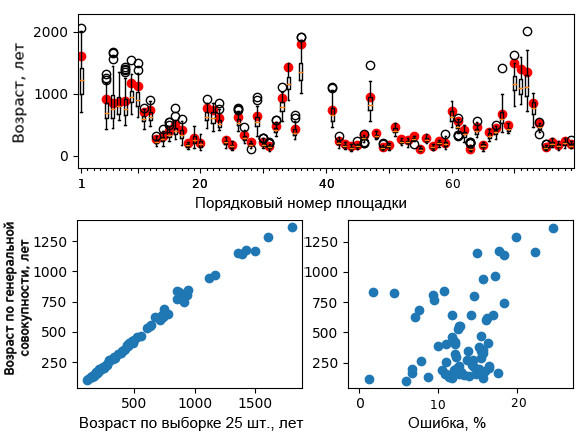
\includegraphics[width=0.8\textwidth]{authors/kolegov-fig2.jpg}
  \end{center}
  \caption{График распределения выборок (\textit{а}). Красными точками показаны истинные значения,
полученные по 100 замерам, черные боксы и кружки~--- выборки из 25 шт. Графики ошибок: \textit{б}~--- график зависимости истинных значений от выборки в 25 ед. \textit{в}~--- погрешность измерений получаемая при замере 25 шт. талломов}
  \label{fig:kolegov}
\end{figure}


\begin{changemargin}{-2cm}{-2cm}

\begin{center}
\begin{minipage}[c]{1.2\textwidth}
 \begin{table}[H]
 \begin{center}
 \caption*{\bfseries Индексы генетического разнообразия и тестов на нейтральность в исследованных популяциях}
 
 \label{tab:litvinov1}
 \medskip\small
 \begin{tabularx}{1.0\linewidth}{l c c r c r c c }
 \toprule
 %Русские юго-запад &
 \parbox[c][8em][c]{0.06\textwidth}{ \centering Про\-филь} &
 \parbox[c][8em][c]{0.10\textwidth}{ \centering Угол наклона поверхности осыпи, °} &
 \parbox[c][8em][c]{0.10\textwidth}{ \centering Длина поверхности осыпи, м} &
 \parbox[c][8em][c]{0.10\textwidth}{ \centering Площадь поверхности осыпи, м$^2$} &
 \parbox[c][8em][c]{0.08\textwidth}{ \centering Скорость транзита облом. чехла, м/год} &
 \parbox[c][8em][c]{0.12\textwidth}{ \centering Энерге\-тический потенциал, кДж} &
 \parbox[c][8em][c]{0.10\textwidth}{ \centering Удельный энергет. потенциал ($E_{\textup{уд.}}$), кДж/м$^2$} &
 \parbox[c][8em][c]{0.10\textwidth}{ \centering Удельный энергет. потенциал ($A_{\textup{уд.}}$), кДж/м$^2$}\\

 \midrule

 1 &
 30 &
 143 &
 8\,071 \hspace*{0.3cm}&
 0,67 &
 2,94$\cdot$10$^6$ &
 364,56 &
 1,70 \\
 5 &
 20 &
 194 &
 12\,620 \hspace*{0.3cm}&
 0,38 &
 4,64·10$^6$ &
 368,02 &
 0,71 \\
 8 &
 23 &
 304 &
 22\,740 \hspace*{0.3cm}&
 1,09 &
 14,62·10$^6$ &
 643,30 &
 2,30 \\
 10 &
 23 &
 108 &
 4\,014 \hspace*{0.3cm}&
 0,20 &
 0,92·10$^6$ &
 229,75 &
 0,42 \\
 11 &
 26 &
 145 &
 5\,247 \hspace*{0.3cm}&
 0,33 &
 1,77·10$^6$ &
 337,67 &
 0,76 \\
 12 &
 28 &
 118 &
 5\,000 \hspace*{0.3cm}&
 0,79 &
 1,45·10$^6$ &
 289,85 &
 1,92 \\


 \bottomrule
 \end{tabularx}
 \end{center}

 \end{table}
\end{minipage}
\end{center}
\end{changemargin}

\bigskip


\clearpage

Анализ полученных данных позволяет сделать следующие выводы:

\begin{enumerate}[noitemsep]\vspace{-8pt}
  \item Допустимо при лихенометрической съёмке производить 25 замеров талломов, при этом погрешность относительно обычной методики (100~замеров) составит 8--15\,\%;
  \item Скорость транспортировки обломков в различных частях аккумулятивной зоны варьирует от~0,17 до~0,53~м/год, при среднем значении 0,34~м/год;
  \item Динамический возраст поверхности аккумулятивной зоны варьирует от 268 до 502 лет в разных её частях;
\end{enumerate}



\begin{thebibliography}{99}
%1
\bibitem{}\BibAuthor{Галанин\,А.\,А.} Лихенометрия: современное состояние и направление развития
метода (аналитический обзор).~--- Магадан~: СВКНИИ ДВО РАН, 2002.~--- 74~с.
%2
\bibitem{}\BibAuthor{Галанин\,А.\,А.} Каменные глетчеры Северо-Востока России: строение, генезис,
возраст, географический анализ~: Дисс. $\dots$ доктора наук~: 11.00.04 / Северо-Восточный комплексный НИИ ДВО РАН.~--- Владивосток, 2009.~--- 303~с.
%3
\bibitem{}\BibAuthor{Галанин\,А.\,А., Смирнов\,В.\,Н.} Динамика гравитационных склоновых процес-
сов в горах Северного Приохотья в позднем голоцене и лихенометрическая методика их моделирования и прогноза // Геоморфология.~--- 2004.~--- №~3.~--- С.~67--75.
%4
\bibitem{}\BibAuthor{Каплина\,Т.\,И.} Криогенные склоновые процессы.~--- М.~: Наука, 1965.~--- 296~с.
%5
\bibitem{}\BibAuthor{Колегов\,П.\,П.} Динамика коллювиальных процессов в хребте Дел-Урэкчэн (Се-
верное Приохотье) на основе лихенометрических данных // Вестник СВНЦ ДВО РАН.~--- 2016.~--- №~2.~--- С.~10--18
%6
\bibitem{}\BibAuthor{Колегов\,П.\,П.} Динамика осыпей и каменных глетчеров Ольского плато (Северное Приохотье) на основании лихенометрического и фотометрического гранулометрического анализов // Вестник СВНЦ ДВО РАН.~--- 2019.~--- №~3.~--- С.~54–62.~--- DOI: 10.34078/1814-0998-2019-3-54-62.
%7
\bibitem{}\BibAuthor{Колегов\,П.\,П.} Геопространственный анализ коллювиальных конусов выноса центральной части гор Дел-Урэкчэн (Северное Приохотье) // Форум <<Наука Северо-Востока России: фундаментальные и прикладные исследования в Северной Пацифике и Арктике>>. Магадан, 5--6 марта 2020~г. / Отв. ред. Н.\,А.\,Горячев.~--- Магадан~: СВКНИИ ДВО РАН, 2020.~--- С.~41--44.
%8
\bibitem{}\BibAuthor{Суходровский\,В.\,Л.} Экзогенное рельефообразование в криолитозоне.~--- М.~:
Наука, 1979.~--- 280~с.
%9
\bibitem{}\BibAuthor{Титов\,Э.\,Э.} Скорости перемещения обломочного материала на склонах гор
Северо-Востока СССР // Вестник МГУ. География.~--- 1970.~--- №~4.~--- С.~95--98.
%10
\bibitem{}\BibAuthor{Титов\,Э.\,Э.} Строение и развитие склонов гор Северо-Востока СССР~: Автореф.
дис. $\dots$ канд. георг. наук~: 693 / Э.\,Э.\,Титов; МГУ.~--- Мoсква, 1971.~--- 35~с.

\bibitem{}ArcticDEM~--- Polar Geospatial Center.~--- 2018.~--- URL: https://www.pgc.umn.edu/data/arcticdem/ (ref. date: 20.02.2020).

\end{thebibliography}
\thispagestyle{empty}

 \procTitle{Рудные минералы Au-Ag месторождения Ирбычан: влияние фундамента на состав эпитермальной минерализации}

\procAuthor{Прийменко~В.\,В., Фомина~М.\,И., Глухов~А.\,Н., Михалицына~Т.\,И.}
\procEmail{priymenkovladimir@gmail.com, mif-74@yandex.ru, gluhov76@list.ru, tim\_66@mail.ru}
\procOrganization{СВКНИИ ДВО РАН} \procCity{Магадан}


\index{p@Прийменко~В.\,В.}
\index{g@Глухов~А.\,Н.}
\index{f@Фомина~М.\,И.}
\index{m@Михалицына~Т.\,И.}

\makeProcTitle

\textbf{Введение}

Месторождение Ирбычан расположено в~северной части Эвенского рудного района Охотско–Чукотского вулканогенного пояса (ОЧВП). Месторождение открыто в~1975~г., но слабо охарактеризовано в~литературе. В~частности, остаются неясными спектр рудных минералов и~факторы рудоконтроля.

\textbf{Геолого-структурная позиция}

Месторождение приурочено к Хивгичанской вулканической просадке, осложняющей Ирбычанскую вулкано-тектоническую депрессию (ВТД) в~зо\-не влияния Доктомычанского глубинного разлома. В~его пределах выделены три рудные зоны: Восточная, Центральная и~Северная. Рудовмещающие породы~--- игнимбриты риолитов и~дацитов, прорванные дайками андезитов, дацитов, интерсивно аргиллизированные.

\textbf{Рудная минералогия}

Определение минералов выполнено на сканирующем электронном микроскопе Jeol JSM-6510LA c энергодисперсионным спектрометром (С.-Пб., 2019. Аналитик О.~Л.~Галанкина) и на микроанализаторе Camebax (Магадан, 2020. Аналитик Е.~М.~Горячева).

Минеральный состав руд не отличается большим разнообразием. Золото-серебряная минерализация представлена электрумом, кюстелитом, акантитом, фрейбергитом, тетраэдритом, науманнитом.

В рудах установлен пирит двух генераций. Пирит~I образует ксеноморфные включения в~кварце, реже массивные агрегаты в~ассоциации с арсенопиритом; срастается с блеклой рудой, халькопиритом, сфалеритом и~акантитом; в~пиите~I наблюдаются редкие каплевидные включения пирротина. По периферии пирит~I частично или полностью замещен марказитом. Состав пирита~I стехиометричный. Пирит~II представляет собой скопления мелкокристаллических идиоморфных разностей в~кварце, формирующих, как единичные включения, так и~сфероидные формы. В~призальбандовых частях кварцевых прожилков он выполняет просечки мощностью до 1~мм. В~цементе кварцевых брекчий пирит~II приурочен к периферии обломков пород, где развивается по микротрещинам и~равномерно распределен в~них. Характерная примесь As до 1~\%. Марказит полиморфно развивается по пириту обеих генераций и~заполняет пустоты в~нем. Арсенопирит представлен идиоморфными короткопризматическими кристаллами. По соотношению As/S выделяются две его разновидности: арсенопирит~I (0,37--0,53), ассоциирующий с пиритом, и~арсенопирит~II (1,97), образующий срастания со сфалеритом. Халькопирит встречается в~виде редкой эмульсии в~сфалерите, и~в~срастании с сульфидами (пиритом, арсенопиритом, марказитом и~сфалеритом) и~блеклой рудой. Сфалерит образует срастания с пиритом~I, блеклой рудой и~халькопиритом; содержит примеси Fe (1,93--5,22~\%), Cd (0,05--0,08~\%) и~Mn (0,39~\%). Галенит встречается в~срастании с акантитом, в~нем установлена примесь Se (1,17--1,45~\%). Блеклая руда отлагается в~виде ксеноморфных обособлений, цементирующих пирит-арсенопирит-марказитовый агрегат. Срастается с халькопиритом, пиритом~I и~акантитом. По химическому составу различают фрейбергит, Fe-фрейбергит и Fe-Zn тетраэдрит. Науманнит образует тонкие минеральные смеси с акантитом. Акантит встречается в~свободном состоянии в~кварце и~в~срастании с сульфидами (пиритом, арсенопиритом, халькопиритом, сфалеритом) и~блеклыми рудами. Содержит мелкую вкрапленность электрума и~кюстелита. По данным микрозондового анализа акантит подразделяется на стехиометричный и~селенсодержащий (микропримесь Se от 0,87 до 11,51~\%). Кроме того, в~рудах установлены Ag-содержащие минеральные смеси акантита, науманнита и~блеклых руд. Электрум (самородное золото) образует срастания с акантитом и~включения в~нем. Размер его выделений от 1,5 до 7 мкм. Пробность 402--426~\permil. Кюстелит (самородное серебро) представлено небольшими округлыми включениями в~акантите размером до 15~мкм.

Выделены три минеральных парагенезиса:
\begin{enumerate}[noitemsep]\vspace{-8pt}
  \item дорудный (пирит~I~+ арсенопирит~I);
  \item рудный (блеклая руда~+ халькопирит~+ сфалерит~+ пирротин~+\\галенит~+ акантит~+ электрум~+ кюстелит);
  \item пострудный (пирит~II~+ марказит~+ арсенопирит~II).
\end{enumerate}
 \vspace{-8pt}Нашими данными не подтверждено существование золото-аргентитового парагенезиса, ранее выделенного Р.~Г.~Кравцовой [3].

 Нестехиометричность составов серебросодержащих минеральных смесей дает
 возможность предполагать одностадийность рудного процесса в резко
 градиентных условиях [6].

\textbf{Сопоставление c другими месторождениями Эвенского рудного района}

Цоколем Ирбычанской ВТД является консолидированная кора Омолонского кратонного террейна [1, 2, 4, 7]~--- в~отличие от Туромчинской ВТД, вмещающей месторождения Сопка Кварцевая, Дальнее, Невенрекан и~заложенной на образованиях Гижигинской складчатой зоны [1, 4, 5, 7]. Однако различия в обобщенных данных минерального состава руд
месторождений Сопка-Кварцевая, Дальнее, Ороч и Ирбычан [6, 8]
Технико-экономическое обоснование постоянных разведочных кондиций для
подсчета запасов золота и серебра месторождений: Сопка-Кварцевая, 2006
г, 2010 г, Ороч, 2010 г, Ирбычан, 2017 г\] указывают на то, что влияние
фундамента на него было крайне незначительным. Это также подтверждается
изотопно-геохимическими данными Р.Г. Кравцовой с соавторами \[4\].

\textit{Авторы выражают благодарность В.~В.~Акинину,  Н.~А.~Горячеву, Е.~М.~Горячевой, Е.\,Е.~Коловой, Н.~Е.~Савве (СВКНИИ ДВО РАН), С.~Ф.~Петрову, А.~П.~Бороздину (ООО~<<ЛИМС>>), О.~Л.~Галанкиной (ИГГД РАН) за содействие при выполнении данной работы.}


\begin{thebibliography}{99}

\bibitem{}
\BibAuthor{Горячев~Н.~А., Егоров~В.~Н., Савва~Н.~Е., Кузнецов~В.~М., Фомина~М.~И., Рожков~П.~Ю.} Геология и~металлогения фанерозойских комплексов юга Омолонского массива.~--- Владивосток~: Дальнаука, 2017.~--- 312~с.
\bibitem{}
\BibAuthor{Животнев~А.~Я., Литовченко~З.~И.} Структурная позиция Ирбычанского рудопроявления // Материалы по геологии и~полезным ископаемым Северо–Востока СССР.~--- 1977.~--- №~23, Кн.~1.~--- С.~162--167.
\bibitem{}
\BibAuthor{Кравцова~Р.~Г.} Геохимия и~условия формирования золото-серебряных рудообразующих систем Северного Приохотья.~--- Новосибирск~: Академическое изд-во <<Геос>>, 2010.~--- 292~с.
\bibitem{}
\BibAuthor{Кравцова~Р.~Г., Дриль~С.~И., Алмаз~Я.~А., Татарников~С.~А., Владимирова~Т.~А.} Первые данные по Rb-Sr возрасту и~изотопному составу золото-серебряных руд месторождения Дальнего (Эвенский рудный район, Северо-Восток России) // Доклады Академии Наук.~--- 2009.~--- Т.~428, №~2.~--- С.~240--243.
\bibitem{}
\BibAuthor{Костырко~Н.~А., Пляшкевич~Л.~Н., Болдырев~М.~В.} Строение и~вещественный состав рудных зон Эвенского рудного поля // Материалы по геологии и~полезным ископаемым Северо–Востока СССР.~--- 1974.~--- №~21.~--- С.~87--94.
\bibitem{}
\BibAuthor{Савва~Н.~Е.} Минералогия серебра Северо-Востока России.~--- М.~: Изд-во Триумф, 2018.~--- 544~с.
\bibitem{}
\BibAuthor{Терехов~М.~И.} Стратиграфия и~тектоника южной части Омолонского массива.~--- М.~: Наука, 1979.~--- 114~с.
\bibitem{}Технико-экономическое обоснование постоянных разведочных кондиций для подсчета запасов золота и серебра месторождений: Сопка-Кварцевая, 2006\,г, 2010\,г, Ороч, 2010\,г, Ирбычан, 2017\,г.~--- Магадан\,:АО <<Полиметалл>>, 2006.

\end{thebibliography}


\rasdel{Анализ и состояние объектов окружающей среды}
\procTitle{Разработка оптимальной методики БПЛА-фотограмметрии для обеспечения обследования и~мониторинга оползневых процессов и~мест возможного обрушения крутых склонов Кругобайкальской железной дороги}

\procAuthor{Ерофеев~В.\,В., Яхин~А.\,М., Савин~А.\,С., Паршин~А.\,В.}
\procEmail{erofeev.vladimir1997@mail.ru}
\procOrganization{ИРНИТУ, Siberian School of Geosciences} \procCity{Иркутск}


\index{e@Ерофеев~В.\,В.}
\index{p@Паршин~А.\,В.}
\index{s@Савин~А.\,С.}
\index{z@Яхин~А.\,М.}

\makeProcTitleRazdel


\textbf{Введение}

Моделирование местности и~мониторинг ее изменений с~помощью беспилотных систем является одной из лучших практик последнего времени, существенно снизивших нагрузку на~специалистов, выполняющих обследования природных и~техногенных объектов, расположенных на~участках со~сложной морфологией рельефа [5]. При этом успешно применяются методы лидарного сканирования [4] и~аэрофотосъемки с~последующей фотограмметрической обработкой. Теория и~практика таких съёмок уже достаточно хорошо разработана, и~они широко применяются для решения инженерных, геологических, горных и~других задач [1, 2, 6], однако периодически встречаются специфические объекты [3--5], на~которых классические варианты методик могут быть неэффективными.

Одним из таких объектов является Кругобайкальская железная дорога (Иркутская область, Россия), которая представляет собой уникальный природно-антропогенный комплекс. Железнодорожные пути находятся на~уступе, созданном в~результате взрывов, в~следствии этого с~одной стороны непосредственно от полотна находится воды озера Байкал, а с~другой отвесные скалы, достигающие угла наклона вплоть до 80 градусов, в~результате чего на~данном участке часто происходят обвалы, повреждающие не только ЖД пути, но и~электрокоммуникации, а также укрепления земного полотна от размыва и~волноприбоя, что приводит к ускорению разрушения уступа. Экономические и~трудовые затраты на~ремонт повреждённых участков являются существенными, а отслеживание мест возможного обрушения пешеходным методом является опасным и~времязатратным и~не обеспечивает полной картины состояния откоса. Поэтому задача создания комплекса и~методов выполнения аэрофотограмметрии для мониторинга оползневых процессов и~мест возможного обрушения крутых склонов Кругобайкальской железной дороги (КБЖД) является весьма актуальной.
\clearpage
При выполнении данного кейса были обнаружены следующие проблемы, которые было необходимо решить:
\begin{enumerate}[noitemsep]\vspace{-8pt}
\item Применение классической методики аэрофотограмметрии (съёмка в~надир) не представляется возможным в~виду больших углов наклона горного массива достигающих 80 градусов, при такой съёмке возникает ряд проблем, таких как сложность фокусировки камеры, в~пределах одного кадра перепад высот составляет сотни метров, существенно различный размер пикселя в~разных частях фото, и~ряд других, что~приводит к некорректному результату (рис.~1).

\begin{figure}[h!]
  \begin{center}
    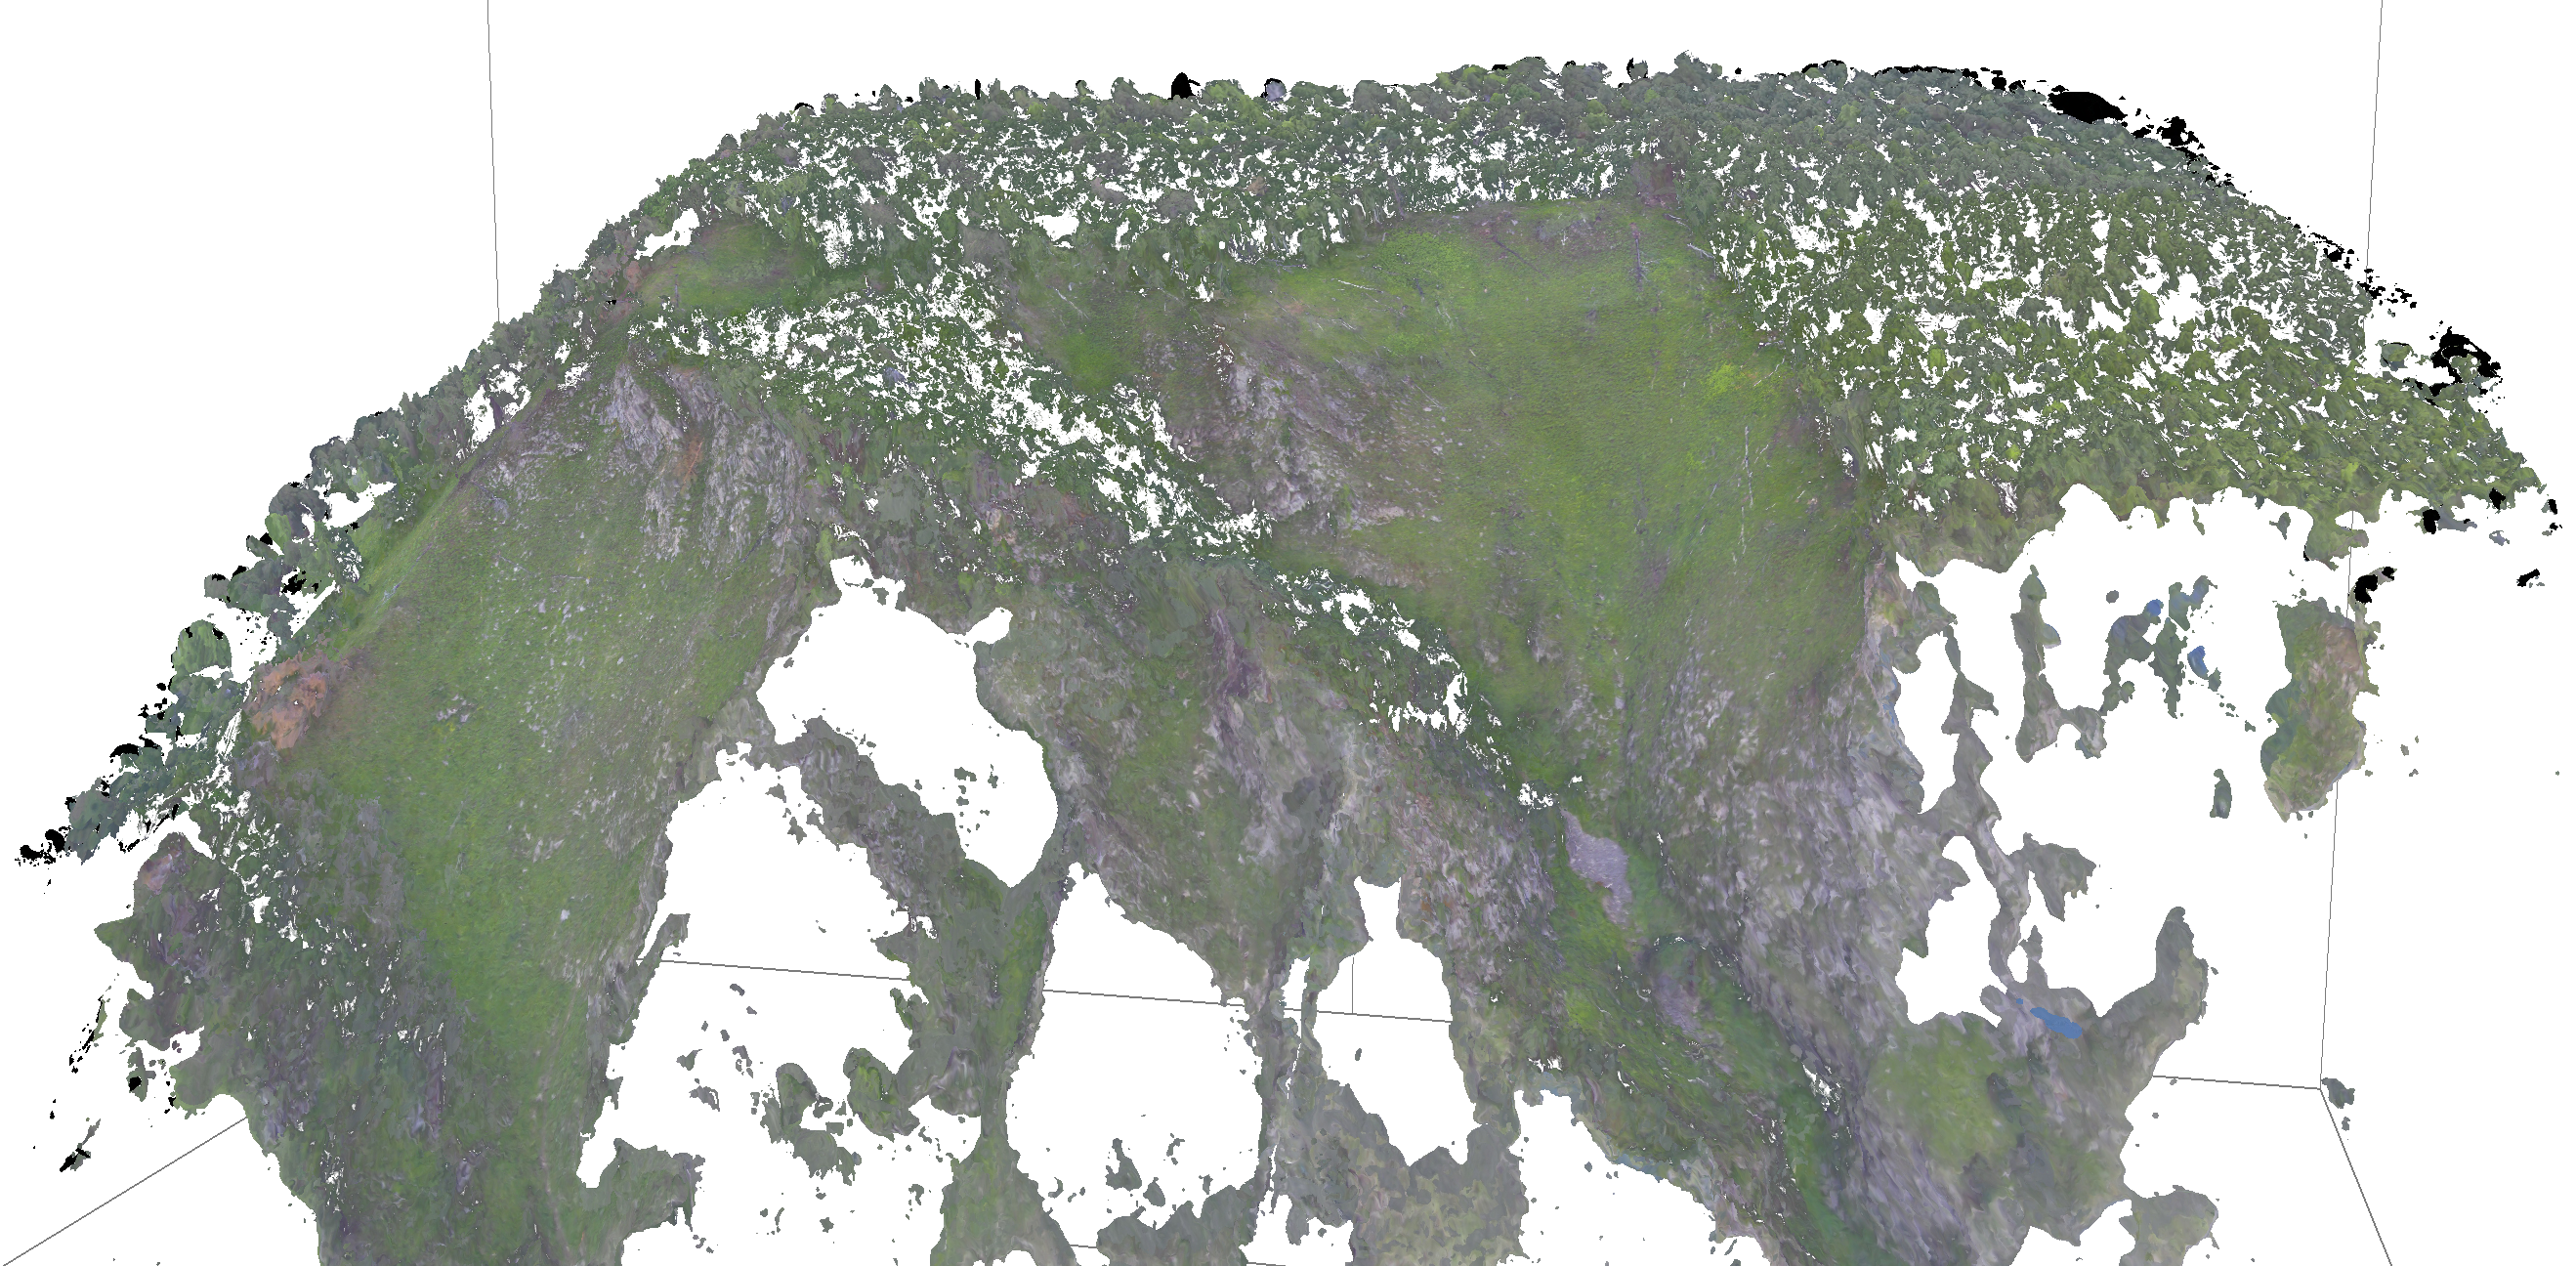
\includegraphics[width=0.9\textwidth]{authors/efremov-fig1.png}
  \end{center}
  \caption{Тайловая модель при выполнении съёмки с углом наклона камеры 90\dg}
  \label{fig:efremov-fig1}
\end{figure}


\item Съёмка по~методике, аналогичной моделированию зданий, включающая комбинирование наземных и~аэрофотограмметрических работ с~различными углами наклона камер слишком трудоёмка для мониторинга большого количества объектов площадью как~минимум по~нескольку квадратных километров.
\item Необходимо подбирать оптимальные по~соотношению <<качество результата/экономика работ>> модели фотокамер, в~том числе и~оборудования с~режимом съёмки в~мультиспектральном спектре, с~учётом желательной минимизации массы и~стоимости владения комплексом, высокой точности и~детальности реконструкции местности, возможности работы при отрицательных температурах, достижения времени полёта не менее 1~часа.
\item Выбор наиболее подходящего программного обеспечения для обработки и~анализа материалов съёмки, как проприетарного, так и~бесплатного, для сравнительной характеристики и~предоставления результата специалистам ООО <<РЖД>>.
\item Создание компактного комплекса для возможности выполнения работы партией из~двух человек и~минимальным временем на~развёртку.

\end{enumerate}
\vspace{-8pt}

\textbf{Применяемое оборудование}

При выполнении поставленной задачи было использовано следующее оборудование:

\begin{itemize}[noitemsep]\vspace{-8pt}
\item тяжёлый гексакоптер SibGIS UAS (Unmanned Aerial System) (рис.~2);
\item двухосевые и~трехосевые гиростабилизированные подвесы лёгкого и~среднего классов.
\end{itemize}
\vspace{-8pt}

\begin{figure}[h!]
  \begin{center}
    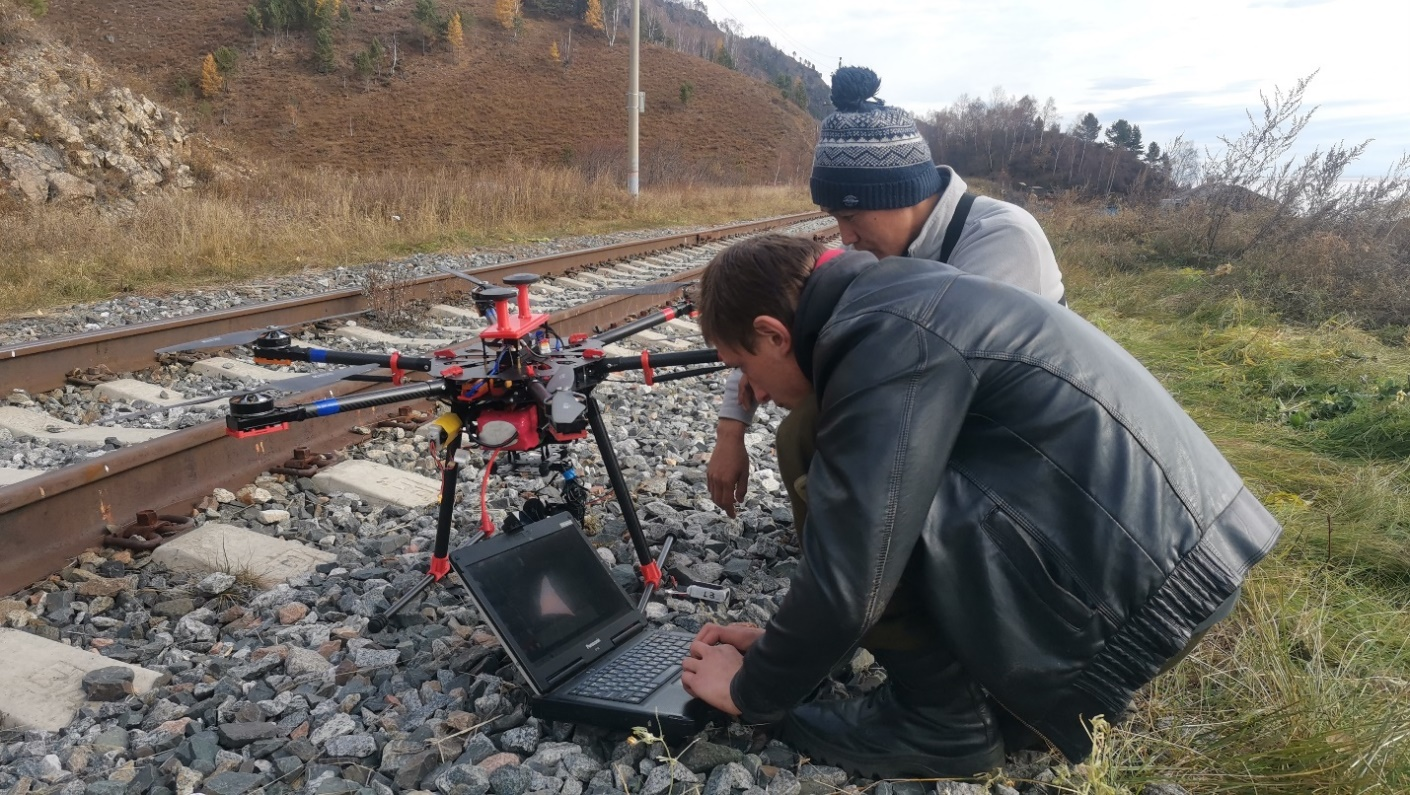
\includegraphics[width=0.9\textwidth]{authors/efremov-fig2.jpg}
  \end{center}
  \caption{Настройка комплекса на КБЖД}
  \label{fig:efremov-fig2}
\end{figure}


Камеры:

\begin{itemize}[noitemsep]\vspace{-8pt}
\item специализированные лёгкие камеры для аэрофотосъёмки Mapir Survey 2 и~3;
\item неспециализированные, но подходящие для аэрофотосъёмки модели лёгких защищённых экшен-камер и~компактных цифровых фотокамер, такие как Sony RX0 и~GitUp Git3D;
\item B2B-фотокамеры семейства Sony QX/UMC.
\end{itemize}
\vspace{-8pt}

\textbf{Методика выполнения работ}

Для сбора необходимых нам данных было выполнено три серии опытно-методических съёмок на~опытном участке КБЖД, характеризующимся сложным рельефа, сопоставимым с~рельефом на~всей протяжённости железной дороги. Во всех трёх сериях использовался тяжёлый гексакоптер SibGIS UAS, который может переносить самые тяжёлые камеры и~подвесы, в~дальнейшем съёмку планируется проводить с~помощью более лёгкого БПЛА. Первые съёмки производились по~отработанной методике создания ЦМР, которую наш коллектив применяет в~геологической практике, а последующие работы были направлены на~оптимизацию технологии для данных условий.

После прибытия команды на~точку, откуда совершались полёты, производится развёртка оборудования: гексакоптер приводится в~рабочее положение, устанавливается базовая станция дифференциальной геодезической системы, применение которой необходимо для~создания точно привязанных центров фотографирования. Поскольку съёмка велась в~безреперном варианте, то <<базе>> дифференциальной станции требуется время на~позиционирование, для усреднения и~точной фиксации своего местоположения, после чего она будет передавать поправки на~ровер (в нашем случае в~качестве ровера выступает компьютер-компаньон полётного контроллера гексакоптера и~используются его GNSS-антенны), в~реальном времени. Выбор между внесением поправок при постобработке и~съёмки в~режиме кинематики реального времени~--- RTK сделан в~пользу последней, поскольку в~рамках данного класса задач размеры исследуемых участков не превышают первых десятков квадратных километров и~радиосвязь между базой и~ровером не теряется, а обработка требует меньших временных затрат.

Подвесы с~закреплёнными на~них камерами приводятся в~положение под необходимым углом.
\clearpage
С помощью специального модуля SibGIS Flight Planner (Паршин и~Морозов, 2017) [7] формируются полётные миссии, представляющие собой массив точек <<долгота~-- широта~-- высота>>, находящихся на~постоянной высоте над рельефом. Необходимая для этого цифровая модель рельефа создана заранее на~основе спутниковых данных Intermap Nextmap. Участок работ характеризуется перепадом высот в~несколько сотен метров, выполнять в~таких условиях фотосъёмку с~одного уровня, или даже с~грубым обтеканием рельефа недопустимо, это приведёт к сложностям и~потере качества при обработке. Съёмка выполняется по~сети параллельных маршрутов, в~обычном случае скорость, высота и~продольное перекрытие между кадрами съёмки составляет 70--80\,\%, поперченное~--- 60--70\,\%. Съёмка велась на~высоте 125~м ($\sim$3--5~см/пиксель в~зависимости от применяемой камеры).

После проведения полевых работ выполняется обработка полученных данных съёмки. Если камера или её компьютер-компаньон не оснащены собственным GNSS-приёмником, перед каждым полётом производится синхронизация часов камеры с~точным временем.

На заключительном этапе выполняется фотограмметрическая обработка данных съёмки для получения 3D-моделей и~ортофотоплана.

Первая серия ОМР производилась со~съёмкой в~надир, затем были апробированы различные углы камеры: 45, 60 и~90 градусов, с~обработкой вместе и~по отдельности, в~различных комбинациях (рис.~3).

\begin{figure}[h!]
  \begin{center}
    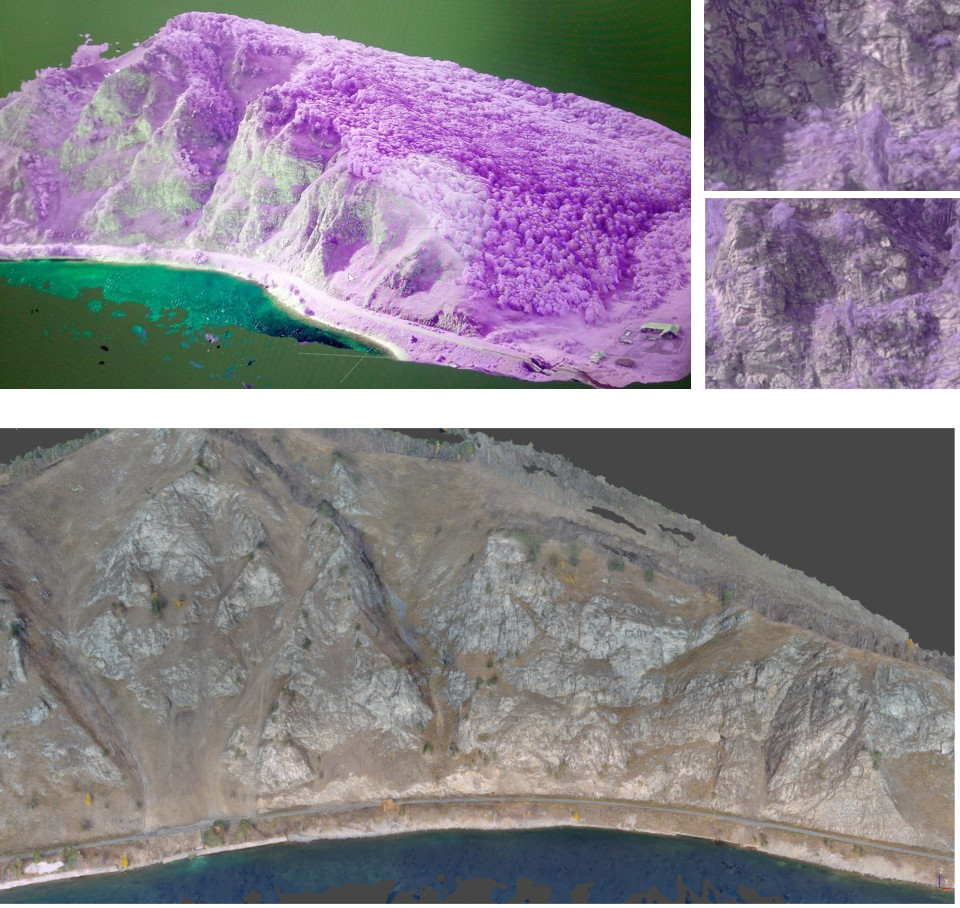
\includegraphics[width=0.9\textwidth]{authors/efremov-fig3.jpg}
  \end{center}
  \caption{Тайловая модель, построенная по результатам съёмки с углами наклона камеры 45 и 90 градусов: сверху~--- инфракрасный канал и крупные фрагменты модели; снизу~--- видимый диапазон)}
  \label{fig:efremov-fig3}
\end{figure}

\clearpage
\textbf{Выводы}

В результате проведённых исследований сделаны следующие заключения:
\begin{enumerate}[noitemsep]\vspace{-8pt}
\item Для получения полного объёма данных для построения детальной 3D модели достаточно производить съёмку с~двух углов наклона камеры, 45 и~90 (в надир) градусов.
\item При обработке фотографий следует заменять координаты в~метаданных фотоснимков с~камеры (если на~таковой установлен GPS модуль) на~координаты, взятые с~контроллера полётов, на~основе единства точного времени, записанного камерой и~ровером, поскольку для определения координат ровера используется дифференциальная станция, с~более точным определением местоположения.
\item Применение мультиспектральной камеры весьма желательно поскольку позволяет более контрастно выделять трещины и~разломы на~тайловой модели. В перспективе это~создаст предпосылки для автоматизации дешифрирования опасных обстановок.
\item Использование трёхосевого подвеса, в~отличие от двухосевого, позволяет фиксировать камеру во всех трёх положениях, что даёт большую устойчивость, а при съёмке с~наклоном камеры не приходится менять настройки полёта, что бы гексакоптер не~разворачивался при переходе на~соседний профиль.
\item Мониторинг склонов КБЖД с~использованием аэрофотограмметрии даёт более полное представление о состоянии массива, чем пеший обзор местности.
\item Применяемый метод и~оборудование возможно использовать не только на~участках КБЖД, но и~на других участках со~схожей проблематикой и~рельефом.
\end{enumerate}
\vspace{-8pt}

\begin{thebibliography}{99}

\bibitem{}\BibAuthor{Паршин А.~В., Морозов В.~А.} Навигационный модуль <<SibGIS Flight Planner>> // Свидетельство о регистрации программы для ЭВМ RU~2017615422, 16.05.2017.~--- Заявка №~2017612307 от 21.03.2017.
\bibitem{}\BibAuthor{Ahokas~J., Le Guern~P. Slettemeas~T., Syrdalen~E., et al.} Case-Study of Using Unmanned Aerial Vehicles for a Better Characterization of the Barents Sea Subsurface // First EAGE Workshop on Unmanned Aerial Vehicles.~--- Toulouse, 2019.~--- DOI:~10.3997/2214-4609.201903328.
\bibitem{}\BibAuthor{Bubniak I. M., Bubniak A. M., Gavrilenko O. D., Nikulishyn V. I., Golubinka I. I.}. Using laser scanning and digital photogrammetry for creation of virtual geological outcrops: case studies from the west of Ukraine // 18th International Conference on Geoinformatics~--- Theoretical and Applied Aspects. May 13--16, 2019. Kiev, Ukraine.~--- Kiev, 2019.~---DOI: 10.3997/2214-4609.201902078.
\bibitem{}Geological models using digital outcrops from photogrammetry.~--- URL: https://www.georeka.com/geological\--models\--using\--digital\--outcrops\--from\--photogrammetry (ref. date: 26.10.2020).
\bibitem{}\BibAuthor{Parshin A.~V., Budyak A.~E., Babyak V.~N.}. Interpretation of Integrated Aerial Geophysical Surveys by Unmanned Aerial Vehicles in Mining: a Case of Additional Flank Exploration // IOP Conf. Ser.: Earth Environ. Sci. 459 052079.~--- 2020.~--- DOI:~10.1088/1755-1315/459/5/052079.
\bibitem{}\BibAuthor{Parshin~A., Budyak~A., Chebokchinov~I., Sapunov~V., Bulnayev~A., Morozov~V.} Complex UAS-Geophysical Surveys at the First Stages of Geological Prospecting: Case in the Western Sayan (Russia) // First EAGE Workshop on Unmanned Aerial Vehicles.~--- Toulouse, 2019.~--- DOI:~10.3997/2214-4609.201903321.
\bibitem{}\BibAuthor{Rocca R}. Enhancing and Sharing Drone 3D Models with Geological Interpretation Using Move, Blender and Sketchfab Software // First EAGE Workshop on Unmanned Aerial Vehicles, Dec 2019.~--- Toulouse, 2019.~--- DOI: 10.3997/2214-4609.201903331.
\end{thebibliography}

\procTitle{Перспективные методы биологической рекультивации на отвалах Якутии}

\procAuthor{Никифоров~А.\,А., Миронова~С.\,И., Гаврильева~Л.\,Д.}
\procEmail{aloooosha1991@mail.ru, mironova47@mail.ru, adoxa@mail.ru}
\procOrganization{НИИПЭС СВФУ} \procCity{Якутск}


\index{n@Никифоров~А.\,А.}
\index{m@Миронова~С.\,И.}
\index{g@Гаврильева~Л.\,Д.}

\makeProcTitle

Нарушение земель происходит при разработке месторождений полезных ископаемых, прокладке трубопроводов, проведении строительных, мелиоративных, лесозаготовительных, геологоразведочных, испытательных, эксплуатационных, проектно-изыскательных и иных работ, поэтому на Севере нашей страны актуальны вопросы их восстановления с применением наиболее эффективных и экономически целесообразными способами. Практическое применение на территории Республики Саха (Якутия) на нарушенных землях предприятий, занимающих алмазодобычей, угля и на россыпных месторождениях золота находятся только на опытно-экспериментальных стадиях и имеют только рекомендательный характер.  Применение старики (ветоши) для биологической рекультивации на отвалах пустых пород карьера <<Айхал>> проведена впервые на нарушенных территориях крайнего Севера. Старика (ветошь)~--- сухая прошлогодняя трава на лугах, опавшие листья. В её состав входят все не скошенные растения или отава после сенокошения, т.\,е. это луговые злаки, бобовые и разнотравье, а также реже осоковые растения.

\textbf{Целью} работы является поиск наиболее эффективных способов для восстановления нарушенных земель добывающих предприятий.

\textbf{В задачи} работы входила оценка основных факторов, воздействующих на зарастание отвалов растительностью, проведение опытно-экс\-пе\-ри\-мен\-таль\-ных работ с применением нетрадиционного материала, оценка эффективности способа, рассмотреть возможность внедрения способа в промышленных масштабах.

\textbf{Материалы и методы исследования}

Первые опытные работы по биологической рекультивации на отвалах алмазодобывающей промышленности в республике были проведены сотрудниками Института «Якутнипроалмаз» на участке площадью 2\,га, отсыпанном плодородным слоем разной мощности, испытаны 19 видов многолетних трав [1].

С развитием промышленных предприятий резко увеличилось территории нарушенных земель, который в первую очередь разрушается почвенно-растительный покров, который приводит цепочку действий, подвергающих различные изменения территории. На нарушенных территориях образуются хвостохранилища, отвалы пустых пород, карьеры и другие [2].

Начиная с 2010\,г. институтом прикладной экологии Севера СВФУ, проведены опытно-экспериментальные работы на отвалах пустых пород карьера <<Айхал>> и в 2018\,г. на отвалах угольного разреза <<Кангаласский>> с применением нетрадиционных материалов. При рекогносцировочном исследовании поверхности отвала выбрали наиболее ровную поверхность и откосы с наименьшим углом (45\dg), высота отвала 60--70 м (рис. 1).

При заложении площадки очистили от крупных валунов и глыб, размер площадки 20$\times$20\,м, на откосе 10$\times$10\,м. Вначале на опытно-экс\-пе\-ри\-мен\-таль\-ной площадке проведён посев семян из расчёта 30\,кг/га и внесение минеральных удобрений (<<Азофоска>>) из расчета 100\,кг/га действующего вещества. Сверху площадка была накрыта старикой (ветошью), закрепили тонким слоем песка и камнями (рис. 2).

Геоботаническое описание опытно-экспериментальной площадки проводилось с учетом общего проективного покрытия в процентах, средней высоты, видового состава, проективного покрытия с применением шкалы Б.\,М.\,Миркина [3].

Сбор старики (ветоши) проводился по долине р.\,Сохсолох с помощью косилок, вил и другими ручными инструментами. Для угольного разреза <<Кангаласский>> был применён прошлогодний рулон сена, который вполне подходит для проведения опытно-экспериментальных работ.

\textbf{Результаты исследований и их обсуждение}

На опытно-экспериментальной площадке в отвале пустых пород карьера <<Айхал>> среднее проективное покрытие травостоя в первый год составило 40\,\%, на второй год 50\,\%, а максимального значения достигла 80\,\%, средняя высота травостоя в первый год 3\,см, а на второй год достигла 45\,см. Видовой состав в первом году (2011\,г.) составлял в количестве от 1--2, на последующие годы увеличилось до 7\,видов (рис. 3).

\begin{figure}
  \begin{center}
    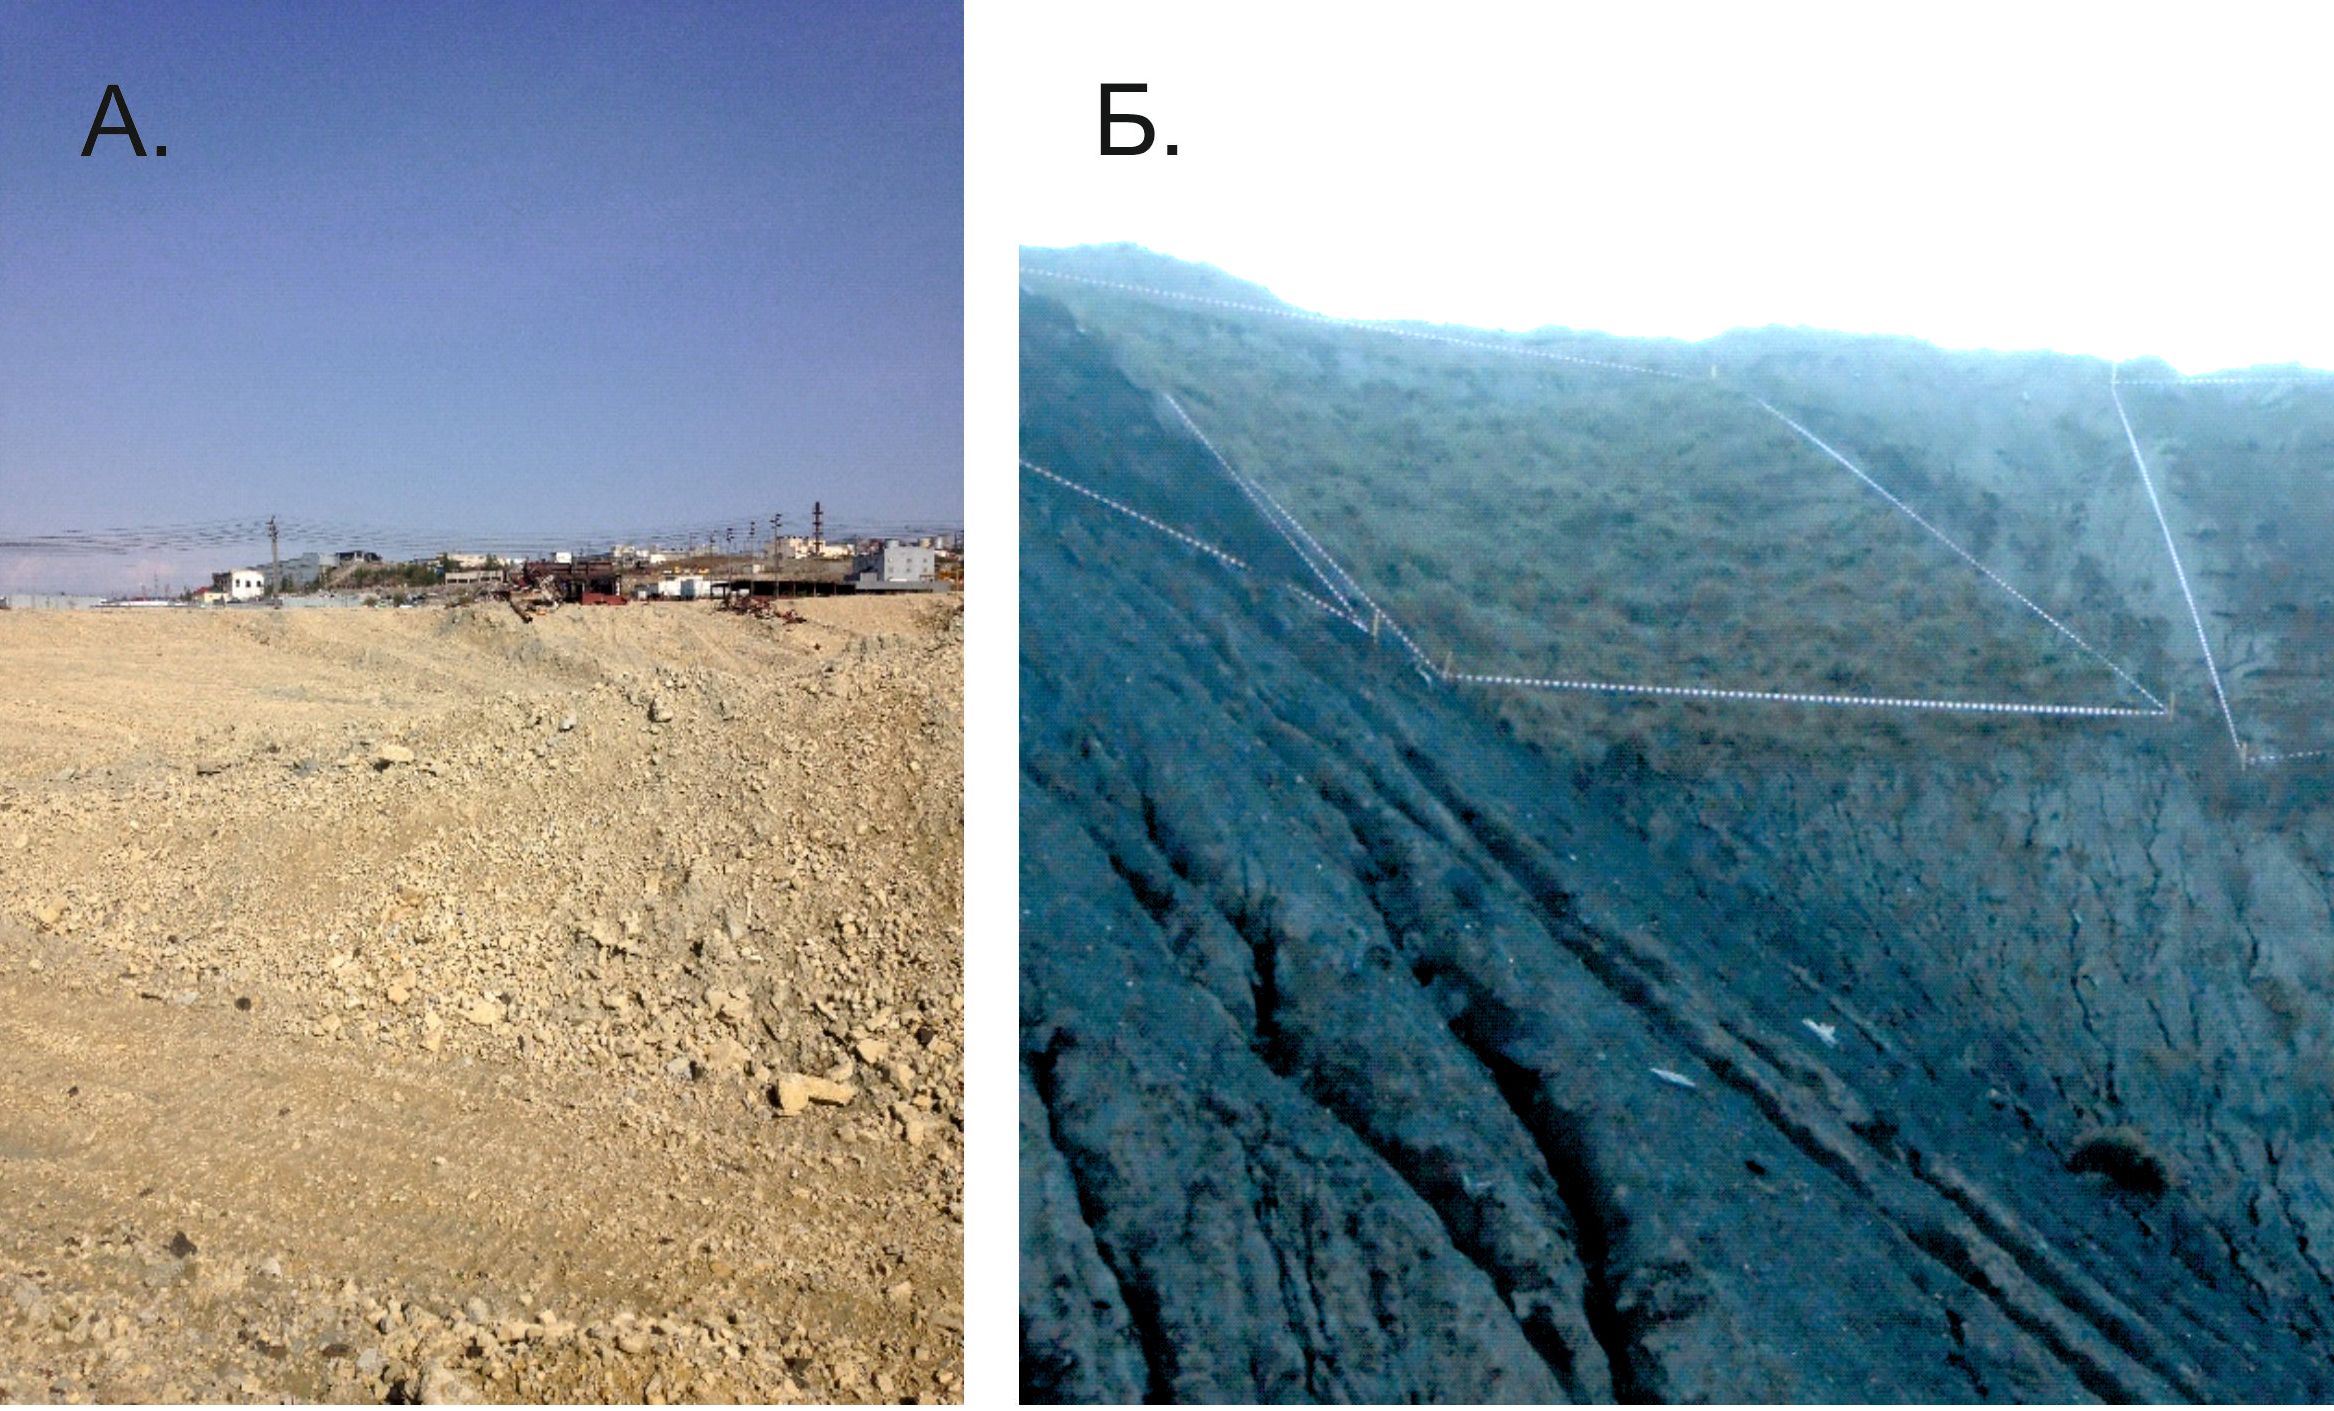
\includegraphics[width=0.9\textwidth]{authors/nekiforov-fig1.jpg}
  \end{center}
  \caption{Поверхность отвала пустых пород карьера <<Айхал>> (А) и откос отвала угольного разреза <<Кангаласский>> (Б)}
  \label{fig:nekiforov-fig1}
\end{figure}

\begin{figure}
  \begin{center}
    
\includegraphics[width=0.9\textwidth]{authors/nekiforov-fig2.jpg}
  \end{center}
  \caption{Опытно-экспериментальная площадка, накрытая старикой:
  А~--- отвал пустых пород карьера <<Айхал>>; Б~-- отвал угольного разреза <<Кангаласский>>}
  \label{fig:nekiforov-fig2}
\end{figure}

\begin{figure}
  \begin{center}
    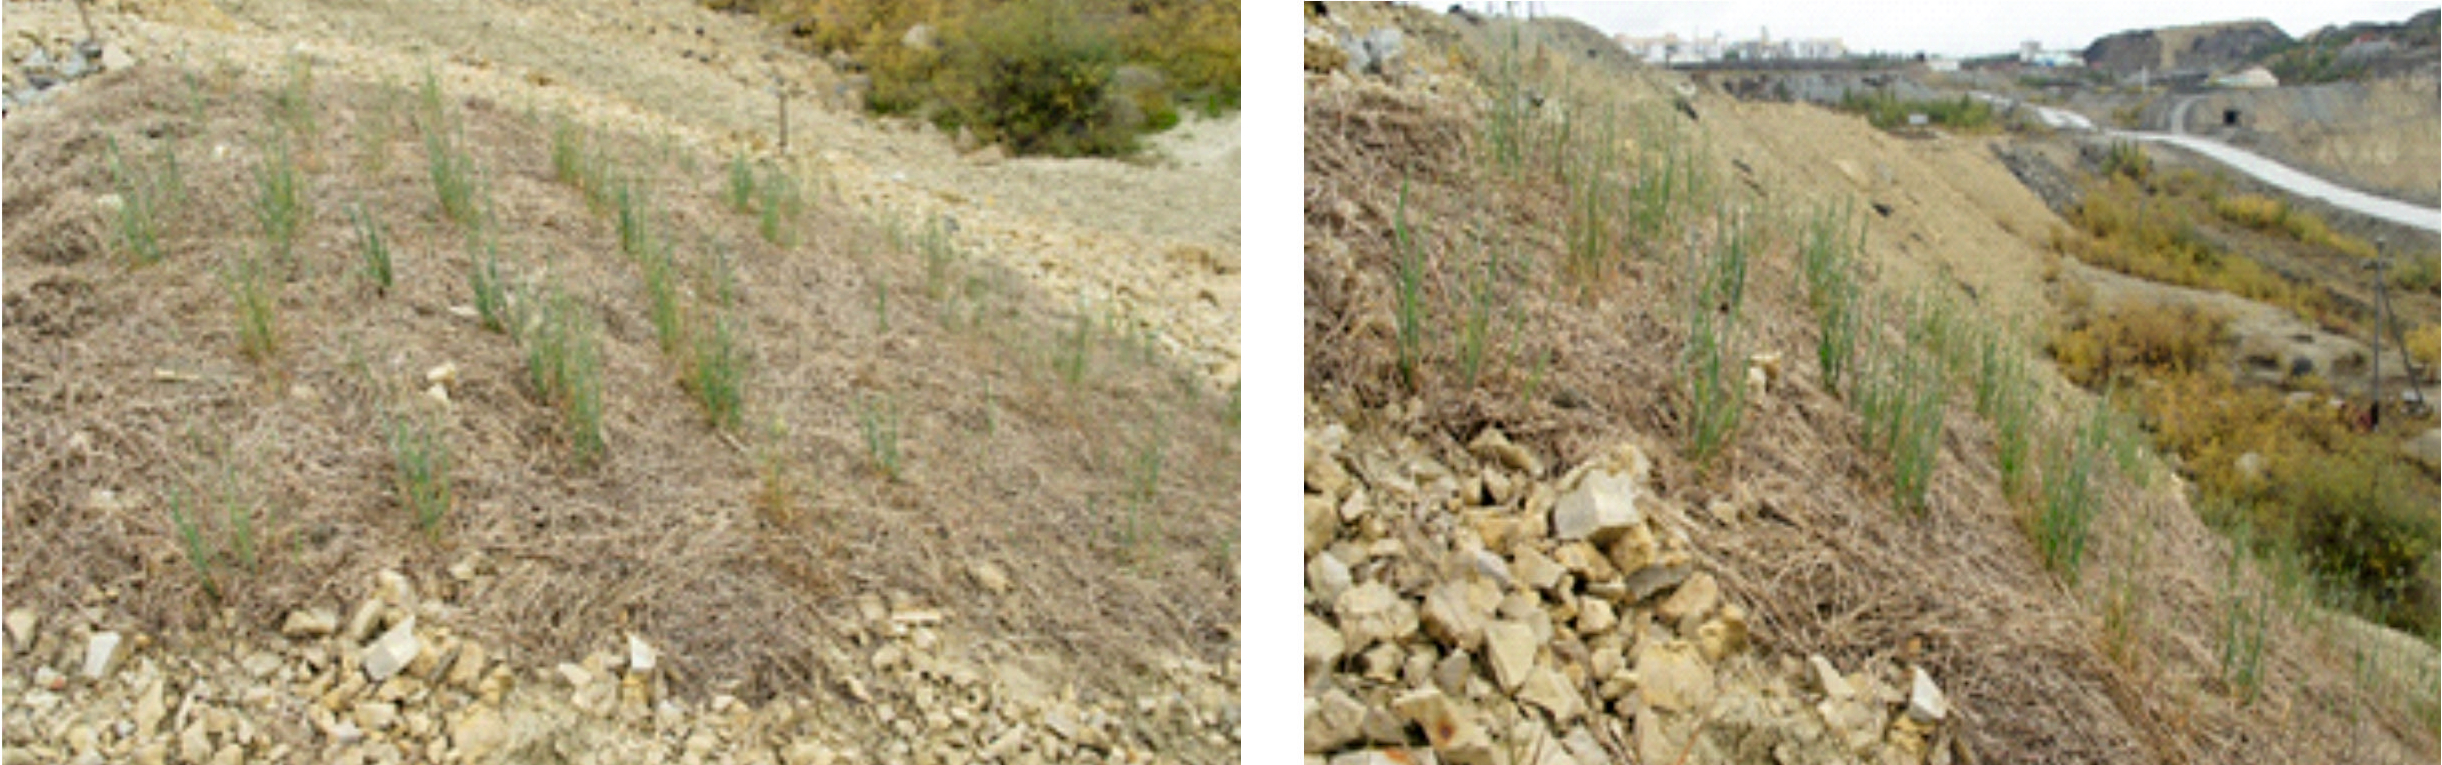
\includegraphics[width=0.9\textwidth]{authors/nekiforov-fig3.jpg}
  \end{center}
  \caption{Опытно-экспериментальная площадка с применением старики (ветоши) на отвале пустых пород карьера <<Айхал>>}
  \label{fig:nekiforov-fig3}
\end{figure}


На опытно-экспериментальной площадке в отвале угольного разреза <<Кангаласский>> среднее проективное покрытие травостоя на май месяц наблюдений составило 40--50\,\%, средняя высота 10--15\,см (май), видны всходы злаков и разнотравья. При наблюдении в июне месяце общее проективное покрытие составило 50-60\,\%, всхожесть высеянных трав составило 80\,\%, видовой состав насчитывалось до 7 видов (рис. 4).

\begin{figure}
  \begin{center}
    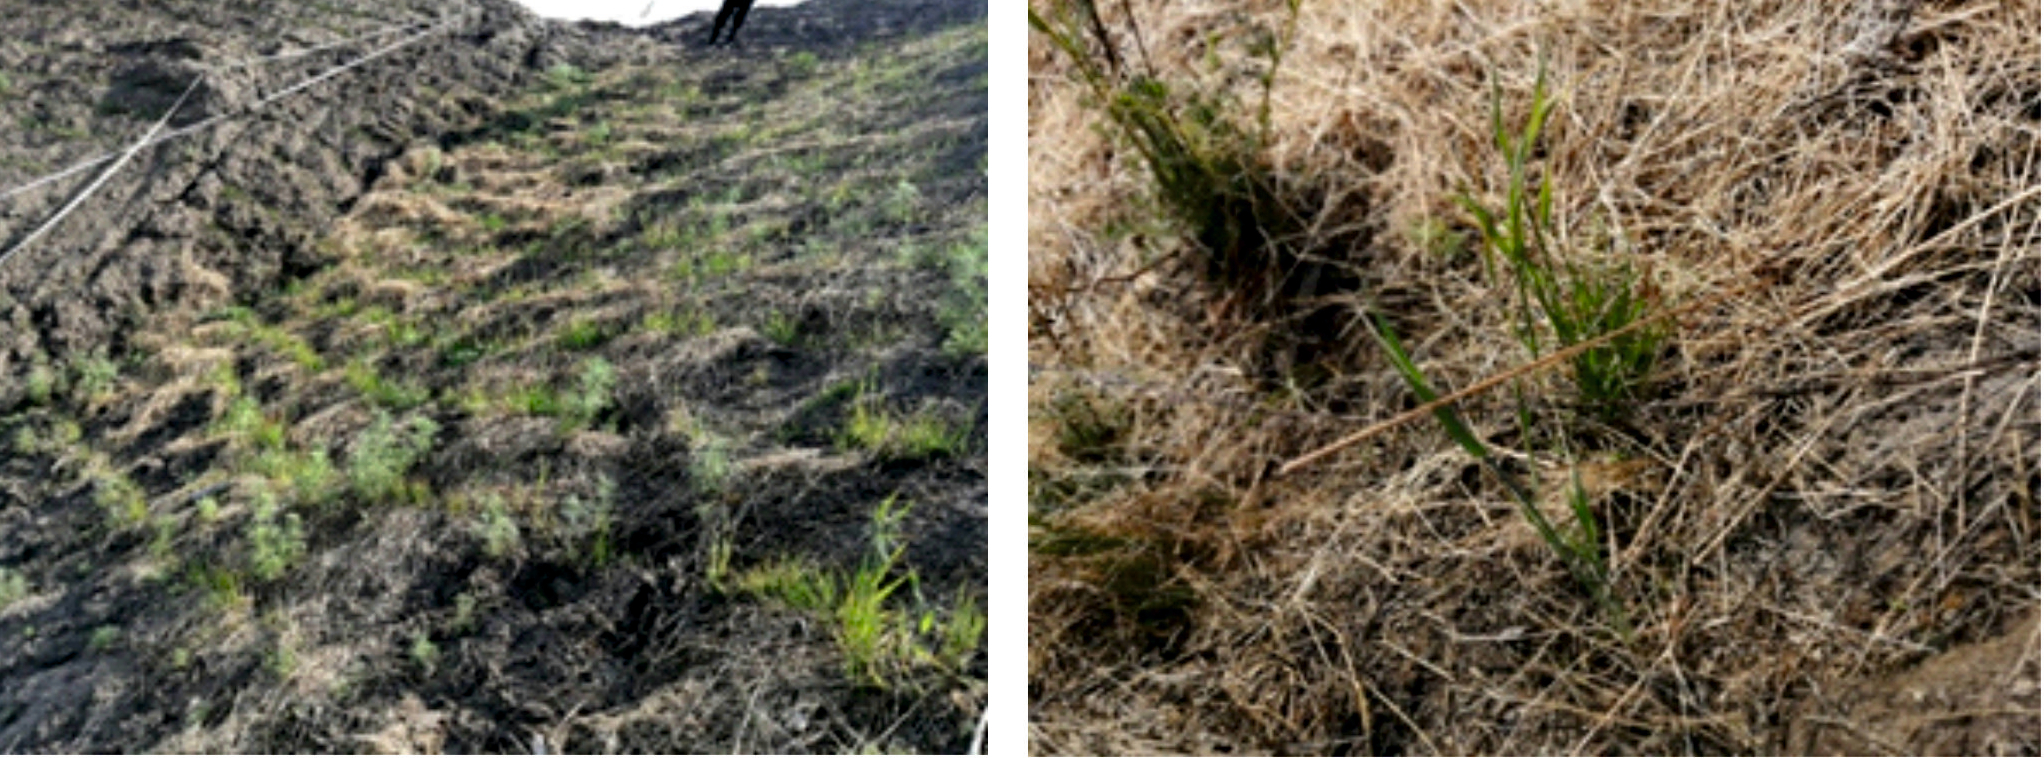
\includegraphics[width=0.9\textwidth]{authors/nekiforov-fig4.jpg}
  \end{center}
  \caption{Опытно-экспериментальная площадка с применением старики (ветоши) на отвале угольного разреза <<Кангаласский>>}
  \label{fig:nekiforov-fig4}
\end{figure}


Способ показал с перспективной стороны для внедрения в промышленных масштабах с учётом разработки технологий сбора и применения на более больших территориях. Применения старики в биологической рекультивации отвалов алмазодобычи в республике проведены впервые. В других странах этот метод применяют для других целей и в небольших объёмах только для огородов, теплицах, чаще всего в частном секторе. К применению нетрадиционного способа подтолкнуло именно условие нашего региона~--- это суровые климатические условия, экономическая целесообразность, отсутствие на данной территории потенциально плодородного слоя для отсыпки отвалов.
\clearpage
В других регионах России и мира отсыпка потенциально плодородным слоем нарушенных земель при биологической рекультивации обязательна. В нашей ситуации отсыпка плодородного слоя фактически невозможна в связи с их отсутствием, или экономической нецелесообразности их отсыпки, учитывая характер подстилающих пород траппового характера.

\textbf{Выводы}

В результате опытно-экспериментальных работ по биологической рекультивации отвалов карьера <<Айхал>> и отвалов угольного разреза <<Кангаласский>> способ применения старики (ветоши) показал наиболее эффективные результаты.

В последующем мало затратный способ можно, осуществлять повсеместно как укрывной материал без привязки к сезонным изменениям, а также в условиях отсутствия регулярного полива старика (ветошь) может, послужит задерживанием влаги и защитным слоем для всхожести семян, а при разложении питательным субстратом для роста и питания растений.

\begin{thebibliography}{99}

\bibitem{}
\BibAuthor{Лебедева\,H.\,A., Лонкунова\,А.\,Я.} Биологическая рекультивация земель, нарушенных при добыче алмазов в Якутии // Растения и промышленная среда.~--- Свердловск, 1990.~--- 71--75\,с.

\bibitem{}
ГОСТ Р 57446-2017. Наилучшие доступные технологии. Рекультивация нарушенных земель и земельных участков. Восстановление биологического разнообразия (с Поправкой).~--- Москва: Стандартинформ, 2019.~--- 47\,с.

\bibitem{}
\BibAuthor{Миркин\,Б.\,М.} Методика указания для практикума по классификации растительности методом Браун-Бланке.~--- Уфа, 1985.~--- 32\,с.
\end{thebibliography}




 \rasdel{ Медицинские и экологические проблемы северных территорий}
\vspace{-16pt}
\procTitle{Результаты кариотип диагностики плаценты и~хориона}

\procAuthorI{Абдурашидова~М.\,Б., Пак~И.\,В.}
\procEmailI{muniraxon.91@mail.ru, pakiv57@mail.ru}
\procOrganizationI{ФГАОУ ВО ТюмГУ}
\procCityI{Тюмень}

\procAuthorII{Винокурова~Е.\,А.}
\procEmailII{vinokurovaelena@mail.ru}
\procOrganizationII{ФГБОУ ВО Тюменский~ГМУ Минздрава~России}
\procCityII{Тюмень}

\makeProcTitleIIRazdel
\index{a@Абдурашидова~М.\,Б}
\index{p@Пак~И.\,В.}
\index{v@Винокурова~Е.\,А.}

\textbf{Введение}. Пренатальная диагностика за последние десятилетия добилась больших успехов в~профилактике наследственных заболеваний и~пороков развития у~плода, что способствовало уменьшению количества мертворождённых детей и~рождений детей с патологиями развития [5,9]. Развитие и~внедрение новых инновационных методов в~пренатальную инвазивную диагностику (ИПД) является одним из важных изменений в~структуре и~в~методике исследования. С помощью инвазивных методов исследования, в~основе которых лежит кариотипирование, можно прогнозировать проявление патологий со 100\,\%-ной точностью [1,7]. При этом снижение летального риска для плода является одним из основных задач в~ИПД [3]. Пренатальная диагностика (ПД) даёт возможность определить хромосомные аномалии и~пороки развития в~ранние сроки беременности, что позволяет сделать выбор беременным женщинам: прервать беременность или пролонгировать беременность [4,10-11]. При пренатальной диагностике неоценима роль кариотипирования. Кариотипирование является цитогенетическим методом диагностики хромосомных аномалий, позволяющим определить отклонения в~числе, а также в~структуре хромосом [2,5]. Нарушения в~кариотипе могут привести к наследственной патологии и~рождению детей с аномалиями развития, а также могут быть причиной бесплодия или возникновения абортусов [6,8]. Кариотипирование исследует количество хромосом, их форму, размеры, а также особенности строения хромосом. Проблема кариотип диагностики всегда была актуальной проблемой не только в~области здравоохранения, затрагивая аспекты генетики.

\textbf{Цель работы}. Изучить применение метода кариотипирования с помощью методов ИПД биопсии плаценты и~хориона у~беременных женщин в~возрасте от~16 до~46~лет.

\textbf{Материалы и~методы исследования}. Исследования были проведены на базе Государственного бюджетного учреждения здравоохранения Тюменской области <<Перинатальный центр>> г.~Тюмени. Объектом исследования являлся биоптат на основе абортного материала, который поступил в~цитогенетическую лабораторию Перинатального центра в~2019--2020~гг. Приготовление препаратов из биологического материала, взятого с помощью биопсии хориона и~плаценты пациента, включает в~себя несколько этапов: получение материала из ворсин хориона и~плаценты; фиксация препаратов; приготовление препарата; окрашивание препарата. Просматривали препарат под микроскопом, фиксируя хромосомные нарушения. Исходя из цели нашего исследования, нами было отобраны результаты изучения данных кариотипирования 544~плодов. Биологические материалы для исследования были получены путём биопсии хориона и~плацентоцентеза, от женщин в~возрасте от~16 до~46~лет (в среднем 32\rpm2,8~лет).  Исследования проводились с учётом этических норм, в~рамках научного исследования совместно с <<Перинатальным центром>> города Тюмени. Статистическую обработку данных проводили с использованием пакета прикладных программ MS~Excel.

\textbf{Результаты и~обсуждение}. Пренатальная диагностика в~настоящее время позволяет определить на любом сроке беременности наличие хромосомных аномалий, без вреда для здоровья матери и~ребёнка. Инвазивный метод диагностики основан на прямом взаимодействии с плодом (проникновением), то есть сбор материала для анализа осуществляется от ребёнка из хориона или же из ворсин. В~зависимости от срока беременности используются разные методы.

В ходе нашего исследования, показаниями к проведению цитогенетической перинатальной диагностики являлись: возраст женщины старше 35~лет; наличие в~семье предыдущего ребёнка с хромосомной аномалией; при прохождении скрининга обнаружение у~одного из родителей присутствие сбалансированной хромосомной перестройки, и/или отклонения от~нормы по биохимическим маркёрам; облучение одного из родителей до~зачатия; перенесение женщиной вирусных инфекции, такие как гепатит, краснуха, токсоплазмоз в~ранних сроках беременности.

Всего в~<<Перинатальном центре>> г.~Тюмени за период исследования, было проведено 629 исследований плода цитогенетическим методом, из них путём кариотипирования биологического материала, полученного методом биопсии хориона~--- 98~шт.; плацентоцентез~--- 446~шт.; кордоцентез~--- 85~шт.; абортивный материал~--- 70~проб. Из них 544~биоматериалов было отобрано для данного исследования.

По результатам первоначального анализа, возраст матерей составил от~16 до~46~лет (в среднем 32\rpm2,8~лет).

В ходе исследования определили, что у~85,5\,\% (n=465) пациентов плод имеет нормальный кариотип (46, ХХ/ХУ). У остальных 14,5\,\% (n=79) было определено наличие хромосомных аномалий (ХА). В~частности, были выявлены:
\begin{itemize}[noitemsep]\vspace{-8pt}
  \item 55~--- числовые нарушения аутосомных хромосом,
\item  5~--- числовые нарушения половых хромосом,
\item  3~--- полиплоидия,
\item  5~--- структурные аномалии,
\item  11~--- плацентарный мозаицизм.
\end{itemize}
\vspace{-8pt}
При цитогенетическом анализе у~69,6\,\% образцов (n=55) из 79 обследованных плодов с ХА были обнаружены числовые нарушения аутосомных хромосом, из них 43 плода (54,4\,\%) оказались с синдромом Дауна.

У трёх плодов (3,8\,\%) наблюдалась трисомия аутосом; у~двух (2,5\,\%) плодов был отмечен синдром Патау, в~частности, у~одной были диагностированы множественные врождённые пороки развития (МВПР); в~7 (8,9\,\%) случаях~--- синдром Эдвардса.

По результатам исследования, у~групп беременных женщин с патологиями кариотипа плода (изменение числа аутосом), n=55 составляют: 36\,\% женщины в~возрасте от 33 до~37~лет (n=20); 26\,\%~--- в~возрасте от 37 до~41~лет (n=14); 20\,\% (n=11)~--- от 41 до~46~лет; 9\,\% (n=5)~--- от 29 до~33~лет; 7\,\% (n=4)~--- от 21 до~25~лет; 2\,\% (n=1)~--- в~возрасте 27~лет.

Среди исследованных 79 плодов у~5 (6,3\,\%) (n=5) выявлены нарушения в~числе половых хромосом (см. таб.~1).


\begin{table}[h!]
\caption{Показания для проведения цитогенетического анализа плодов (изменение числа половых хромосом, n=5)}
\label{tab:Abduraschidova-1}
\begin{changemargin}{-1cm}{0cm}\vspace{-8pt}
\begin{tabular}{cccc}
\toprule
\parbox[c][][c]{0.15\textwidth}{ \centeringВозраст 			женщины} & \parbox[c][][c]{0.2\textwidth}{ \centeringСрок 			беременности, недели} & \parbox[c][][c]{0.35\textwidth}{ \centeringПоказания 			для проведения цитогенетического 			анализа} & \parbox[c][][c]{0.3\textwidth}{ \centeringХромосомная 			аномалия в кариотипе} \\
\midrule
43                 & 16                           & риск 			1:67 (возраст)                                   & 47,XXX                 \\
38                 & 18-19                        & возраст                                                  & 47,ХХХ 			{[}5{]}                  \\
39                 & 16-17                        & возраст                                                  & 47,XXY                             \\
38                 & 16-17                        & возраст                                                  & 45,X 			{[}6{]}           \\
27                 & 12-13                        & ГКН                                                      & 47,ХYY                  \\

\bottomrule

\end{tabular}
\end{changemargin}
\end{table}


По результатам исследования, среди обследованного материала выявлено два случая синдрома Клайнфельтера у~женщин в~возрасте 39~лет и~27~лет, что составило 2,52\,\%; один случай синдрома Шерешевского-Тернера у~женщины в~возрасте 38~лет (1,26\,\%) ; трисомия по Х-хромосоме наблюдалась в~двух случаях у~женщин в~возрасте 38 и~43~лет (2,52\,\%).

Одновременно было определено, что в~трёх случаях (3,9\,\%) (n=3) была выявлена триплоидия (см. таб.~2).


\begin{table}[h!]
\caption{Показания для проведения цитогенетического анализа плодов (триплоидия, n=3))}
\label{tab:Abduraschidova-2}
\begin{changemargin}{-1cm}{0cm}\vspace{-8pt}
\begin{tabular}{cccc}
\toprule
\parbox[c][][c]{0.15\textwidth}{ \centeringВозраст 			женщины} & \parbox[c][][c]{0.2\textwidth}{ \centeringСрок 			беременности, недели} & \parbox[c][][c]{0.35\textwidth}{ \centeringПоказания 			для проведения цитогенетического 			анализа} & \parbox[c][][c]{0.3\textwidth}{ \centeringХромосомная 			аномалия в кариотипе} \\
\midrule
16                 & 13--14                           &   возраст                                 & 69,XXX                 \\
37                 & 12                        & возраст                                                  & 69,ХХХ                  \\
33                 & 12                        & риск 			1:9                                                  & 69,XXY                             \\


\bottomrule

\end{tabular}
\end{changemargin}
\end{table}


При исследовании 79 биопатов от пяти (6,3\,\%) плодов обнаружены структурные аномалии (внутрихромосомные обмены). В~13,9\,\% случаев наблюдается плацентарный мозаицизм.

Как показали наши исследования, в ходе анализе хромосомных нарушений обнаружено, что с наибольшей частотой встречаются числовые нарушения аутосомных хромосом, из них 54,4\,\% плода (n=43) оказались с синдромом Дауна и с наименьшей частотой была выявлена триплоидия у 3,9\,\% плода (n=3). Следовательно, для выявления аномалий развития плода целесообразно использование на ранних этапах беременности пренатального кариотипирования в дородовом скрининге.

\textbf{Вывод}. Цитогенетический анализ биологического материала от пациентов в~возрасте от 16 до~46~лет, выявило наличие в~14,5\,\% (n=79 из 544) биопатах различных хромосомных аномалии, у~остальных 85.5\,\% (n=465) отмечен плод нормального кариотипа (46, ХХ/ХУ). При этом, провоцируется нарушение аутосомных хромосом~--- 69,6\,\% (n=55).

\begin{thebibliography}{99}
\bibitem{}\BibAuthor{Балакишиева~А.~В., Семерненкова~Е.~В., Лукина~Н.~В.} Роль инвазивных методов пренатальной диагностики в~выявлении хромосомных аномалий уauthors/Abduraschidova.texплода // Смоленский медицинский альманах.~--- 2018.~--- №~4.~--- С.~1--3.

\bibitem{}\BibAuthor{Кузнецова~Т.~В.} Пренатальное кариотипирование~--- методы, проблемы и~перспективы // Журнал акушерства и~женских болезней.~--- 2017.~--- Т.~56, №~1.~--- С.~120--128.

\bibitem{}\BibAuthor{Меренова~С.~В. и~др.} Методы и~значение цитогенетического исследования плодного материала как заключительного этапа пренатальной диагностики / С.~В.~Меренова, C.~В.~Белоусова,  Е.~Н.~Назарова, Ж.~Ж.~Валиуллова, Т.~Б.~Ольшевская // Медицина: вызовы сегодняшнего дня~: материалы IIIauthors/Abduraschidova.texМеждунар. науч. конф. (г.~Москва, январь 2016~г.).~--- Москва~: Буки-Веди, 2016.~--- С.~77--79.

\bibitem{}\BibAuthor{Низаева~Н.~В. и~др.} Морфологические особенности мезенхимальных клеток стромы ворсин хориона / Н.~В.~Низаев, Т.~В.~Сухачёва, Г.~В.~Куликова, М.~Н.~Наговицына, Н.~Е.~Кан, О.~Р.~Баев, С.~В.~Павлович, Р.~А.~Серов, А.~И.~Щёголев, Р.~А.~Полавцева // Вестник РАМН.~--- 2017.~--- Т.~72, №~1.~--- С.~76--83.~--- DOI:~10.15690/vramn767.

\bibitem{}\BibAuthor{Никифоровский~Н.~К., Степанькова~Е.~А., Лукина~Н.~В., Покусаева~В.~Н.} Роль раннего пренатального комбинированного скрининга в~диагностике врожденных аномалий развития у~плода в~Смоленской области // Смоленский медицинский альманах.~--- 2018.~--- №~4.~--- С.~19--23.

\bibitem{}\BibAuthor{Томарева~Е.~И., Меладзе~Р.~Д., Евдокимова~Д.~В.} Факторы риска патологического кариотипа плода // Вестник новых медицинских технологий.~--- 2017.~--- №~2.~--- С.~206--211.

\bibitem{}\BibAuthor{Шубина~К.~А., Шумкова~П.~В.} Пренатальная диагностика // Вестник совета молодых учёных и~специалистов Челябинской области.~--- 2016.~--- Т.~1, №~3.~--- C.~54--59.

\bibitem{}\BibAuthor{Chai~H., DiAdamo~A., Grommisch~B., et al.} A Retrospective Analysis of 10-Year Data Assessed the Diagnostic Accuracy and Efficacy of Cytogenomic Abnormalities in Current Prenatal and Pediatric Settings //  Front Genet.~--- 2019.~--- No~10.~--- Р.~1162.~--- DOI:~10.3389/fgene.2019.01162.

\bibitem{}\BibAuthor{Hay~S.~B., Sahoo~T., Travis~M.~K., et al.} ACOG and SMFM guidelines for prenatal diagnosis: Is karyotyping really sufficient? // Prenat Diagn.~--- 2018.~--- Vol.~38, No~3.~--- Р.~184--189.~--- DOI:~10.1002/pd.5212.

\bibitem{}\BibAuthor{Zhang~B., Lu~B.~Y., Yu~B, et al.} Noninvasive prenatal screening for fetal common sex chromosome aneuploidies from maternal blood // J Int Med Res.~--- 2017.~--- Vol.~45, No~2.~--- Р.~621--630.~--- DOI:~10.1177/0300060517695008.

\bibitem{}\BibAuthor{Zhu~Y., Shan~Q., Zheng~J., et al.} Comparison of Efficiencies of Non-invasive Prenatal Testing, Karyotyping, and Chromosomal Micro-Array for Diagnosing Fetal Chromosomal Anomalies in the Second and Third Trimesters // Front Genet.~--- 2019.~--- No~10.~--- Р.~69.~--- DOI:~10.3389/fgene.2019.00069
\end{thebibliography}


\rasdelL{Биоразнообразие и состояние экосистем \\[04pt]
северных регионов}
{Биоразнообразие и состояние экосистем северных регионов}

\procTitle{Изменения биологических показателей основных промысловых видов камбал: звездчатой (\textit{Platichthys stellatus}),
желтоперой (\textit{Limanda aspera}), желтобрюхой (\textit{Pleuronectes quadrituberculatus}), обитающих в северной части Охотского моря }

\procAuthorI{Бурлак~Ф.\,А.}
\procEmailI{Ozzy38@yandex.ru}
\procOrganizationI{МагаданНИРО}
\procCityI{Магадан}

\procAuthorII{Смирнов~А.\,А.}
\procEmailII{andrsmir@mail.ru}
\procOrganizationII{ВНИРО}
\procCityII{Москва}
\procOrganizationIV{СВГУ}
\procCityIV{Магадан}

\makeProcTitleIVRazdel
\index{b@Бурлак~Ф.\,А.}
\index{s@Смирнов~А.\,А.}



В последние годы в северной части Охотского моря активно развивается промысел донных рыб [2], в том числе и прибрежный лов камбал. Дальневосточные камбалы, как и в других районах дальневосточного бассейна, в северной части Охотского моря служат основой развития прибрежного рыболовства [4].

В настоящее время прибрежный промысел камбал в северной части Охотского моря базируется на 3 основных видах: желтоперая (\textit{Limanda aspera}), звездчатая (\textit{Platichthys stellatus}), желтобрюхая (\textit{Pleuronectes quad\-ri\-tu\-ber\-culatus}).

Желтоперая камбала является видом, на котором базируется промысел камбал в рассматриваемом районе. Ее доля в уловах, по нашим данным, достигает до 95,6\,\% от общего вылова. Она является прибрежным видом, достигающем длины 49~см (в основном преобладают особи 19--35~см), образуя максимальные скопления в нерестовый период на глубинах 20--40~м. Нерестится с конца мая по сентябрь, в июле нерест достигает массового развития [3].

Звездчатая камбала в северной части Охотского моря начинает нереститься в мае~--- июне. Максимальный размер составляет 58,5~см в возрасте 23+~лет [5]. Достаточно многочисленный вид, уступающий по численности только желтоперой камбале, который в отдельных частях Охотского моря может достигать до 51\,\% от общего вылова камбал [3].

Самки желтобрюхой камбалы в северной части Охотского моря в возрасте 24+ лет могут достигать 62,5~см [5]. В зимний период эта камбала образует скопления на глубинах около 300~м, в летний~--- на глубинах менее 100~м [3]. На прибрежном промысле встречается в единичных экземплярах. Достаточно часто штучно встречается при промысле минтая в летний период.

На рисунках 1--4 показана межгодовая динамика средних биологических показателей (размер, масса, возраст, доля самок) для таких видов, как желтоперая (\textit{Limanda aspera}), желтобрюхая (\textit{Pleuronectes quadrituberculatus}) и~звездчатая (\textit{Platichthys stellatus}) камбалы из исследовательских уловов МагаданНИРО. Лов проводился ставными сетями в мае~--- июле 2007--2019~гг.

\begin{figure}[h!]
  \begin{center}
    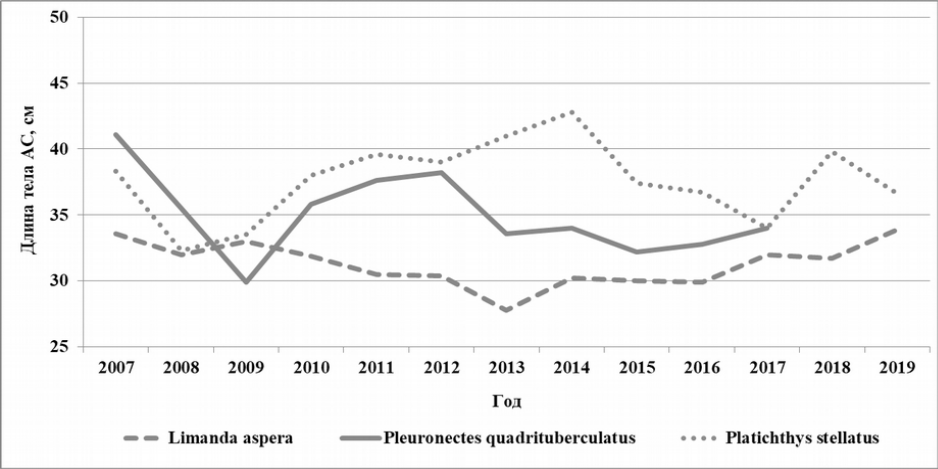
\includegraphics[width=0.9\textwidth]{authors/Byrlak-fig1.png}
  \end{center}
  \caption{Динамика средней длины тела АС (см) камбал из исследовательских уловов в северной части Охотского моря}
  \label{fig:byrlak-fig1}
\end{figure}

\begin{figure}[h!]
  \begin{center}
    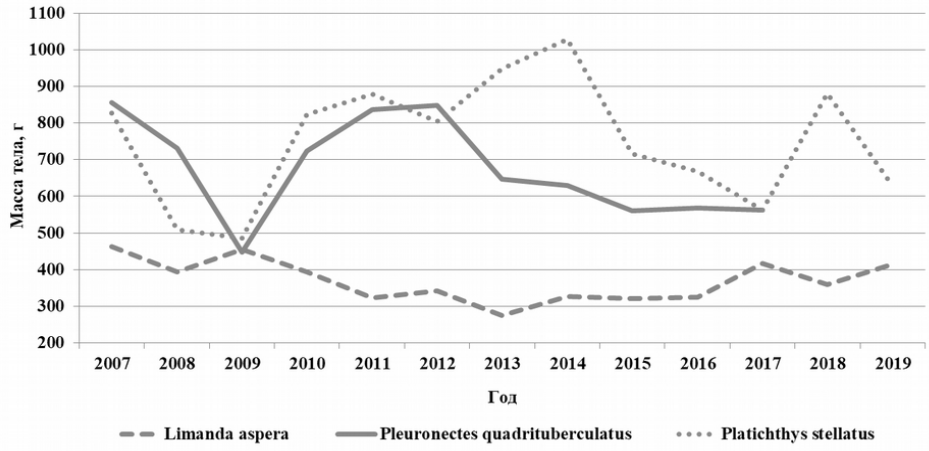
\includegraphics[width=0.9\textwidth]{authors/Byrlak-fig2.png}
  \end{center}
  \caption{Динамика средней массы тела (г) камбал из исследовательских уловов в~северной части Охотского моря}
  \label{fig:byrlak-fig2}
\end{figure}

\begin{figure}[h!]
  \begin{center}
    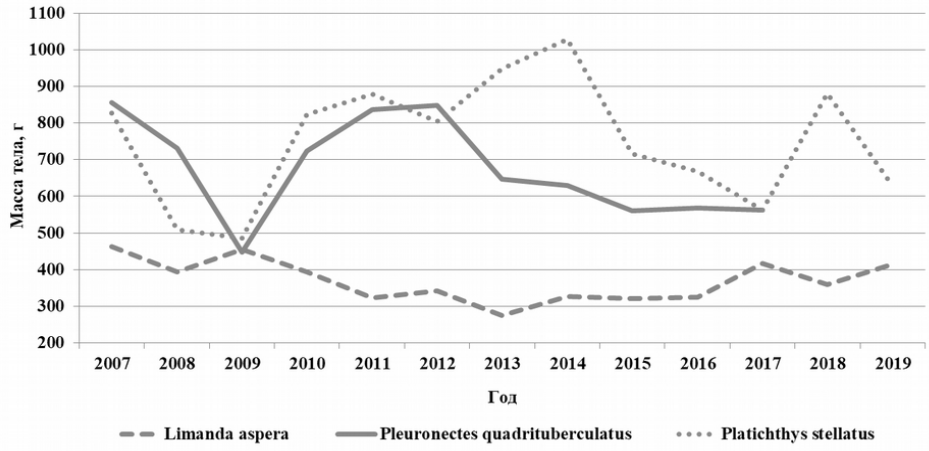
\includegraphics[width=0.9\textwidth]{authors/Byrlak-fig2.png}
  \end{center}
  \caption{Динамика среднего возраста (лет) камбал из исследовательских уловов в~северной части Охотского моря}
  \label{fig:byrlak-fig3}
\end{figure}

\begin{figure}[h!]
  \begin{center}
    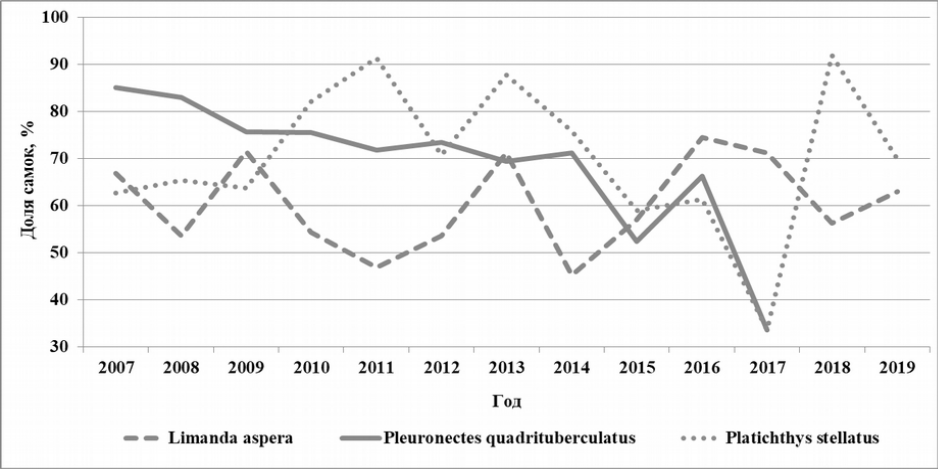
\includegraphics[width=0.9\textwidth]{authors/Byrlak-fig4.png}
  \end{center}
  \caption{Динамика доли самок камбал из исследовательских уловов в северной части Охотского моря}
  \label{fig:byrlak-fig4}
\end{figure}


В динамике средней длины и массы тела желтоперой камбалы (рис.~1, 2) в последние годы наблюдается незначительный подъем показателей, возможно, связанный с увеличением доли самок в уловах (рис. 4), которые крупнее самцов [1]. В то же время наблюдается снижение значения среднего возраста рыб (рис. 3).

Желтобрюхая камбала в исследовательских уловах 2018 и 2019~гг. не~наблюдалась. Начиная с 2012~г., наблюдается снижение средних биологических показателей, таких как размер, масса и доля самок (рис. 1, 2, 4).

У звездчатой камбалы наблюдается возрастание доли самок и снижение среднего возраста рыб (рис. 3, 4), что косвенно может являться индикатором вступления в промысел урожайного (высокочисленного) пополнения, т.\,к. пресс промысла на этот объект не значителен.

В целом, за период активного промышленного лова, в последние годы в~уловах, по нашим данным, наблюдаются скачки в средних биологических показателях для всех исследуемых видов камбал. Периодическое появление в уловах значительного количества мелких особей может свидетельствовать о чрезмерном прессе промысла, но, с другой стороны, и о возможном урожайном (высокочисленном) пополнении. Данные предположения нуждаются в дополнительных подтверждениях, по результатам комплексных донных съемок, которые необходимо выполнять в периоды различной активности рыб.

Поскольку промысел камбал приурочен к летнему периоду (в период большей пищевой и нерестовой активности) следует учитывать и такой фактор, как их слабая миграционная активность. Ошибочным будет мнение о~повсеместной большой плотности камбал в данный период, т.\,к. нерестовые и нагульные скопления локализированы только на определенных акваториях. За период 2015--2019~гг. суммарный среднегодовой вылов желтоперой (которая доминирует в уловах), желтобрюхой и звездчатой камбал составил 165,2\,\% от рекомендованного, при колебаниях от 76,6\,\% в 2015~г. до 300,7\,\% в 2019~г.


Такой чрезмерный вылов камбал, который в последние годы локализирован в небольших районах Тауйской губы и примыкающих к ней участках Притауйского района, до зал.~Бабушкина, может негативно сказаться на состоянии численности и биомассы этих видов в целом.


\begin{thebibliography}{99}

\bibitem{}
\BibAuthor{Дьяков~Ю.\,П.} Размерно-половая и половозрастная структура популяций дальневосточных камбал // Известия ТИНРО.~--- 2014.~--- Т.~177.~--- С.~78--109.
\bibitem{}
\BibAuthor{Семенов~Ю.\,К., Смирнов~А.\,А., Елатинцева~Ю.\,А., Ткаченко~А.\,А.} Особенности промысла донных рыб в 2019~г. в северной части Охотского моря // Рыбное хозяйство.~--- 2020.~--- №~2.~--- С.~43--50.
\bibitem{}
\BibAuthor{Черешнев~И.\,А., Волобуев~В.\,В., Хованский~И.\,Е., Шестаков~А.\,В.} Прибрежные рыбы северной части Охотского моря.~--- Владивосток~: Дальнаука, 2001.~--- 197~с.
\bibitem{}
\BibAuthor{Юсупов~Р.\,Р., и др.} Структура улова, состояние и промысел донных рыб в Северо-Охотоморском промысловом районе и зал. Шелихова Охотского моря  // Отчётная сессия ФГУП <<МагаданНИРО>> по результатам научных исследований 2011~г.: материалы докладов / Авт. Р.\,Р.~Юсупов, Ю.\,К.~Семенов, Л.\,П.~Николенко, А.\,И.~Каика, М.\,В.~Ракитина, А.\,С.~Сергеев, А.\,Ю.~Немченко, Ю.\,В~Сидяков.~--- Магадан~: МагаданНИРО. 2012.~--- С.~103--107.
\bibitem{}
\BibAuthor{Юсупов~Р.\,Р., Семенов~Ю.\,К., Шилин~Ю.\,А.} Рост и продукция массовых видов камбаловых рыб (Pleuronectidae) северной части Охотского моря // Исследования водных биологических ресурсов Камчатки и северо-западной части Тихого океана. Сб. науч. тр. Камчат. НИИ рыб. хоз-ва и океанографии.~--- 2015.~--- Вып.~36.~--- С.~14--24.
\end{thebibliography}

\procTitle{К лихенофлоре острова Спафарьева}
\procAuthor{Желудева~Е.\,В.}
\procEmail{elena.zheludeva.88@mail.ru}
\procOrganization{ИБПС ДВО РАН} \procCity{Магадан}

\makeProcTitle
\index{j@Желудева~Е.\,В.}

Изучение биоразнообразия и оценка его богатства~--- одна из важнейших задач современности. Без знания видового состава лишайников, играющих значительную роль в сложении растительного покрова, невозможно решать проблемы охраны природы и рационального использования растительных ресурсов.

Лишайники относятся к одной из наиболее широко распространённых групп организмов на территории Магаданской области. Они господствуют в напочвенном покрове большинства растительных сообществ. Несмотря на это, лихенофлора Магаданской области изучена весьма слабо и неравномерно. Проводившиеся ранее исследования касались, главным образом, её континентальной горной части (Тенькинский р-н) [1, 7; 9--11] и~охватывали, в~основном, напочвенные и эпилитные виды. По южной части области имеются лишь отрывочные сведения о лишайниках [13, 16, 20]. В~настоящее время начато планомерное изучение лихенофлоры Северо-Восточного Приохотья и~остров Магаданской области [3--7, 12].

Остров Спафарьева представляет собой два горных массива, соединенных низким пес\-ча\-но-галечным перешейком шириной от 300 до 600~м и длиной около 1~км. Площадь северного массива составляет около 22~км$^2$, южного~--- 10~км$^2$. Рельеф острова низкогорный: эрозионно-денудационные склоны сочетаются с узкими трогами и долинами ручьёв. Поверхность плато полого наклонена и осложнена останцами и нагорными террасами. Наивысшая точка южного массива~--- г.~Мыс Кактина, 313,5~м н.~у.~м., северного~--- г.~Командора Беринга, 572~м н.~у.~м.

Климат на острове (по данным метеостанций) характеризуется как приморский субарктический, с избыточным увлажнением, холодным летом и~снежной зимой. На о.~Спафарьева были найдены лишь несколько единичных экземпляров лиственницы кустовидной и~стланиковой форм. Каменноберезняки на о.~Спафарьева (северный массив) произрастают по~приморским склонам северо-северо-западной экспозиции, защищённым горами от ветров южных направлений. На южной части острова каменная берёза так же, как и~лиственница, представлена лишь несколькими экземплярами стланиковой или кустовидной формы. Крупные кустарники на о.~Спафарьева так же, как и~каменная берёза, предпочитают склоны, защищенные от юго-западных ветров, но распространены они несколько шире и образуют во многих случаях полукольцо, окружающее каменноберезовые рощи с трёх сторон (сверху, справа и слева). Особенностью южного массива о.~Спафарьева являются распространенные на пологих склонах и плато кустарниково-кустарничковые сообщества (0,1--0,5~м высотой) из стелющейся \textit{Duschekia fruticosa} (Rupr.) Pouzar, вересковых кустарничков и других видов, характерных для кустарничковых тундр, а также \textit{Boschniakia rossica} Chamisso et Sehlechtendal. Тундровая растительность занимает вершинные плато на~о.~Спафарьева (южн.), верхние части склонов, водоразделы и~гребни гор, переходит на~пологие склоны и днища долин. Для тундровой растительности характерно содоминирование кустарничков в различных соотношениях с лишайниками, мхами, осоками и травами. Лишайниково-кустарничковые (включая щебнистые и каменистые) тундры характерны для~верхних частей склонов, щебнистых и каменистых водоразделов. Каменистые и щебнистые фрагменты занимают 20--70\,\% поверхности [18].
\clearpage

\begin{table}[h!]
\caption*{\textbf{Таксономическая структура лихенофлоры класса \textit{Lecanoromycetes} о.~Спафарьева}}
\label{tab:zhelydeva}
\begin{tabular}{lllcc}
   \toprule
Подкласс          & Порядок                  & Семейство                 &  \parbox[c][4em][c]{0.1\textwidth}{ \centering Кол-во родов} & \parbox[c][4em][c]{0.1\textwidth}{ \centering Кол-во видов} \\
 \midrule
Lecanoromycetidae & Lecanorales              & \textit{Cladoniaceae}     & 1                & 19               \\
                  &                          & \textit{Parmeliaceae}    & 11                & 23               \\
                  &                          & \textit{Ramalinaceae}     & 1                & 3                \\
                  &                          & \textit{Stereocaulaceae}  & 1                & 2                \\
                  &                          & \textit{Sphaerophoraceae} & 1                & 2                \\
                  & Peltigerales             & \textit{Nephromataceae}   & 1                & 3                \\
                  &                          & \textit{Peltigeraceae}    & 1                & 8                \\
                  &                          & \textit{Lobariaceae}      & 1                & 1                \\
                  & Rhizocarpales            & \textit{Rhizocarpaceae}   & 1                & 1                \\
                  & Teloschistales           & \textit{Teloschistales}   & 1                & 1                \\
 \midrule
Ostropomycetidae  & Pertusariales            & \textit{Porpidiaceae}     & 1                & 1                \\
                  &                          & \textit{Icmadophilaceae}  & 2                 & 2                \\
                  &                          & \textit{Ochrolechiaceae}  & 1                & 2                \\
 \midrule
Incertae sedis    & Umbilicariales           & \textit{Ophioparmaceae}   & 1                & 1                \\
                  &                          & \textit{Umbilicariaceae}  & 2                & 5                \\
 \midrule
Всего: 2          & 6                        & 15                        & 27               & 74\\
\bottomrule

\end{tabular}
\end{table}


Работа написана по материалам, собранным сотрудниками ИБПС ДВО РАН Сазановой~Н.~А. и Зеленской~Л.~А. на территории острова в 2018~г. Обработка материалов осуществлялась в лаборатории ботаники Института биологических проблем Севера ДВО РАН (ИБПС ДВО РАН, г.~Магадан). Собранный материал (более 100 образцов) определен с~использованием стандартных анатомо-морфологических методов, а также цветных реакций, принятых при изучении лишайников, с использованием Определителя лишайников СССР [14], Определителя лишайников России [15], а также монографии и~публикации по~отдельным таксономическим группам [2, 8, 19]. Номенклатура и систематическое положение большей части видов выверены по каталогу <<Список лихенофлоры России>> [17]. Гербарные образцы хранятся в Гербарии ИБПС ДВО РАН (MAG, г.~Магадан).

В результате проведённого исследования выявлено 74~вида лишайников (см. таблицу), относящихся к 27~родам, 15~семействам, 6~порядкам класса Lecanoromycetes. Согласно проведённому анализу, в ряду субстратных групп доминируют эпигеиды~--- 44 вида. Их разнообразие значительно выше, чем у эпилитов~--- 15~видов и эпифитов~--- 13~видов. Эпиксилы представлены 2~видами и существенно уступают доминирующим группам.

Среди биоморфологических форм преобладают листоватые лишайники~--- 38~видов, кустистые~--- 29~видов, накипные~--- 4~вида и шиловидные~--- 3~вида. На острове Спафарьева отмечен редкий вид \textit{Peltigera scabrosella} Holt.-Hartw. Он обитает на почве среди других лишайников под покровом кедрового стланика на склонах северо-западной экспозиции. Вид,~включённый в красную книгу Магаданской области [6].

\begin{thebibliography}{99}
\bibitem{}\BibAuthor{Андреев М.~П.} Лишайники стационара <<Абориген>> (Тенькинский район, Магаданской области) // Бот. журн.~--- 1978.~--- Т.~63, №~11.~--- С.~1626--1632.

\bibitem{}\BibAuthor{Домбровская А.~В.} Род \textit{Stereocaulon} на территории бывшего СССР. СПб~: Мир и семья-95, 1996.~--- 270~с.

\bibitem{}\BibAuthor{Желудева Е.~В.} Первые данные о лишайниках Ямского участка заповедника <<Магаданский>>~// Вестник СВНЦ ДВО РАН.~--- 2012.~--- № 3.~--- С.~28--31.

\bibitem{}\BibAuthor{Желудева Е.~В.} Новые виды лишайников Магаданской области из Северо-Восточного Приохотья // Turczaninowia.~--- 2015.~--- Т.~18. №~4.~--- С.~5--15

\bibitem{}\BibAuthor{Желудева Е.~В.} Новинки лихенофлоры Магаданской области // Turczaninowia.~--- 2017.~--- Т.~20, №~2.~--- С.~64--74.

\bibitem{}\BibAuthor{Желудева Е.~В.} Лишайники // Красная книга Магаданской области. Редкие и находящиеся под угрозой исчезновения виды животных, растений и грибов. Магадан~: Охотник, 2019.~--- С.~301--312

\bibitem{}\BibAuthor{Журбенко М.~П.} Новые и редкие виды лишайников (Lichenes) из республики Саха-Якутия и~Магаданской области // Бот. журн.~--- 2003.~--- Т.~88. №~1.~--- С.~111--117.

\bibitem{}\BibAuthor{Заварзин А.~А.} К характеристике рода \textit{Peltigera} на территории России (предварительный список и ключ для определения таксонов) // Тр. Первой Рос. лихенолог. школы (Апатиты, 06–12.08.2000).~--- Петрозаводск~: Карельский науч. центр РАН. 2001.~--- С.~46--65.

\bibitem{}\BibAuthor{Королев Ю.~Б., Толпышева Т.~Ю.} Очерк флоры лишайников стационара <<Контакт>> (Верхнеколымское нагорье) // Новости систематики низших растений.~--- Л.~: Наука, 1980.~--- С.~137--149.

\bibitem{}\BibAuthor{Котлов Ю.~В.} Материалы к лихенофлоре Верхнеколымского нагорья // Новости систематики низших растений.~--- Л.~: Наука. 1995.~--- С.~66--72.

\bibitem{}\BibAuthor{Локинская М.~А.} Наиболее распространенные виды лишайников на Северо-Востоке СССР // Водоросли и грибы Сибири и Дальнего Востока.~--- Новосибирск~: Наука. 1970.~--- С.~233--245.

\bibitem{}\BibAuthor{Макрый Т.В., Желудева Е.~В.} Новые и редкие лишайники для Магаданской области // Turczaninowia.~--- 2012.~--- Т.~15. №~3.~--- С.~40--44.

\bibitem{}\BibAuthor{Окснер А.~Н., Блюм О.~Б.} К флоре лишайников Советского Дальнего Востока. I Сем. \textit{Peltigeraceae} // Новости систематики низших растений.~--- Л.~: Наука. 1971.~--- С.~249--263.

\bibitem{}Определитель лишайников России.~--- СПб.~: Наука, 1996.~--- Вып.~6.~--- 203~с.; 1998.~--- Вып.~7.~--- 166~с.

\bibitem{}Определитель лишайников СССР.~--- Л.~: Наука, 1971.~--- Вып.~1.~--- 412~с.; 1975.~--- Вып.~3.~--- 275~с.; 1978.~--- Вып.~5.~--- 305~с.

\bibitem{}\BibAuthor{Пярн А., Пааль Я.} Список лишайников // Исследования экосистем полуострова Кони (Магаданский заповедник) / А.~Лейто, Р.~Мянд, Т.~Оя, Я.~Паль, Т.~Тальви.~--- Таллин~: Изд-во Ак. Эстонии, 1991.~--- С.~16--18.

\bibitem{}\BibAuthor{Урбанавичюс Г.~П.} Список лихенофлоры России.~--- СПб.~: Наука, 2010.~--- 194~с.

\bibitem{}\BibAuthor{Хорева М.~Г.} Флора островов Северной Охотии.~--- Магадан~: ИБПС ДВО РАН, 2003.~--- 173~с.

\bibitem{}\BibAuthor{Чабаненко С.~И.} Обзор рода \textit{Hypogymnia} Российского Дальнего Востока // Тр. Первой Рос. лихенолог. школы (Апатиты, 06--12.08.2000).~--- Петрозаводск~: Карельский науч. центр РАН, 2001.~--- С.~265--276.

\bibitem{}\BibAuthor{Davydov E.~A., Zhurbenko M.~P.} Contribution to \textit{Umbilicariaceae} (lichenized Ascomycota) studies in Russia. l. Mainly arctic species // Herzogia.~--- 2008.~--- Vol.~21.~--- Р.~157-166.

\end{thebibliography}


\procTitle{Коллекция чешуекрылых в
фондах Магаданского областного краеведческого музея}

\procAuthorI{Тридрих~Н.\,Н.}
\procEmailI{tridrih\_nik@mail.ru}
\procOrganizationI{ИСИЭЖ СО РАН}
\procCityI{Новосибирск}

\procAuthorII{Кораблёва~Н.\,С.}
\procEmailII{nina-1112@mail.ru}
\procOrganizationII{МОКМ}
\procCityII{Магадан}

\makeProcTitleII
\index{t@Тридрих~Н.\,Н.}
\index{k@Кораблёва~Н.\,С.}


Алексей Петрович Васьковский родился 18 июня 1911\,г. в Ленинграде, умер в 16 августа 1979\,г., похоронен на Марчеканском кладбище. В 1930\,г. он поступает учиться на курсы младшего геологического персонала при институте цветных металлов Главного геолого-разведочного управления \mbox{(ГГРУ)}. С 1931\,г. он выезжает на Колыму в составе II\,Колымской экспедиции под руководством Юрия Александровича Билибина, и до 1933\,г. работает старшим коллектором, затем начальником партии. С 1933 по 1937\,г. от Дальстроя работает геологом-петрографом в сводной группе и одновременно учится в Ленинградском горном институте по специальности геолог. С 1937 по 1941\,г. работает в Индигирской геологоразведочной экспедиции, сначала начальником группы рудно-поисковых партий, потом начальником геолого-поискового отдела Индигирского геологоразведочного управления, а с 1939\,г.~--- главный геолог экспедиции. В этот период работы сделал свое первое открытие россыпного месторождения золота Туора-Тас, на базе которого впоследствии работал один из крупнейших приисков Дальстроя <<Ольчан>>.

Зимой 1942\,г. в блокадном Ленинграде, в очень трудных условиях, сдаёт государственные экзамены в институте и получает диплом 1-й степени (с~отличием) и выезжает на Колыму. С этого времени работает в геологоразведочном отделе Дальстроя начальником научно-исследовательского отдела. В 1949\,г. Алексей Петрович назначен начальником отдела сводных карт.%TODO: 1-й степени - может словами

В 1972--1979\,гг. заведовал лабораторией ландшафтоведения и охраны природы в Институте биологических проблем Севера.

Будучи профессиональным геологом и учёным с широким кругозором, он занимался исследованиями в различных областях геоморфологии, металлогении, формировании россыпных месторождений полезных ископаемых, стратиграфии и палеонтологии, истории четвертичного периода, как редактор и автор возглавлял работы по созданию обобщающих геологических, геоморфологических и стратиграфических карт Северо-Востока России и Арктики. Является автором более 80 печатных работ и 18 изданных геологических карт Северо-Востока России.

Другое яркое направление научных интересов и исследований Васьковского Алексея Петровича было связано с изучением живой природы Севера (флоры, фауны, почв), а также географии ландшафтов. В 1968\,г. Владимир Иванович Горазеев, руководитель областной секции озеленения Магаданского областного отделения Всероссийского общества охраны природы, в~комитет по радиовещанию и телевидению Магаданской области прислал предложение о введении раздела «Природа родного края» при этом советовал пригласить для участия Васьковского Алексея Петровича. В документе, присланном в комитет, он так написал о Васьковском: <<\textit{\mbox{...Он~--- геолог,} но\,хорошо знает нашу растительность и человек с большим кругозором...}>> [8].

Много лет А.\,П.\,Васьковский, помимо своей работы, занимался фенологией нашего края, публиковал брошюры «Ход сезонных явлений в окрестностях города Магадана» с результатами наблюдений, а\,также публиковал статьи с данными исследованиями в «Краеведческих записках Магаданского областного краеведческого музея».

В 1973\,г. вышла его брошюра <<Состояние охраны природы в Магаданской области>>. В ней он подробно описывает отрицательные последствия периода освоения области, а также все недостатки и просчёты в охране природы, обращает внимание на отсутствие заповедной зоны: <<\textit{...необходимо отметить, что Северо-Восток, ландшафты и биоценозы которого так интенсивно разрушались, не имеет на своей территории на одного заповедника и национального парка, охраняющего природу...}>> и указывает на необходимость выбора территорий, подлежащих охране с целью сохранения характерных ландшафтов и редких видов растений и животных, а~также организации заповедников и национальных парков на территории Магаданской области. И уже в 1974\,г. он выступает с инициативой создания заповедника <<Магаданский>>.

За открытие крупных месторождений полезных ископаемых и научный вклад в изучение Северо-Востока А.\,П.\,Васьковский был награждён орденом Ленина, орденами <<Красной Звезды>>, <<Знак почёта>>, а также медалями и значками [2].

В 1990\,г. в фонды музея Людмилой Ивановной Пастуховой, женой Алексея Петровича, была передана коллекция бабочек. Коллекция чешуекрылых собрана в окрестностях г.\,Магадана в период с 6 июля по 5 августа 1965\,г. и насчитывает 22 экземпляра. Коллекция представлена 16 видами бабочками из 7 семейств. Определением видового состава коллекции в 1967\,г. занимался Алексей Иванович Куренцов (1896--1975). Им определено 14 видов.
Алексей Иванович выдающийся биолог, энтомолог и биогеограф, доктор биологических наук, профессор, Заслуженный деятель науки РСФСР, лауреат Государственной премии СССР, основатель дальневосточной школы энтомологов.

В 1932\,г. переехал на Дальний Восток и посвятил изучению природы его территории почти 50 лет. В более чем 80 экспедициях обследовал территории Приморского и Хабаровского краёв, Амурской, Сахалинской, Камчатской, Магаданской, Читинской областей, Чукотского и Корякского\,АО, Якутии, Курильские острова. Исследовал речные долины Амура, Хора, Большой Уссурки, Бикина, горных рек и ручьёв, склоны Сихотэ-Алиня, хребты Джугджур и Яблонового, Колымское нагорье.

А.\,И.\,Куренцов занимался насекомыми~--- вредителями лесных насаждений. Основное внимание он уделял жукам, особенно короедам. Но, любимыми насекомыми Алексея Ивановича были бабочки. Во время первого своего путешествия на Дальний Восток в 1920\,г., он посвятил изучению этой группы более 40 работ, а монография <<Булавоусые чешуекрылые Дальнего Востока СССР>>, богато иллюстрированная цветными рисунками и картами ареалов, сразу же стала библиографической редкостью. В течение всей жизни Алексей Иванович в теоретических исследованиях постоянно возвращался к бабочкам для иллюстрации положений и выводов [4].
\enlargethispage{\baselineskip}

Нами была переэтикитирована коллекция с учётом современной систематики. Наибольший научный интерес в коллекции представляет \textit{Parnassius stubbendorfi}. Впервые в Магаданской области встреча с бабочкой \textit{Parnassius stubbendorfi} (Аполлон Штуббендрофа) \textit{Menetries}, 1849, была описана О.\,Э.~Костериным [3, 5] в 1992\,г. по результатам экспедиции на п-ов\,Кони в 1989\,г. Было поймано всего пару экземпляров, и эта находка сразу стала жемчужиной экспедиции. Дело в том, что впервые данный вид был отмечен на 59 параллели, что является самой крайней северной точкой ареала. Подвид магаданских Парусников Штуббендрофа получил имя О.\,Э.\,Костерина, и звучит как <<\textit{Parnassius stubbendorfi kosterini}>>. Отмеченная популяция встречается на Ольском участке заповедника <<Магаданский>>. До 2019\,г. в Магаданской области бабочка имела статус 3\,категории краснокнижной, как узкоареальный подвид североазиатского вида, представленный в области популяцией, вероятно реликт климатического оптимума голоцена [1]. В настоящее время \textit{Parnassius stubbendorfi} исключен из списка охраняемых видов и не вошёл во второе издание Красной книги Магаданской области. Основанием для исключения послужили новые сведения о распространении и численности, которые выявили отсутствие опасений о состоянии популяций на территории области.

Длина переднего крыла 25--30\,мм. Крылья белые с контрастными чёрными жилками. На передних крыльях самцов имеются две отчётливых сероватых (полупрозрачных) перевязи у внешнего края и узкое дискальное пятно. У самок эти элементы рисунка в среднем шире и более размытые [1, С.\,10]. Бабочка имеет бореальный сибирско-дальневосточный ареал. В нашей стране бабочка встречается в Среднесибирском, Южно-Западносибирском, Красноярском, Предалтайском, Горно-Алтайском, Тувинском, Прибайкальском, Прибайкальском, Забайкальском, Северо-Охо\-то\-морс\-ком, Средне-Охотоморском, Средне-Амурском, Нижне-Амурском и Приморском регионах [6].

В 2018\,г. данная коллекция чешуекрылых в составе материалов А.\,П.\,Вась\-ковского, в которые входили предметы палеонтологии, орнитологии, а также личные вещи, была принята на постоянное хранение в фонды Магаданского областного краеведческого музея.

\textbf{Аннотированный список видов.}

В описании видов после видового названия идёт: дата сбора; место сбора; количество экземпляров в коллекции; биотопическая приуроченность; ареал [7]; примечания.
\vspace{-6pt}
\begin{center}
\textbf{Класс Insecta (Насекомые)}

\textbf{Отряд Lepidoptera (Чешуекрылые)}
\end{center}

\textcenter{Семейство \textit{\MakeUppercase{Arctiidae}}~--- Медведицы}
\vspace{-8pt}
\begin{enumerate}[noitemsep, leftmargin=0cm]

      \item \textit{Setina irrorella insignata} (Staudinger, 1881)~--- 06.07.1965~г. Окрестности Магадана; 1 экземпляр; на приморских склонах, на лугах на границе леса на высоте около 1000 м над уровнем моря.

\textcenter{Семейство \textit{\MakeUppercase{NOCTUIDAE}}~--- Совки}

      \item \textit{Syngrapha} af. \textit{transbaicalensis} (Staudinger, 1892)~--- 06.07.1965~г. Окрестности Магадана; 1 экземпляр; в лиственничниках, на торфяниках, верховых болотах; бореальный сибирско-дальневосточный.

      \item \textit{Rhyacia ledereri} (Erschoff, 1870)~--- 06.07.1965~г. Окрестности Магадана; 2~экземпляра; на приморских склонах, в лиственничниках; бореальный восточнопалеарктический. Cиноним \textit{Agrotis ipsilon} (Hufnagel, 1766).

      \item \textit{Agrotis characteristica} (Alpheraky, 1892)~--- 06.07.1965 г. Окресности Mагадана; 3 экземпляра; степные биотопы. Синоним \textit{Agrotis robusta} (Eversmann, 1856).

\textcenter{Семейство \textit{\MakeUppercase{Hesperiidae}}~--- Толстоголовки}

      \item \textit{Carterocephalus palaemon} (Pallas, 1771)~--- 16.07.1965~г. Окрестности Магадана; 1 экземпляр; в долинах смешанных лесов и редколесьях; полизональный (кроме Арктики) голарктический.

      \item \textit{Carterocephalus silvicola} (Meigen, 1828)~--- 16.07.1965~г. Окрестности Магадана; 1 экземпляр; на приморских склонах, морях, полянах, реже в лиственничниках с березой, горных тундрах; полизональный (кроме Арктики) транспалеарктический.

\textcenter{Семейство \textit{\MakeUppercase{papilionidae}}~--- Парусники}

      \item \textit{Parnassius phoebus} (Fabricius, 1793)~--- 06.07.1965~г. Окрестности Магадана; 3 экземпляра; на травяных склонах, болотах, в горных тундрах; арктобореальный бореомонтанный голарктический.

    \item \textit{Parnassius stubbendorfi} (Menetrie, 1848)~--- 06.07.1965~г. Окрестности Магадана; 1 экземпляр; на приморских склонах, на лугах, в лиственничных редколесьях; бореальный сибирско-дальневосточный.

\textcenter{Семейство \textit{\MakeUppercase{Pieridae}}~--- Белянки}

      \item \textit{Colias palaeno} (Linnaeus, 1761)~--- 05.08.1965~г. Окрестности Магадана (р.~Каменушка); 1 экземпляр; в поймах, на лиственничных марях, в тундрах; арктобореальный циркумголарктический.

      \item Pontia callidice (Hubner, 1799)~--- 16.07.1965~г. Окрестности Mагадана; 1~экземпляр; на лугах, в горных, реже в низинных тундрах; арктобореальный арктоальпийский транспалеарктический. Синонимы \textit{Synchloe callidice} (Hubner, [1800]).

\textcenter{Семейство \textit{\MakeUppercase{Satyridae}}~--- Бархатницы}

      \item \textit{Coenonympha tullia} (Muller, 1764)~--- 05.08.1965~г. Окрестности Магадана (река Каменушка); 1~экземпляр и 16.07.1965~г. Окрестности Mагадана; 1~экземпляр; на болотах, в лиственничных редколесьях; полизональный циркумголарктический.

      \item \textit{Erebia ajanensis} (Menetries, 1857)~--- 06.07.1965~г. Окрестности Mагадана; 1~экземпляр; на приморских склонах, в лиственничных редколесьях; бореальный дальневосточный.

      \item  \textit{Erebia embla} (Thunberg, 1791)~--- 06.07.1965~г. Окрестности Магадана; 1~экземпляр; на болотах, марях, лиственничниках; арктобореальный транспалеарктический.

      \item \textit{Oeneis magna} (Graeser, 1888)~--- 16.07.1965~г. Окрестности Mагадана; 1~экземпляр; на лугах, болотах, в пойменных заболоченных и горных лиственничных редколесьях; бореальный сибирско-дальневосточный.

      \item \textit{Oeneis jutta} (Hübner, 1806)~--- 06.07.1965~г. Окрестности Магадана; 1 экземпляр; на лугах, болотах, в пойменных лесах, в заболоченных лиственничниках, лесотундрах и горных тундрах; субарктобореальный циркумголарктический.

\textcenter{Семейство \textit{\MakeUppercase{NYmphalidae}}~--- Переливницы}

      \item \textit{Boloria angarensis} (Ershov, 1870)~--- 05.08.1965~г. Окрестности Mагадана (р.~Каменушка); 1~экземпляр; на приморских склонах, лугах, болотах, в~лиственничных редколесьях, зарослях ольхи и кедрового стланика; арктобореальный палеарктический. Синоним \textit{Clossiana angarensis} (Ershov, 1870).
\end{enumerate}


\begin{thebibliography}{99}
%TODO: Оформить!

\bibitem{}\BibAuthor{Берман Д. И., Горбунов П. Ю., Катаев Б. М.} Красная Книга Магаданской области. Редкие и находящиеся под угрозой исчезновения виды растения и животных. – Магадан : ИБПС ДВО РАН, 2008. – 429 с.
\bibitem{}\BibAuthor{Васьковский А. П.} Состояние охраны природы в Магаданской области. – Магадан : ИБПС ДВНЦ АН СССР, 1973. – 10 с.
\bibitem{}\BibAuthor{Костерин О. Э.} Булавоусые чешуекрылые (Lepidoptera, Diurna) полуострова Кони. Магаданская область // Actias. – 1994. – № 1. – C. 77–81.
\bibitem{}\BibAuthor{Купянская А. Н., Лелей А. С., Стороженко С. Ю.} Алексей Иванович Куренцов // Вестник ДВО РАН. – 2007. – № 6. – С. 155–161.
\bibitem{}\BibAuthor{Лейто А., Мянд Р., Оя Т.} Исследование экосистем полуострова Кони. Магаданский заповедник. – Таллин: АН Эстонии, 1991. – 224 с.
\bibitem{}\BibAuthor{Рябухин А. С., Засыпкина И. А.} Наземные и пресноводные насекомые побережья Тауйской губы // Биологическое разнообразие Тауйской губы Охотского моря. – Владивосток : Дальнаука, 2005. – С. 290–476.
\bibitem{}\BibAuthor{Синев С. Ю., Козлов М. В.} Micropterigidae : каталог чешуекрылых (Lepidoptera) России. – СПб. ; М. : Т-во научных изданий КМК, 2008. – С. 296–423.

\textbf{Архивные источники}

\bibitem{}Предложение Горазеева В. И. комитету по радиовещанию и телевидению ввести раздел <<Природа родного края>> с привлечением геолога Васьковского А.П. и др. – Магадан, 1968. – 1 л. (из фондов Магаданского областного краеведческого музея).
\end{thebibliography}


%
\rasdel{Физико-математические и компьютерные исследования}
\procTitle{Оценка новизны решений в автоматизированной системе распределения грантов}
\procAuthor{Копченко~В.\,К.}
\procEmail{vkkopchenko49@gmail.com}
\procOrganization{СВГУ} \procCity{Магадан}

\makeProcTitleRazdel
\index{k@Копченко~В.\,К.}

В постиндустриальном обществе преобладает инновационный сектор экономики, в котором доминирует высокопроизводительная промышленность, связанная с информационными технологиями. Эти технологии обслуживают потребности государства, бизнеса, организуют социальное взаимодействие, осуществляют информационную поддержку здравоохранения, образования, культуры и иных государственных отраслей. Выделяют следующие наиболее значимые требования к данной области [1, 2]:
\begin{enumerate}[noitemsep]\vspace{-8pt}
      \item адаптацию к постоянно растущему объёму данных;
      \item обеспечение непрерывной работы информационного цикла;
      \item минимизацию ошибок.
\end{enumerate}\vspace{-8pt}

Выполнение данных требований невозможно без надлежащим образом осуществляемого управления на государственном уровне [3]. Например, для первых двух целей в рамках Стратегии развития информационного общества в Российской Федерации на 2017--2030\,гг. [17] было сформулировано направление развития российских информационных и коммуникационных технологий, содержательной основой которого является разработка и обеспечение использования электронно-компонентной базы и программных продуктов российского производства, а также нормативно-правовая и научная базы. Указ Президента РФ №\,490 [18] расширяет круг задач, решаемый интеллектуальными системами, в целях повышения эффективности процессов принятия управленческих решений и минимизации ошибок в таковых.

К последнему классу задач можно отнести распределение ресурсов на основе экспертных оценок в условиях многокритериальности и действующих ограничений, иначе называемое распределением грантов. Данный характер финансирования установлен Указом Президента РФ от 30.01.2019\,г. №\,30 <<О грантах Президента Российской Федерации, предоставляемых на развитие гражданского общества>> [19]. Грантовая система распределения основана на удовлетворении заявок на проектное финансирование. Подобные системы основаны на экспертных оценках, а в свете существующих технологий достойны применения соответствующих средств автоматизации, пренебрежение которыми снижает прозрачность экспертизы, создаёт предпосылки к предвзятому оцениванию в целях собственной выгоды экспертам [7].

В научной публицистике существуют работы, направленные на решение названных проблем. Существующие публикации можно условно разбить на три группы:
\begin{enumerate}[noitemsep]
  \item разработки, направленные на формализацию критериев, что позволит снизить влияние субъективных взглядов эксперта на результат анализа. Примерами таких работ выступают [9--11]. Несмотря на высокий уровень исследований, остаётся открытым вопрос выбора функции свёртки частных показателей, который в настоящее время не~решается научным сообществом;
  \item разработки, направленные на формирование экспертных пулов с учётом научно-технического профиля каждого эксперта с динамическим изменением показателей их компетенций в различных отраслях деятельности. Данные рассуждения приведены в работах [8, 12, 13]. Следует отметить, что увеличение числа экспертов увеличит затраты на расчёт вышеназванных метрик компетентности, что в большинстве случаев исключает возможность практического использования данного класса разработок;
  \item разработки,\;\;\;направленные\;\;на\;\;максимальную\;\;\;унификацию\;\;критериев\;\;оценивания без~учёта особенностей, связанных с отраслевой принадлежностью и форматом финансируемого объекта. Яркими примерами служат публикации [14--16]. Данные методы не~всегда могут быть применимы, так как у большинства грантооператоров категория применения проекта оценивается согласно перечню приоритетных отраслей экономики, который не поддаётся унификации ввиду отсутствия у многих видов деятельности общих характеристик.
\end{enumerate}

Несмотря на отсутствие готовых концептуальных решений, на основе дальнейшего анализа научных публикаций, в частности [17, 18], можно сделать вывод о сводимости экспертизы любой заявки на проектное финансирование к трём действиям: отраслевой идентификации, анализу уникальности и анализу новизны. Однако в настоящее время на рынке программных продуктов отсутствуют технические решения для проведения анализа заявки на получение гранта, включающие предложенный комплекс действий, в связи с чем было принято решение о разработке автоматизированной системы распределения грантов (АСРГ), концепция которой сформулирована в работе [19]. Организационно-процессная модель удовлетворения заявки $\Theta$ на грант с отметкой времени \textit{TO BE} представлена следующим кортежем:
\begin{equation}
  \Theta_{TO-BE} = \langle \Psi, P_p, M, Q_p, Q_M, O_M \rangle,
\end{equation}
где $\Psi$~--- множество заявок; $P_p$~--- множество процедур предварительной оценки; $M$~--- процедура экспертной оценки; $Q_p$~--- множество критериев для предварительной оценки; $Q_M$~--- множество критериев для экспертной оценки; $O_M$~--- множество численных оценок. В общем виде схему работы АСРГ можно описать Swimlane-диаграммой (рис.\,1).

Предварительная оценка определяет отраслевую принадлежность проекта согласно исследованию [20]. Величина \textit{r} соответствия заявки \textit{g}-й отрасли знания рассчитывается следующим образом:
\begin{equation}
  r = \text{max}\sum_{\text{c}\,=\,1}^{|\text{G}|}{w_{ij}},
\end{equation}
где G~--- множество отраслей, $\text{G}~= \{g_1, g_2,\dots, g_c \}$; c = |G|; $j=\overline{1,|g_i|}$; $w_{ij}$~--- вес \textit{j}-го терма в~\textit{i}-й отрасли. Термы и веса определены заранее и хранятся в базе данных системы. Данный метод был реализован в рамках конференции [21] и показал высокую эффективность.

Экспертная оценка включает в себя анализ заимствований в тексте заявки (плагиат) с~помощью алгоритма шинглов, эффективность которого рассмотрена в работе [22], и оценку новизны предлагаемого проекта. Для реализации данного функционала требуется формализация заявки. Заявка представлена в виде:
\begin{equation}
  R_{eq}= < F, C, V >,
\end{equation}
\enlargethispage{\baselineskip}


\begin{figure}[H]
  \begin{center}
    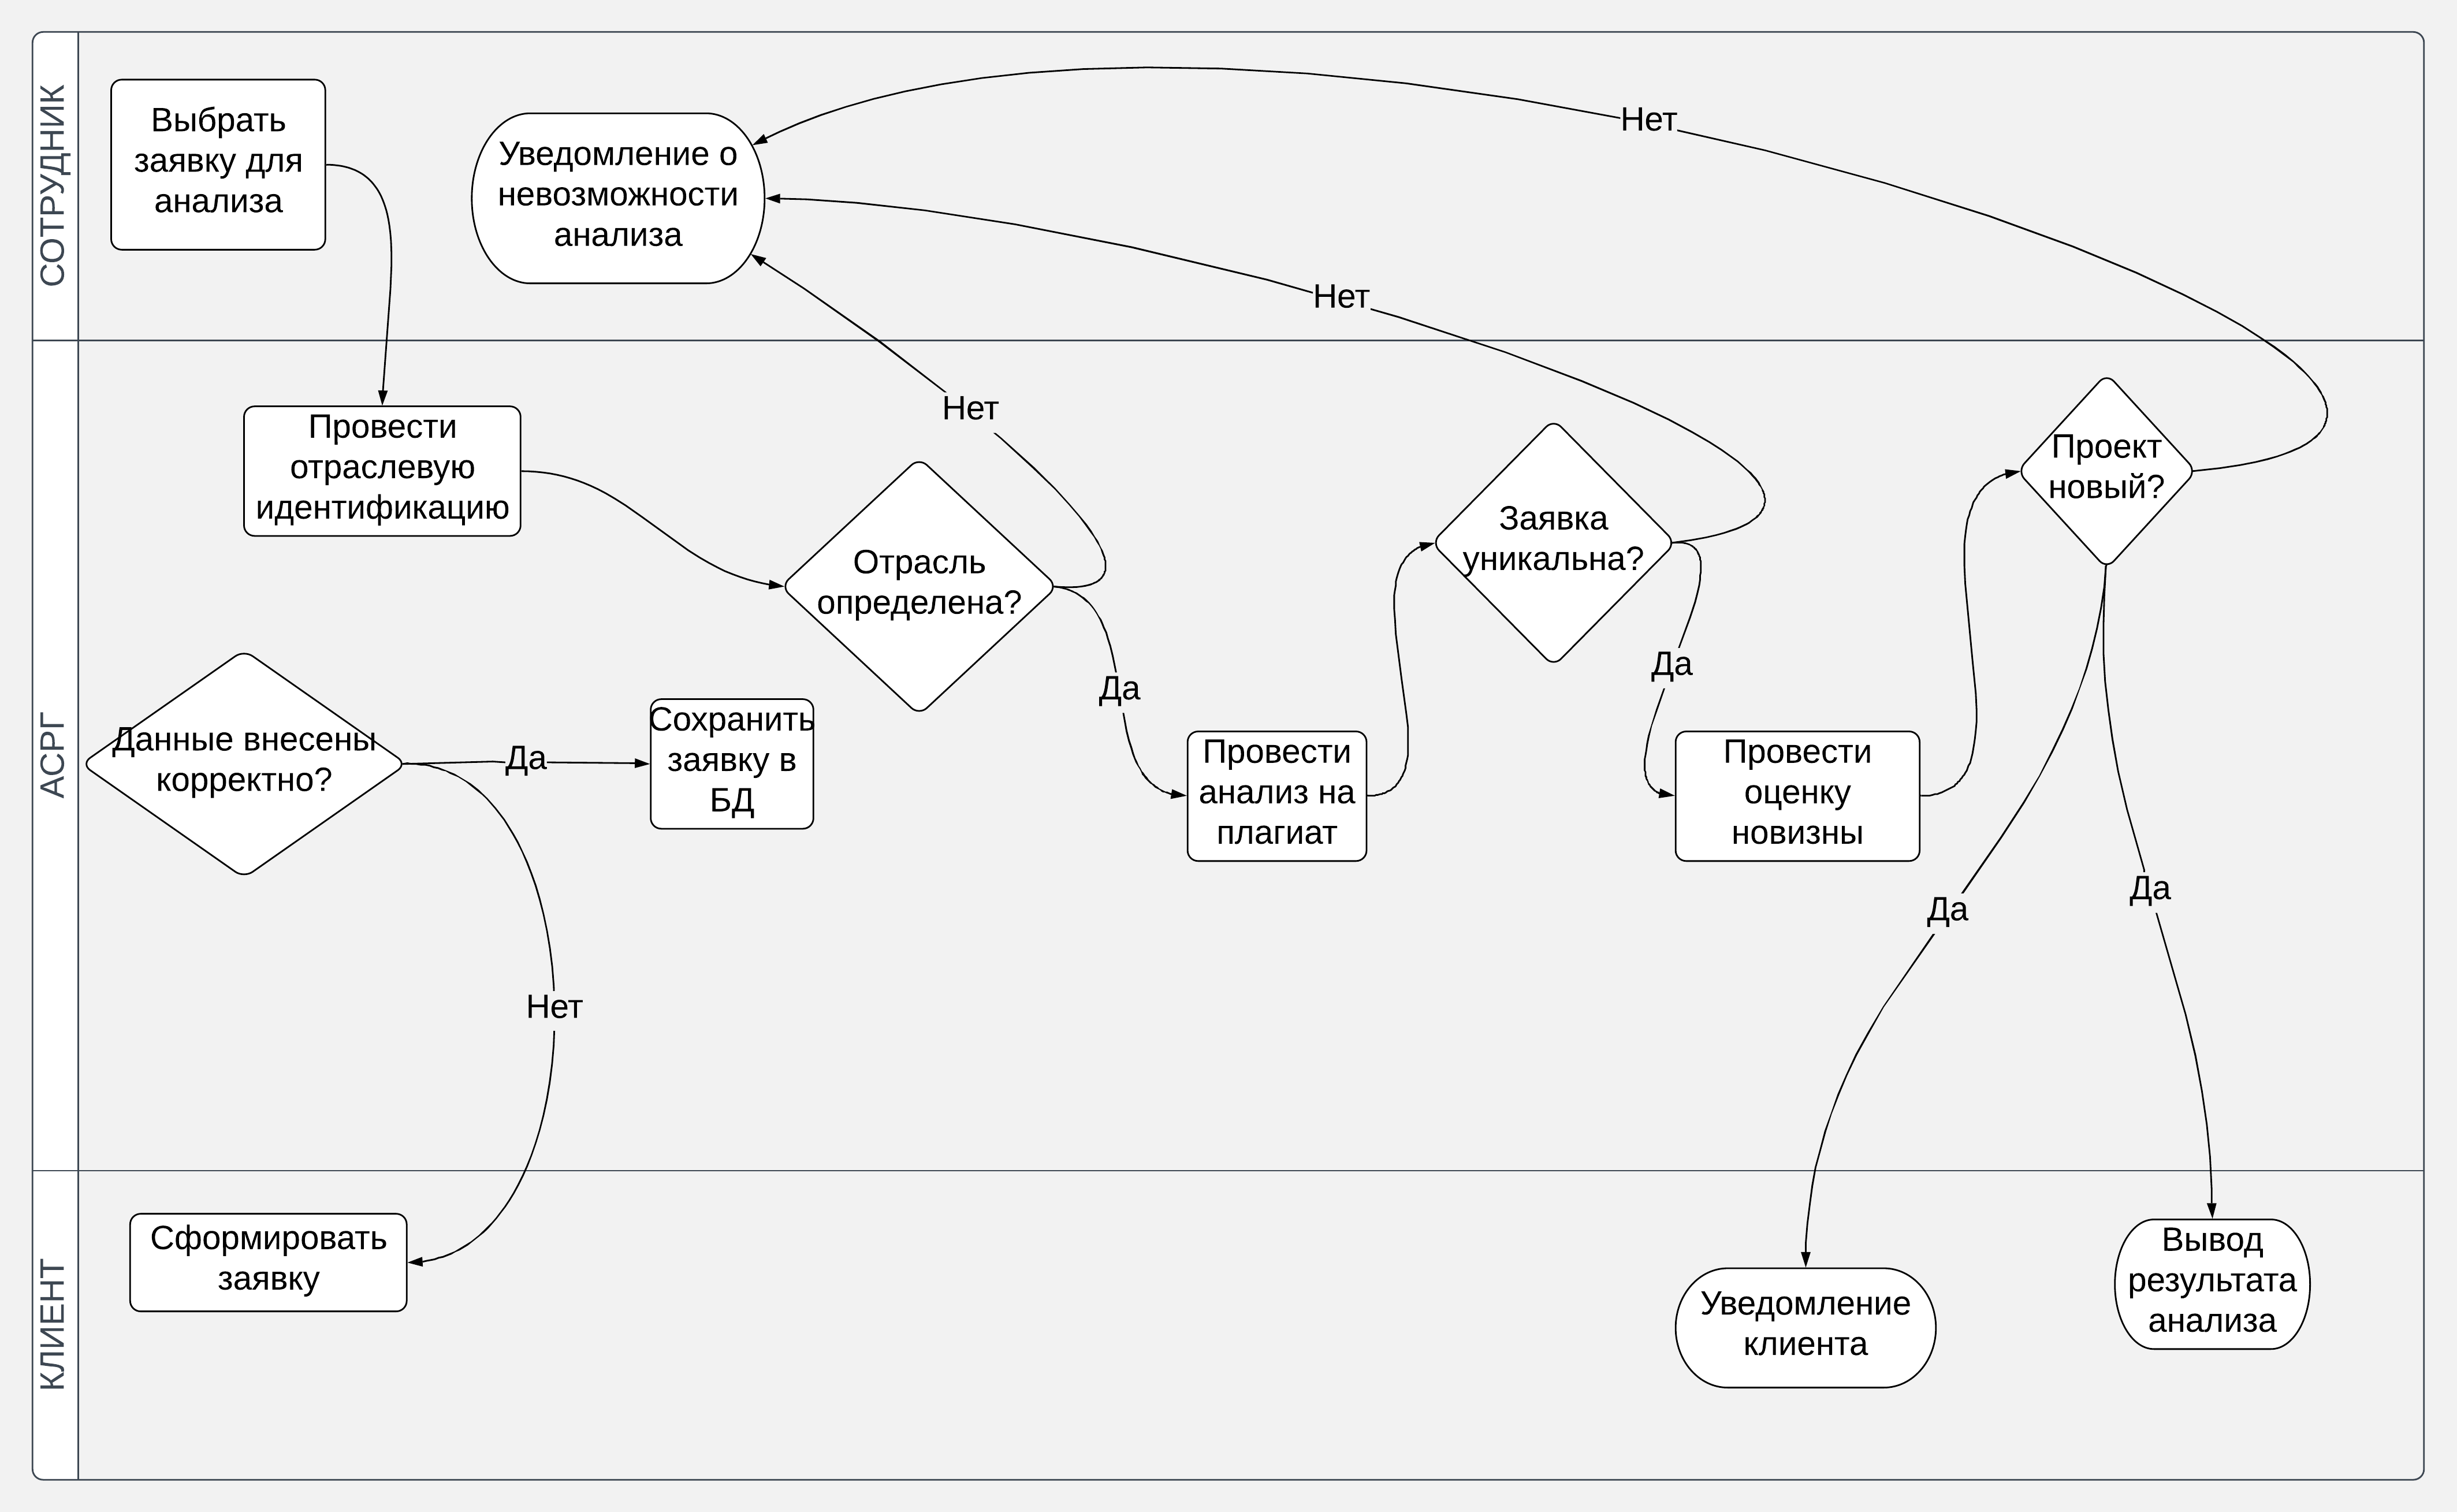
\includegraphics[width=1\textwidth]{authors/kopchenko-fig-1.png}
  \end{center}
  \caption {Swimlane-диаграмма экспертизы АСРГ}

\end{figure}



где \textit{F}~--- краткое описание проекта; \textit{C}~--- детальное описание проекта; \textit{V}~--- атрибуты заявки, определяемые АСРГ. Краткое описание представлено следующей структурой:
\begin{equation}
  F = < F_T, F_S, F_N >,
\end{equation}
где $F_T$~--- наименование проекта; $F_S$~--- краткое описание проекта общими признаками; $F_N$~--- признаки, обеспечивающие новизну решения. Атрибуты АСРГ сопровождаются кортежем:
\begin{equation}
  V = < I, U, H >,
\end{equation}
где \textit{I}~--- отрасль заявки; \textit{U}~--- уникальность заявки; \textit{H}~--- величина новизны проекта.

Оценку новизны можно разделить на три этапа:
\begin{enumerate}[noitemsep]\vspace{-8pt}
    \item поиск прототипа проекта;
    \item поиск отличий проекта от прототипа;
    \item оценка положительного эффекта.
\end{enumerate}\vspace{-8pt}

Прототипом можно считать заявку, у которой величина совпавших с текущей заявкой признаков новизны максимальна:
\begin{equation}
  d_i = \text{max} Sim_j,
\end{equation}
где $Sim_j = F_{N_i} \cap F_{N_j}$ количество совпадений признаков из перечня признаков новизны рассматриваемой \textit{i}-й заявки в списке новшеств документа из архива заявок \textit{Docs}, \textit{d}~--- прототип (заявка). В~случае отсутствия результата можно относительно рассматриваемого множества термов описательной части заявки \textit{С} сопоставить каждому признаку $k_i$ величину $w_i$, называемую весом. В~этом случае прототипом \textit{d} проекта, претендующего на грант, можно считать проект, удовлетворяющий выражению:
\begin{equation}
  d = arg\text{max} \sum_{k=1}^{|Docs|}w_{kj},
\end{equation}
где \textit{k}~--- терм в детальном описании проекта, \textit{w}~--- вес терма, $j=\overline{1,|C|}$.

Данный функционал АСРГ был реализован в виде WEB-приложения на языке php с~использованием WEB-сервера Apache и системой управления базами данных MySQL. Для~автоматизации работы с~действиями CRUD и установления базовой защиты была выбрана ORM-библиотека RedBeanPHP, которая отлично зарекомендовала себя как простое в~использовании средство с широким перечнем автоматических операций, вплоть до динамического изменения структуры таблиц и всей базы данных в целом при необходимости, причём прямого вмешательства разработчика в процесс не требуется. Информационная модель предметной области базы данных представлена на рис.\,2.

\begin{figure}[H]
  \begin{center}
    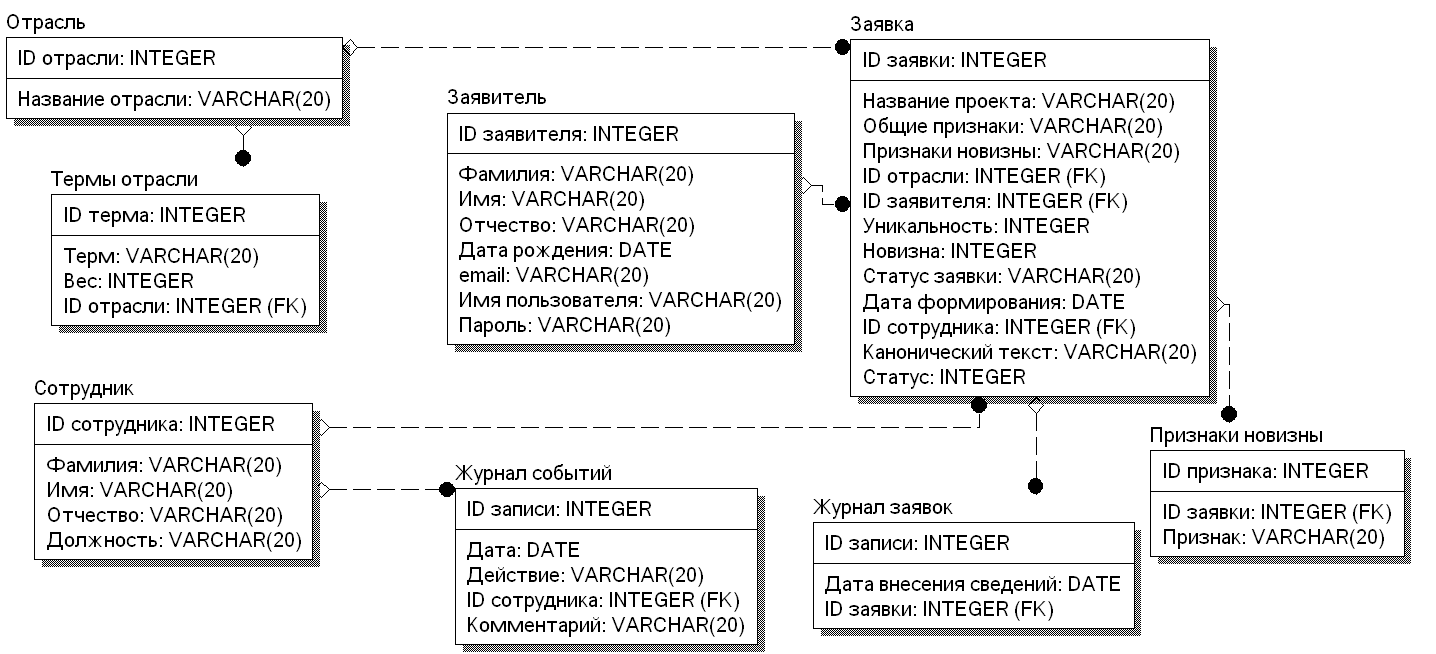
\includegraphics[width=1\textwidth]{authors/kopchenko-fig-2.png}
  \end{center}
  \caption {Информационная модель предметной области базы данных}

\end{figure}


В результате проведённых исследований был разработан программный модуль для оценки новизны проекта, претендующего на получение финансовой поддержки. Работа модуля включает в себя поиск прототипа предлагаемого решения и дальнейший терминологический анализ идентичности при наличии положительного результата. Реализованные средства АСРГ демонстрируют высокую эффективность в анализе отраслевой принадлежности, заимствований и оценке новизны, что предполагает дальнейшие исследования с целью разработки функции свёртки полученных показателей и автоматизации проведения конкурсной процедуры, что позволит минимизировать влияние личных предпочтений эксперта в~пользу объективности и скорости анализа заявки.


\begin{thebibliography}{99}
%1

\bibitem{}\BibAuthor{Васин С.\,Г.} Искусственный интеллект в управлении государством // Управление.~--- 2017.~--- №\,3 (17).~--- URL: https://cyberleninka.ru/\-arti\-cle/\-n/iskus\-stven\-nyy-intel\-lekt-v-up\-rav\-lenii-gosu\-dars\-tvom (дата обращения: 16.03.2020).

\bibitem{}\BibAuthor{Вендров\,А.\,М.} Проектирование программного обеспечения экономических информационных систем.~--- М.\,: Финансы и статистика, 2005.~--- 544\,с.

\bibitem{}\BibAuthor{Горчакова\,Е.\,А.} О необходимости унификации критерия отбора проектов кооперации промышленных предприятий в кластере // Известия СПбГЭУ.~--- 2017.~--- №\,5 (107).~--- URL: https://cyberleninka.ru/article/n/o-neobhodimosti-unifikatsii-kriteriya-otbora-proektov-kooperatsii-promyshlennyh-predpriyatiy-v-klastere (дата обращения: 20.02.2020).

\bibitem{}\BibAuthor{Ильин\,И.\,В.} Критерии отбора проектов для их эффективной реализации на условиях проектного финансирования // Финансы и кредит.~--- 2008.~--- №\,35 (323).~--- URL: https://cyberleninka.ru/article/n/kriterii-otbora-proektov-dlya-ih-effektivnoy-realizatsii-na-usloviyah-proektnogo-finansirovaniya-2 (дата обращения: 20.02.2020).

\bibitem{}\BibAuthor{Копченко\,В.\,К., Сироткин\,А.\,В.} Применение систем искусственного интеллекта для распределения грантов предпринимателям Магаданской области // Студенческий: электрон. научн. журн.~--- №\,11 (55).~--- С.\,20--24.

\bibitem{}\BibAuthor{Косоруков\,А.\,А.} Технологии искусственного интеллекта в современном государственном управлении // Социодинамика.~--- 2019.~--- №\,5.~--- С.\,43--58.~--- DOI: 10.25136/2409-7144.2019.5.29714

\bibitem{}III\,Международная научно-практическая конференция <<На перекрестке Севера и Востока (методологии и практики регионального развития)>> / Северо-Восточный государственный университет.~--- 2019.~--- URL: http://svkonf.svgu.ru (дата обращения: 21.02.2020).

\bibitem{}\BibAuthor{Марон~А.\,И., Марон~М.\,А.} Метод конкурсного отбора проектов // Открытое образование.~--- 2011.~--- №\,2.~--- URL: https://cyberleninka.ru/article/n/metod-konkursnogo-otbora-proektov (дата обращения: 20.02.2020).

\bibitem{}\BibAuthor{Мельник~П.\,Б.} Математическая постановка задачи формирования реестра экспертов // Инноватика и экспертиза.~--- 2014.~--- №\,2 (13).~--- С.~69--81.

\bibitem{}\BibAuthor{Мельник~П.\,Б.} Методика формирования экспертных пулов и групп для проведения экспертно-аналитических исследований // Там же.~--- 2017.~--- №\,1 (19).~--- С.\,39--54.

\bibitem{}\BibAuthor{Мельник~П.\,Б.} Реестр экспертов как система массового обслуживания: модель и параметры входящего потока заявок // Там же.~--- 2018.~--- №\,1 (22).~--- С.\,67--78.

\bibitem{}\BibAuthor{Морозова\,Т.\,В.} Экспертные технологии в оценке инновационных проектов // Известия ЮФУ. Технические науки.~--- 2011.~--- №\,11.~--- URL: https://cyberleninka.ru/article/n/ekspertnye-tehnologii-v-otsenke-innovatsionnyh-proektov (дата обращения: 20.02.2020).

\bibitem{}\BibAuthor{Новикова\,Т.\,Г.} Теоретические основы экспертизы инновационной деятельности в образовании~: автореф. дис. $\dots$ д-ра пед. наук.~--- Москва, 2006.~--- 47\,с.


\bibitem{}\BibAuthor{Семиглазов\,В.\,А.} Развитие методики отбора инновационных проектов в условиях полной неопределённости // Инновации.~--- 2006.~--- №\,11.~--- URL: https://cyberleninka.ru/article/n/razvitie-metodiki-otbora-innovatsionnyh-proektov-v-usloviyah-polnoy-neopredelennosti (дата обращения: 20.02.2020).

\bibitem{}\BibAuthor{Сироткин\,А.\,В., Копченко\,В.\,К.} Концепция разработки автоматизированной системы распределения грантов // EurasiaScience~: сб. статей XXI междунар. науч.-практ. конф.~--- М.\,: Науч.-издат. центр <<Актуальность.рф>>, 2019.~--- С.\,107--109.

\bibitem{}\BibAuthor{Сироткин\,А.\,В., Старикова\,О.\,А.} Отраслевая идентификация заявок в автоматизированной экспертной системе распределения грантов // Современные наукоёмкие технологии.~--- 2019.~--- №\,7.~--- С.\,99--103.

\bibitem{}Указ Президента РФ от 09.05.2017~г. №~203 <<О\,Стратегии развития информационного общества в Российской Федерации на 2017--2030 годы>>~// Консультант Плюс.~--- URL: http://www.consultant.ru/document/cons\_doc\_LAW\_216363/ (дата обращения: 16.03.2020).

\bibitem{}Указ Президента Российской Федерации от 10.10.2019~г. №~490 <<О развитии искусственного интеллекта в Российской Федерации>>~// Консультант Плюс.~--- URL: http://www.consultant.ru/document/cons\_doc\_LAW\_335184/ (дата обращения: 16.03.2020).

\bibitem{}Указ Президента РФ от 30.01.2019~г. №~30 <<О грантах Президента Российской Федерации, предоставляемых на развитие гражданского общества>>~// Законы, кодексы и нормативно-правовые акты в Российской Федерации.~--- URL: https://legalacts.ru/doc/ukaz-prezidenta-rf-ot-30012019-n-30-o-grantakh/\#100014 (дата обращения: 16.03.2020).


\bibitem{}\BibAuthor{Шушкевич~Н.\,А., Мохов~А.\,И., Крупский~А.\,Ю., Нургазиева~А.\,С.} Экспертиза проектов на основе информационной модели // Вестник евразийской науки.~--- 2010.~--- №\,4.~--- URL: https://cyberleninka.ru/article/n/ekspertiza-proektov-na-osnove-informatsionnoy-modeli (дата обращения: 20.02.2020).


\bibitem{}\BibAuthor{Ясенев\,В.\,Н.} Информационные системы и технологии в экономике~: 3-е изд., перераб. и доп.~--- М.\,: ЮНИТИ, 2012.~--- 560\,с.

\bibitem{}\BibAuthor{Broder\,A.} Identifying and Filtering Near-Duplicate Documents, COM’00 // Proceedings of the 11th Annual Symposium on Combinatorial Pattern Matching.~--- 2000.~--- P.\,1--10.
\end{thebibliography}
\thispagestyle{empty}

\procTitle{Инженерные уроки (разработка демонстрационных установок)}
\procAuthor{Лейбович~Е.\,О., Ус~Я.\,М., Магомедов~М.}
\procEmail{evgeniiamgdn@gmail.com, yanina4444@icloud.com, 05ru9479@gmail.com}
\procOrganization{СВГУ} \procCity{Магадан}

\makeProcTitle
\index{l@Лейбович~Е.\,О.}
\index{y@Ус~Я.\,М.}
\index{m@Магомедов~М.}

Количество абитуриентов, поступающих на технические специальности, в последние годы продолжает снижаться. Соответственно, отрасли инженерной деятельности испытывают недостаток новых кадров. В то же время на основании проведённых Московской школой управления <<Сколково>> и Агентством стратегических инициатив исследований до 2030\,г. предполагается появление 136 новых профессий, среди которых: архитектор энергонулевых домов, проектировщик дирижаблей, архитектор территорий, урбанист-эколог, инженер роботизированных систем и многие другие [1].

Таким образом, вопрос о повышении интереса современной молодёжи к инженерному направлению продолжает оставаться актуальным. В ближайшем и более далёком будущем однозначно останутся востребованы специалисты в области естественных наук и инженерии. А это значит, что надо заинтересовать детей уже младшего школьного возраста в изучении физики, химии, математики и астрономии.

В Северо-Восточном государственном университете на протяжении последних трёх лет реализуется проект научно-познавательной площадки <<Эврика>>, целью которого является организация работы со школьниками по вовлечению их в процесс активного познания мира. Студентами разработаны и проведены в школах города и области мероприятия, которые наглядными экспериментами знакомили школьников с основами естественных наук (в частности, физики). В ходе мероприятий детям позволяется самостоятельно проводить несложные и безопасные эксперименты.

Особенностью нового элемента нашей площадки является инженерное направление. Сейчас мы предлагаем для проведения познавательных мероприятий три новые установки, разработанные студентами политехнического института. Эти установки демонстрируют законы физики, лежащие в основе работы многих механизмов.

Основной нашей целевой аудиторией являются представители поколения Z. Но многие из участников наших больших мероприятий ещё недостаточно самостоятельны, и поэтому сопровождаются взрослыми~--- родственниками, учителями и т.\,п. Это могут быть как представители поколения Y, так и поколений X и даже <<беби-бумеров>> [2].

Можно иметь различные взгляды на теорию поколений, но тот факт, что понимание ценностей различных поколений позволяет подстраивать содержание мероприятий под интересы каждого, является неоспоримым и проверено нами на личном опыте. У каждого поколения свои ценности, но их объединяет одно~--- представители всех поколений готовы учиться, развивая себя. И готовы взаимно обмениваться своим опытом как со старшим, так и с младшим поколением.

Все созданные нами установки просты в своей конструкции и могут быть собраны самостоятельно. Они имеют различные степени сложности и набор деталей, но каждая из них демонстрирует универсальные законы природы, с которыми мы ежедневно сталкиваемся и в обычной жизни – закон сохранения импульса и закон сохранения энергии.

Первая установка позволяет проследить баллистическую траекторию движения (рис.1). Нам понадобятся две коробки небольшого размера и машинка. Одна из коробок ставится вертикально. К ней крепится ранее вырезанная из другой коробки рампа (направляющая лента), таким образом, чтобы дно рампы коснулось поверхности, на которой размещается установка.  К концу рампы присоединяем маленькую коробку, с помощью которой можно будет контролировать наклон рампы. Рядом с установкой строится карточный домик, который можно будет разбить машинкой. Наклоном рампы регулируется дальность полёта машинки. Спускающаяся по рампе машинка под действием сил набирает скорость, а наклон рампы обеспечивает её дальнейшей траектории баллистический характер. Такую форму движения имеет любое тело, брошенное под углом к горизонту и движущееся под действием силы тяжести. Например, межконтинентальные баллистические ракеты считаются таковыми, поскольку продолжают своё движение к цели после выключения двигателей, как раз по траектории, называемой баллистической. Таким образом, наша первая установка предназначена для проведения в домашних условиях экспериментов по исследованию баллистической траектории движения.

\begin{figure}[h!]
  \begin{center}
    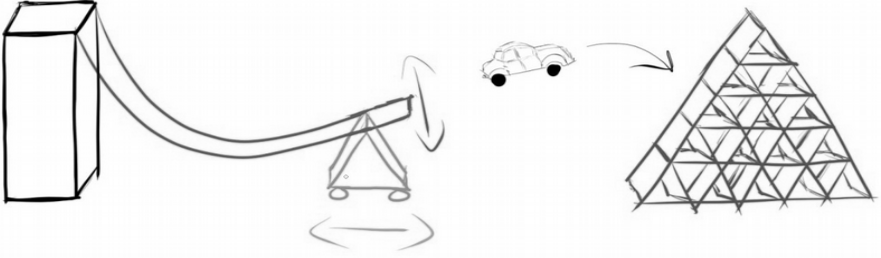
\includegraphics[width=0.7\textwidth]{authors/leybovich-fig1.png}
  \end{center}
  \caption{Схема установки <<Баллистика>>}
  \label{fig:leybovich-fig1}
\end{figure}


Вторая установка (рис. 2) демонстрирует законы сохранения энергии и перехода её из одного вида в другой (принцип <<домино>>). Вначале изготавливается каркас для направления движения шара по конструкции. Каркас конструируется из двух горок и двух горизонтально положенных досок. Первая часть установки состоит из стойки, с которой покатится шар, а также горки и доски, по которым шар покатится в мельницу. Мельница собирается из ножки (используемой как опора) и подставки (с помощью которой мельница будет держать устойчивое положение). Лопасти мельницы состоят из трёх лёгких перекрещенных дощечек, которые закреплены с помощью шурупа. Шуруп крепится к моторчику, который будет вращать лопасти мельницы. Вторая часть у состоит из доски, по которой шар скатывается с мельницы, и горки, по которой шар скатывается вниз к домино, собранному в виде сердца. Мельница располагается между первой и второй частью установки.
\clearpage
Шар, запущенный по горке, скатывается вниз. Попадая на лопасти, вращающейся за счёт электрического моторчика мельницы, он перекатывается на следующую горку, скатываясь по которой сбивает домино, которое сложено в виде сердца. Таким образом, эта конструкция наглядно демонстрирует законы сохранения в природе.

\begin{figure}[h!]
  \begin{center}
    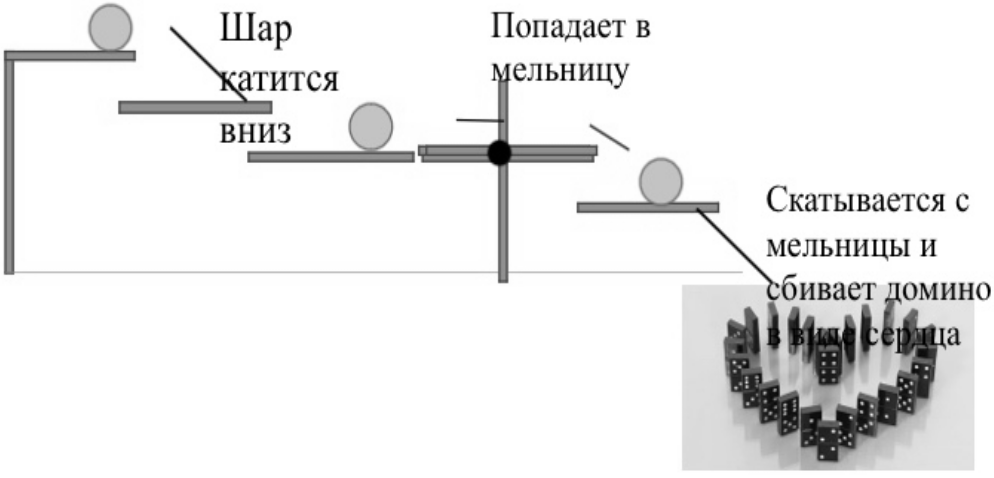
\includegraphics[width=0.7\textwidth]{authors/leybovich-fig2.png}
  \end{center}
  \caption{Схема установки <<Принцип домино>>}
  \label{fig:leybovich-fig2}
\end{figure}



Третья установка имеет более сложную комплектацию и включает множество различных деталей~--- детскую машинку, дорожку для её движения, пластиковые фишки домино, маленькие железные шарики, качели-балансиры, пластиковую трубу и маятник (рис.3). Её назначение также заключается в демонстрации законов сохранения и импульса. Для её построения на стул устанавливается небольшая горка. Из семи деревянных дощечек (которые вырезаются из одной большой доски), строятся дорожки. На одной из них, расположенной горизонтально, ставятся фишки домино. В конце дорожки размещается шарик. Другая дощечка располагается под углом (чтобы шарик смог скатиться). Качели-балансиры изготавливаются самостоятельно из простой дощечки и любой опоры. Для установки трубы также используется любая опора (можно выбрать небольшую коробочку или маленький стульчик). По желанию маятник тоже можно изготовить самостоятельно, но его не сложно приобрести и в магазинах.

\begin{figure}[h!]
  \begin{center}
    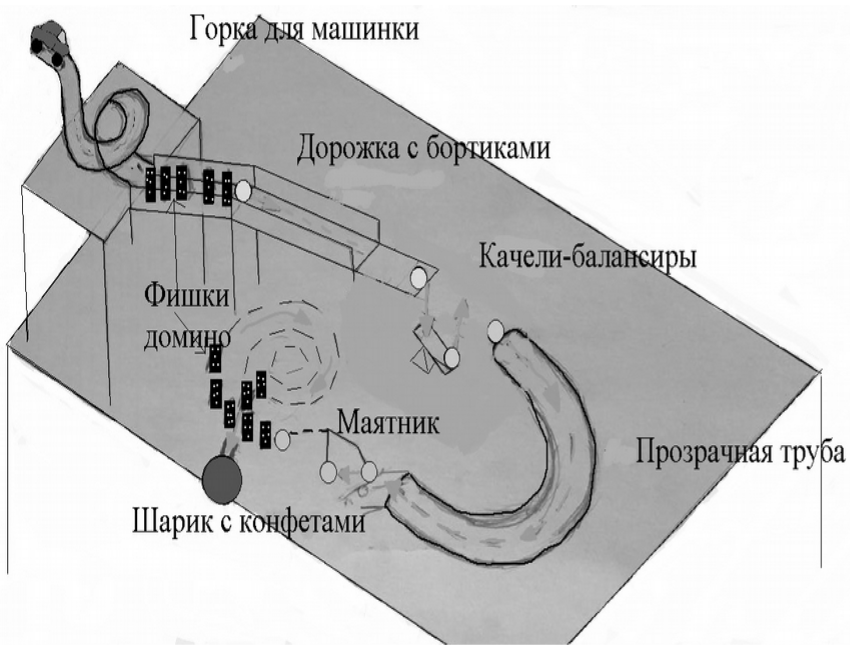
\includegraphics[width=0.9\textwidth]{authors/leybovich-fig3.png}
  \end{center}
  \caption{Схема установки <<Конвейер>>}
  \label{fig:leybovich-fig3}
\end{figure}


Вся работа данной конструкции заключается в том, что предметы, передавая друг другу импульс и энергию, вызывают цепную реакцию движения. На небольшой высоте над поверхностью закрепляется направляющая дорожка, по которой запускается машинка. Скатившись, и набрав скорость, она толкает фишки домино, которые в свою очередь, приводят в движение шарик.  Шарик падает на качели-балансиры, что позволяет другому шарику подняться под углом вверх и попасть в пластиковую трубу. На выходе из трубы, шарик толкает дощечку, удерживающую на небольшой высоте маятник. Вследствие этого маятник начинает колебаться и толкает фишки домино, которые рушатся и складываются в красивый рисунок. Бонус - последняя фишка домино толкает в руки детям шарик с конфетами внутри.

В заключение отметим, что общение разных поколений в ходе конструирования представленных установок, позволяет обмениваться им своими знаниями и умениями. А для поколения Z, вступающего в ближайшем будущем в активную профессиональную жизнь, такие занятия позволяют более осознанно принимать решения о выборе своей инженерной специальности. Разработанные нами установки позволяют тренировать и развивать интерес и способности к конструированию и проектированию, что впоследствии сыграет важную роль в освоении новых профессий будущего.

\begin{thebibliography}{99}
\bibitem{}\BibAuthor{}Какие профессии будут востребованы через 5--7 лет [Электронный ресурс].~--- URL: https://www.iqconsultancy.ru/articles/kakie-professii-budut-vostrebovany-cherez-5-7-let/ (дата обращения 25.03.2020).

\bibitem{}\BibAuthor{}5 особенностей поколений Z, которые стоит учитывать, чтобы найти с ними общий язык [Электронный ресурс].~--- URL: https://lifehacker.ru/mif-pokolenie-z/ (дата обращения 5.04.2020).
\end{thebibliography}


\rasdelL{Вопросы истории \\[04pt]
 и~социально-экономического развития северных
 территорий}{Вопросы истории и~социально-экономического развития северных
 территорий}
\procTitle{Социокультурный и этноисторический контекст развития Магаданской области (на примере эвенов)}
\procAuthor{Егян~А.\,А.}
\procEmail{Artemio01091939@gmail.com}
\procOrganization{СПбГУ} \procCity{Санкт-Петербург}

\makeProcTitleRazdel
\index{e@Егян~А.\,А.}


Коренным населением Магаданской области являются эвены, народ тунгусо-маньчжурского происхождения, связанный историко-культурными и хозяйственными связями с соседними народами: якутами, коряками, юкагирами, чукчами, эвенками и так далее. Однако на территории Магаданской области эвены в количественном измерении абсолютно доминируют во всех районах над другими коренными малочисленными народами Севера (КМНС) РФ.

     Социокультурные связи эвенов неразрывным образом связаны с древностями, эпохой колонизации и новейшей историей Магаданской области, в большинстве контекстов отображая историю её освоения и развития.

     Этноисторический контекст эвенов является близкой по ряду факторов к другим народами Северо-Востока России, особенно коряков, эвенков, частично юкагирам и в меньшей степени якутам. Этническая и историческая форма восприятия эвенов сквозь призму вклада в генезис культуры Магаданской области, которая является отличительной чертой данного субъекта на фоне соседей, имеющих другой бэкграунд, позволяет раскрыть культурно-антропологический пласт бассейна Колымы.

      Контекст современной экологии и аспектов её влияния на этносоциальный контекст эвенской жизни неоднозначен. Историческая деятельность колымских разработок, особенно золотоносных, связанная также и с деятельностью Дальстроя, повлияла на физико-географические свойства локальной природы, например, на рыбохозяйственную сторону деятельности, ибо в бассейне Колымы (верхней) пришел в упадок естественный прирост и развитие рыбы, что в суммарном эквиваленте бассейного измерения превышает 150~рек [1].

      Проблемы касаются и с площадью потерянных для хозяйственного контекста (нарушенного) для оленеводства (оленьих пастбищ), характерного эвенам исторически.

      Волны проблем коснулись и группы эвен Северо-Эвенского района Магаданской области (Кубакинское, Пеледонское), которые столкнулись с золоторудной добычей и сложностей с привычным использованием в традиционной нише для оленеводства.

      Районы, находящиеся в непосредственной близости от трассы в Якутию, также испытывают влияние на традиционный быт эвенов данного региона: как Магаданской области, так и собственно Якутии (Усть-Янский улус; Булунский, Аллайховский в контексте деградации пастбищ). В то же время Момский улус, где расположены эвенские исторические поселения, считается заповедной; в ней технологические разработки запрещены и ограничены [2].

      Традиционным контекстом деятельностью эвенов, связанный с древностью Магаданской области, является оленеводство (кочевого происхождения), а также охота на белку. Эвены Охотского моря также связаны с ловлей рыбы и морского зверя. Между эвенами происходил обмен товарами натурального хозяйства (например, мясо оленей на шкуру нерпы).

      В XX веке, в эпоху коллективизации, стада оленей обобществились, крупнейшие стада включали в себя более двадцати пяти тысяч оленей в эвенских хозяйствах, которые отличались традиционно высокой продуктивностью. В эпоху 1990-хх гг., связанной с трансформацией экономического направления, появились формы общин (родовых, также семейных), которые получили определённую территорию традиционного пользования (этноисторически). Опыт реорганизации совхозов и близких к ним форм промысловых объединений показывает, что традиционное эвенское хозяйство нуждается в коллективной форме, а также в государственной поддержки [3].

      Эвены относятся к коренному населению Магаданской области и частично соседних субъектов РФ (Хабаровский край, Якутию, Чукотский АО и Камчатская области). Прежде в русском языке существовало название <<ламуты>> (от эвенкийского названия моря).

      Эвенский язык генетически восходит к тунгусо-маньчжурской ветви алтайской семьи языков. В эвенском языке существуют диалекты и говоры, более двух десятков, связанных с географией: восточный, западный и средний. Диалект эвенов Магаданской области является литературной нормой, а письменность в начале 1930-х гг. была на латинице, которая через к середине декады сменилась кириллицей. Менее половины эвенов владеют эвенским языком, что связано с русификацией и индустриализацией, религиозными и политико-правовым бэкграундом в XVIII--XX веках. Генезис части эвенов, особенно связанных с приграничными районами этноисторической зоной расселения (с юкагирами, чукчами, якутами и другими) [4].

      Проблемой для многих малочисленных народов Севера языковая тематика характерна и для эвенов, но говорить об утрате эвенского языка преждевременно. По оценке специалистов, хорошо владеют родным языком лица старшего и многие представители среднего поколений.

      Языковой вопрос эвенов является одной из проблематичных сторон, равно как и для многих народов, входящих в состав КМНС РФ. Однако полная потеря эвенского языка исключается. Владение эвенского языка, как правило, фиксируется у людей старшего и в меньшей степени среднего поколения.

      Что касается возрастной когорты молодых людей и представителей среднего возраста, на эвенском языке говорит от менее половины населения, приблизительно 1/5 всех людей, не достигших 18~лет [5].

      Преподавание эвенского языка ограничивается четвёртым классом, в части школ он является факультативным. Использование языка ограничено преимущественно семьёй (реже производством) в случае абсолютного эвенского этнически большинства. Эвенский преподаётся в Магаданском Международном Педагогическом Университете, а также в Хабаровске (Педагогический Университет) и Санкт-Петербурге (РГПУ им. Герцена). Существуют случаи проблемных контекстов (сокращения из-за проблем финансирования): Быстринский район Камчатки, где издаётся газета <<Айдит>>. Художественные направления на эвенском языке издаются Магаданским книжным издательством.

      Эвены являются одним из самых крупных народов, включённых в КМНС РФ. Сложности в реализации традиционных контекстов хозяйства по ряду исторических и других причин, а также социально-экономические трудности в Магаданской области, выраженные в демографических показателях, тем не менее, не препятствуют этносоциальному развитию в дальнейшей перспективе. Разрешение демографических, этнолингвистических, социокультурных и финансовых сторон способствует в будущем развитию социокультурного и этноисторического начала [1].

     Контекст статуса заключается в том, что в Северо-Эвенском районе Магаданском области, равно как и в Быстринском районе Камчатки, де-факто существует институт национального района, что также характерно и для других.

      Органы местного самоуправления взаимодействуют с органами власти и коммерческими структурами (например, по контестам рыбного хозяйства, трудоустройства эвенов). Ассоциация эвенов в Ольском районе распределяет среди эвенов лимиты на улов лосося. В вопросе золоторудных компаний, например, Ассоциация выступает соучредителем, что увеличивает финансовое наполнение и позволяет расходовать деньги по статьям нужд оленеводов, культурной жизни, подготовки специалистов и так далее.

      На эвенов распространяются общие контексты юриспруденции КМНС РФ. В 1998~г. в Магаданской области реализовано положение (временное) <<О~территориях традиционного природопользования малочисленных народов Севера>>, тогда как в соседних субъектах РФ были реализованы иные законы, связанные, помимо эвенов, ещё и с другими народами, преимущественно с относительным большинством из числа народов Северо-Востока:  в Якутии это <<О~территориях традиционного природопользования малочисленных народов Севера>>; в Камчатской области это закон <<О~территориально-хозяйственных общностях КМНС>> и <<О ТТП (1998)>> ; в Чукотском АО это положения (временные) <<О порядке передачи земельных участков под фермерские оленеводческие хозяйства>> [6].

      Что касается этносоциальных контекстов, традиционно выделяемыми проблемами эвенов, прежде всего социального кластера, это безработица и здоровья, особенно что связано с наследием экономических реформ и социально-экономических преобразований, выраженных в показателях безработицы и здоровья. Однако этот контекст связан также и с возвращением части эвенов на родовые места в данный период, форма возврата к натуральному хозяйству (охота, рыболовство, сбор растений) в силу финансовых трудностей.

      Что касается заболеваний, связанных со здоровьем у эвенов Магаданской области, отличаются следующие: проблемы с органами дыхания, сердцем, алкоголизмом и связанные с ним отравления, туберкулёзом [7].

      В XVII веке эвены имели географическое распространение по отрогам Верхоянского хребта, по Колыме и притокам, омолонским и индигирским бассейнам. Так, сужение привычного ареала хозяйственного и другие причины, вытекающих из колонизации со стороны Юго-Запада, привели к миграции также и в зону Уды и Амгуни.

      В Магаданской области (наиболее эвенскими) по этническому составу районами проживания являются следующие: Ольский и Северо-Эвенский. Историческими событиями для эвенов является так называемое <<восстановление национальности>>, прежде всего в Якутии и в меньшей степени в Хабаровском крае.

      Таким образом, в данной статье раскрываются социокультурный аспект формирования и развития эвенов в общем дискурсе Магаданской области на материалах этнической и социальной истории, а также хозяйственных, правовых, культурологических, социально-экономических аспектов.

     Эвены являются одним из крупнейших народов по численности, включённых в состав КМНС РФ. Однако контексты массового притока русскоязычного населения в 20 веке (различного по этническому и культурно-социальному происхождению), активное вовлечение в образование в русском среде, промышленного освоения, деятельности Дальстроя и др., сформировали особенную социокультурную и этнолингвистическую ситуацию, уникальную для Северо-Востока России.

      Значительная вовлеченность в процессы XX~века, особенно связанной с притоком населения, оторванного от прежней среды, принципиально различной по происхождению, а также связь с древними культурно-антропологическими пластами бассейна Колымы, повлияли на формирование современных контекстов в жизни эвенов Магаданской области.


\begin{thebibliography}{99}

\bibitem{}\BibAuthor{Бацаев~И.~Д.}  Очерки истории Магаданской области (начало 20-х~--- середина 60-х~гг. XX~в.).~--- Магадан~: СВКНИИ ДВО РАН, 2007.~--- 17~с.
\bibitem{}\BibAuthor{Козлов~А.~Г.} Магадан: возникновение, становление и развитие административного центра Дальстроя (1929--1945).~--- Магадан~: СВНЦ ДВО РАН, 2007.~--- 126~с.
\bibitem{}\BibAuthor{Левин~М.~Г.} Эвены // Этнографические очерки. Народы Сибири / Под. ред. М.~Г.~Левина и Л.~П.~Потапова.~--- Москва, 1956.~--- С.~26.
\bibitem{}\BibAuthor{Попова~У.~Г.} Эвены Магаданской области. Очерки истории, хозяйства и культуры эвенов Охотского побережья, 1917--1977.~--- М.~: Наука, 1981~--- 304~с.
\bibitem{}\BibAuthor{Сирина~А.~А.} Эвены // Большая российская энциклопедия.~--- Москва, 2017.~--- 204~с.
\bibitem{}\BibAuthor{Суляндзига~Р.~В., Кудряшова~Д.~А., Суляндзига~П.~В.} Коренные малочисленные народы Севера, Сибири и Дальнего Востока Российской Федерации. Обзор современного положения.~--- Москва, 2003.~--- С.~15.
\bibitem{}\BibAuthor{Туголуков~В.~А.} Тунгусы (эвенки и эвены) Средней и Западной Сибири.~--- Москва, 1985.~--- С.~26.

\end{thebibliography}

\procTitle{Опыт определения  предмета охраны археологической стоянки <<поселение Бугурчан II--I~тыс.~до~н.~э. (четыре~жилища)>>}
\procAuthor{Зеленская~А.\,Ю.}
\procEmail{zelenskaya@neisri.ru}
\procOrganization{СВКНИИ ДВО РАН} \procCity{Магадан}

\makeProcTitle
\index{z@Зеленская~А.\,Ю.}

Для постановки на учёт и охрану объектов культурного наследия (в~т.~ч. объектов археологического наследия) в органах исполнительной власти регионов, помимо проведения полевых и камеральных работ, необходимо определить, изучить и описать предмет его охраны. \textbf{Предмет охраны}~--- это особенности объекта культурного наследия, которые представляют его культурную ценность и служат основанием для постановки этого объекта на~государственный учёт.

С правовой точки зрения, необходимость определения предмета охраны, закреплена в Федеральном законе от 25 июня 2002~года 73-ФЗ <<Об объектах культурного наследия (памятниках истории и культуры) народов Российской Федерации>> (статья 15). Изданием приказов об утверждении предметов охраны объектов культурного наследия (далее~--- ОКН) Магаданской области занимается отдел по охране ОКН при Правительстве Магаданской области.

До недавнего времени Отдел по охране ОКН издавал приказы об утверждении предметов охраны только для памятников архитектуры. Определение предмета охраны таких объектов является процессом, зачастую, однозначным и объективным. Например, предметом охраны любого исторического здания, является его конструкция и внутренне убранство (элементы интерьера/экстерьера архитектурного сооружения). Но определение предмета охраны объекта археологического наследия (далее~--- ОАН) сопряжено с рядом трудностей, а именно: 1)~необходимостью актуального мониторинга состояния ОАН и 2)~точным определением границ распространения культурного слоя (который является одним из главных элементов предмета охраны), из чего сразу возникает парадокс~--- изучая культурный слой, мы его одновременно и уничтожаем.

 По заданию отдела по охране ОКН Правительства Магаданской области в~2019~г., сотрудниками лаборатории истории и экономики СВКНИИ ДВО РАН~--- ведущим научным сотрудником, к.\,и.\,н. Слободиным~С.~Б. и младшими научным сотрудником Зеленской~А.~Ю. были выполнены работы по~определению предмета охраны для стоянки-поселения Бугурчан (стоянка находится на~Государственной охране решением исполнительного комитета Магаданского облсовета народных депутатов от 29.04.1974 №~174).

Ранее, в~2017~г., этими же сотрудниками был проведён мониторинг данной стоянки [2], в~результате которого был составлен топографический план, определены границы ОАН посредством заложения шурфов и зачисток, а также локализованы на местности ландшафтные элементы стоянки (местонахождения полууглубленных жилищ).

В процессе работы над проектом был выполнен анализ всей имеющейся учётной документации, публикаций об объекте археологического наследия, выполнен сбор и анализ результатов археологических обследований на~территории расположения объекта археологического наследия (материалы архивного фонда Магаданского областного краеведческого музея и научно-отраслевого архива Института археологии РАН) и результатов археологических работ 2017~г.

Стоянка-поселение Бугурчан находится на полуострове Кони, на южном берегу залива Одян. Она располагается на высокой морской террасе, протянувшейся по~левому берегу р.~Богурчан на территории бывшего пос.~Бугурчан.

Первые сведения о стоянке поступили в Магаданский областной краеведческий музей (далее~--- МОКМ) в~1939~г. от эвена-охотника И.~Бабцева, который сообщал о <<коряцких ямах>> в~устье р.~Богурчан [3]. В~1955~г. археологический отряд Якутского филиала АН СССР и МОКМ (рук. Г.~А.~Пытляков и А.~В.~Беляева) провёл обследование стоянки, представленной тогда выраженными в рельефе западинами округлых в пла­не полуподземных жилищ [4; 5]. В ходе обследования было обнаружено шесть округлых в плане полуподземных жилищ [4, Л.~54]. Одно располагалось у моря, на первой надпойменной террасе р.~Богурчан, вблизи пирса и рыбзавода и было полностью уничтожено морским прибоем, еще 5 жилищ найдено на террасе, где располагался поселок [2, С.~7; 1, С.~144]. Материалы раскопок опубликованы Р.~С.~Васильевским [1, С.~66-69].

При проведении мониторинга в 2017~г. локализовать на местности указанные Г.~А.~Пытляковым жилища не удалось по причине того, что жилища №~1--4, были, очевидно, разрушены при строительстве посёлка и нивелированы с поверхностью террасы хозяйственной деятельностью. Но культурный слой, как выяснилось, сохранился. Судя по разрушенным остаткам пирса и рыбозавода заливаемых морем, и по сообщению живущих там сторожил, морская терраса, где расположена стоянка, была разрушена морем примерно на 10--15~м, так, что жилища №~5 и 6 к настоящему времени полностью смыты морем.
Заложенные по краю террасы и в ее глубине в ходе мониторинга 2017~г. 6 зачисток и шурфов подтвердили наличие на террасе сохранившегося от древнего поселения культурного слоя с находками каменных, костяных орудий и керамики.

Суммируя полученные данные было определено, что мощность культурного слоя стоянки варьируется от 10 до 40 см. Сохранность культурного слоя стоянки средняя, что связано с современной антропогенной деятельностью. Площадь распространения культурного слоя прослеживается от зачистки у берегового обрыва вглубь по террасе на юг на расстояние до 120--130~м. Археологические находки характерны для древнекорякской культуры I--II~тыс.~н.~э.

В соответствии с контекстом изученного археологического материала был описан предмет охраны поселения. Данный археологический объект обладает историко-культурной ценностью, являясь источником информации развитии культуры населения Охотского побережья в позднем голоцене, в~эпоху палеометалла. Стоянка представляет научный интерес в перспективе построения культурно-хронологической схемы развития культур с приморской адаптацией, характеристике культурной принадлежности древних обитателей, техники каменного производства и хозяйственной деятельности. Памятник перспективен для дальнейшего научного изучения. Сохранению подлежат культурные остатки, залегающие на глубине до 0,4~м. Площадь территории объекта и, соответственно, распространения отложений с~культурным слоем, уточнена в результате геодезических работ и составляет 18\,891~м$^2$.

Таким образом, предметом охраны объекта культурного (археологического) наследия федерального значения <<Поселение Бугурчан II--I~тыс. до~н.~э.>> были определены следующие элементы:

1. Территория ОАН в пределах утверждённых границ на общей площади  18\,891~м$^2$ (см.~рис.).

\begin{figure}[h!]
  \begin{center}
    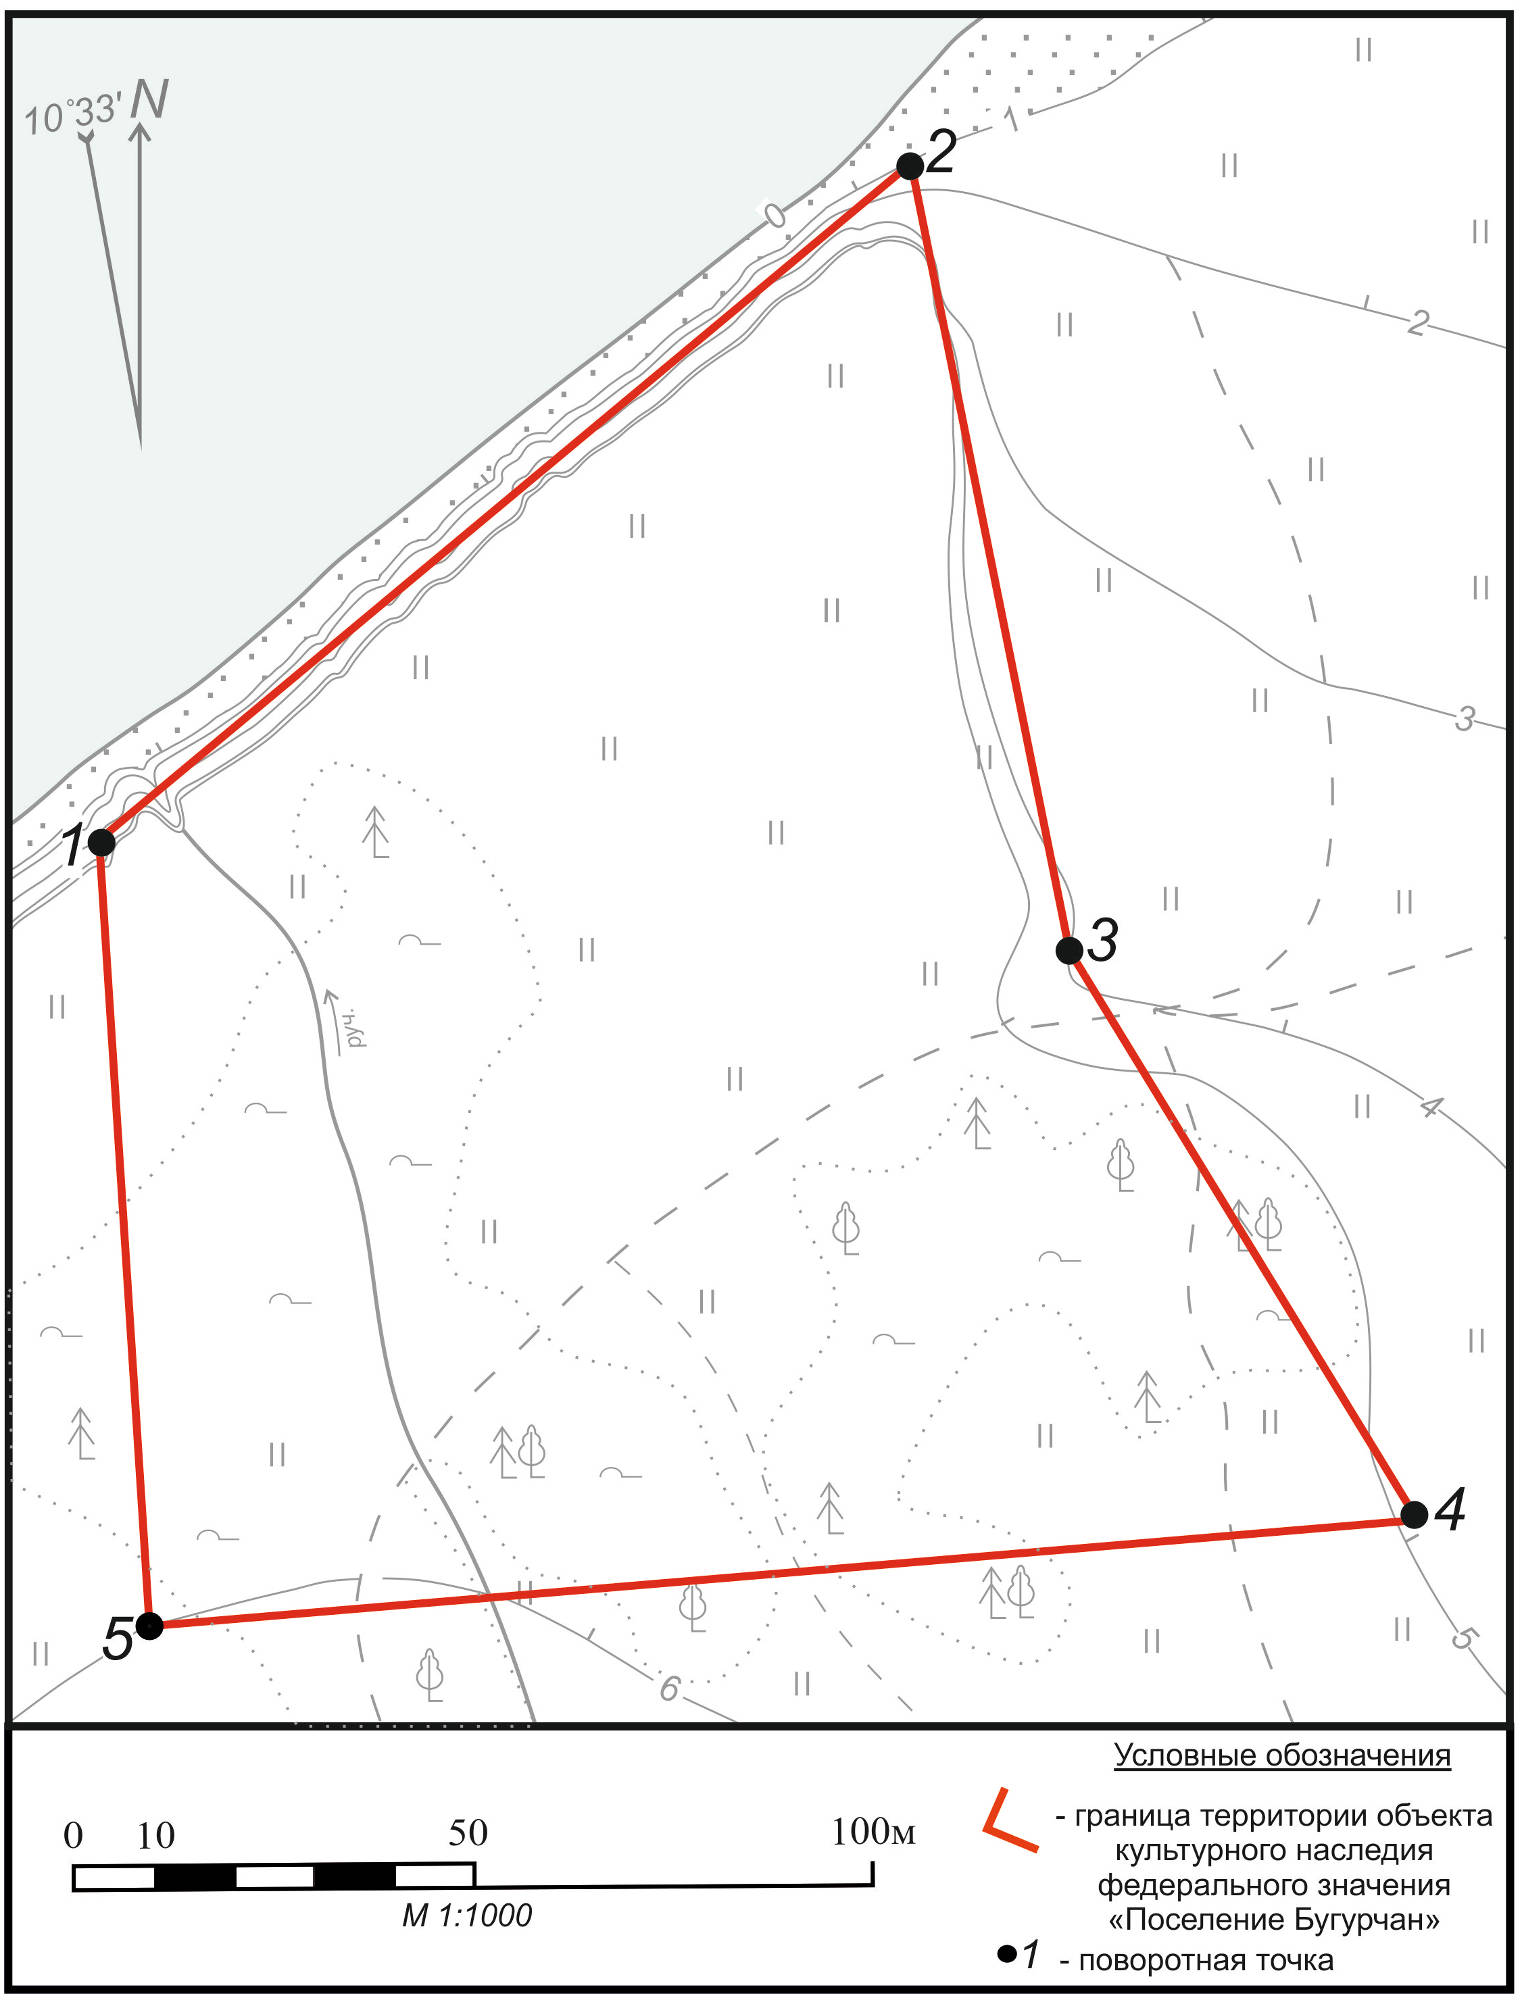
\includegraphics[width=0.8\textwidth]{authors/zelenskay.jpg}
  \end{center}
  \caption*{\textbf{Схема расположения границы территории ОКН <<Поселение Бугурчан>>}}
  \label{fig:zelenskay}
\end{figure}


2. Культурный слой, несущий в себе остатки жизнедеятельности древнего человека, частично или полностью скрытый под землёй (представлен основанием тёмно-коричневой гумусированной супеси в сочетании с кровлей рыжего суглинка или бурой супеси с линзами углистости на глубине от 10 до 40~см от~дневной поверхности.

3. Археологические недвижимые и движимые объекты, содержащиеся на современной дневной поверхности ОАН, в составе грунтовых напластований (конструкции и сооружения, антропологические и остеологические материалы, археологические предметы, следы жизнедеятельности древнего человека): миниатюрное тесло или нож треугольной формы из кремнистой породы; наконечник стрелы треугольной формы из кремнистого сланца с прямыми длинными сто­ронами и небольшой овальной выемкой в основании; массивный наконечник копья или китового гарпуна из тёмного кварцита листовидной формы с черешковым насадом; два продолговатых тесла из чёрного кремнистого сланца с острым обушком, выпуклым широким рабочим краем; два скребка; три грузила для сетей; шесть небольших аморфных нуклеусов а также фрагменты керамики с ложнотекстильным оттиском (материалы раскопок 1956~г.). Отщепы, каменное тесло, костяное орудие и керамика с налепными валиками, отогнутым венчиком, и вафельным отпечатком (материалы мониторинга 2017~г.).

Материалы раскопок стоянки-поселения Бугурчан хранятся в Магаданском областном краеведческом музее и Музее естественной истории СВКНИИ ДВО РАН.

4. Видимые на поверхности сооружения в виде котлованов жилищ и~объектов хозяйственного назначения. В 1955~г. археологический отряд Магаданского краеведческого музея под руководством Пытлякова~Г.~А., в ходе археологической разведки в устье р.~Богурчан, выявил шесть округлых полуподземных жилищ, выраженных в рельефе западинами. В 1956~г. была осуществлена полная раскопка жилища №~1.

В ходе мониторинга 2017~г. выяснилось, что жилища № 5 и 6, которые располагались на краю береговой террасы, были уничтожены морским прибоем. Локализовать на местности указанные Г.~А.~Пытляковым жилища удалось лишь приблизительно по архивным данным, т.~к. видимые западины в рельефе были нивелированы в ходе хозяйственной деятельности по~террасе. Вместе с тем, заложенные на стоянке-поселении стратиграфические разрезы показали наличие сохранившегося культурного слоя, не затронутого в процессе снятия верхнего почвенного горизонта. Таким образом, предметом охраны в данном случае, выступают снивелированные западины жилищ №~1--4.

5. Ландшафтно-пространственное и видовое восприятие участка в границах территории ОАН. В связи  с тем, что объект культурного наследия поселение Бугурчан расположен за пределами градостроительной среды, его ландшафтно-пространственное восприятие строиться на основе анализа физико-географической обстановки. Композиция стоянки, расположенной в природной среде, подчинена её своеобразию.

Стоянка-поселение Бугурчан находится на пол-ве Кони, в~зал.~Одян, на~его южном берегу, на 2-й надпойменной террасе слева от устья р.~Богурчан, где ранее располагался посёлок Бугурчан. На левом берегу р.~Богурчан выделяются первая и вторая надпойменные террасы. Первая надпойменная терраса имеет чётко выраженный тыловой шов на стыке со второй надпойменной террасой, на которой и расположена стоянка Бугурчан. В районе берега моря сочленение террас образует своеобразную <<стрелку>>, с которой открывается хороший обзор как в обе стороны по берегу моря, так и~вверх по долине р.~Богурчан. B 400--450~м от её устья, в долине р.~Богурчан происходит нивелировка первой и второй террас в одну.

Высокая, пологая, с небольшим подъемом вторая надпойменная терраса на левом берегу р.~Богурчан протянулась от ее устья к западу, вдоль берега моря и к югу, по долине р.~Богурчан на несколько сотен метров. Тыловой шов визуально не выделяется. Береговой уступ террасы со стороны моря обращён к северу (имеет северную экспозицию), обрывист, но хорошо задернован, высотой до 5~м. Подвергается разрушению только в сильные шторма. В~120~м от её края (от <<стрелки>>) в море впадает небольшой ручей, который, видимо, служил источником питьевой воды для древнего населения, обитавшего на этой террасе. По левому берегу ручья отмечены заболоченные участки террасы.

Вторая надпойменная терраса, на которой локализована стоянка Бугурчан, представляет собой открытую пространственную единицу ландшафта. Конфигурация зрительных барьеров сложена из низкорослого древостоя террасы, локализованного в её обрамлении (с восточной и южной стороны) и хозяйственных построек. Существующие постройки ввиду своих малых габаритов (не более 8~м в~высоту) и разреженности, не препятствуют визуальному изучению участка расположения ОКН. Таким образом, обзор на~стоянку не имеет ограничений.

Наиболее оптимальной зоной восприятия памятника является приустьевая часть террасы р.~Богурчан, точка обзора~--- в направлении восток-запад, и подножие сопки на юго-востоке, точка обзора~--- в направлении юго-запад~--- северо-восток. Таким образом, предметом охраны выступает обеспечение визуального восприятия объекта культурного наследия в его исторической и природной среде (запрещение перекрытия основных видовых точек и панорам, нарушающих визуальное восприятие объекта культурного наследия в его исторической среде).

Подводя итог проделанной работе по определению предмета охраны ОАН стоянки-поселения Бугурчан, необходимо отметить важность предварительно проведённых полевых работ, которые позволили определить утерянные для охраны элементы стоянки (разрушенные морским прибоем, жилища №~5 и 6), а также произвести поиск сохранившегося культурного слоя. Таким образом, все элементы и качественные особенности археологической стоянки, зафиксированные при проведении мониторинга в 2017~г., были поставлены на охрану Приказом Отдела по охране объектов культурного наследия Правительства Магаданской области №~23 от 11.12.2019.

\begin{thebibliography}{99}

\bibitem{}\BibAuthor{Васильевский~Р.~С.} Происхождение и древняя культура коряков.~--- Новосибирск, 1971.~--- 252~с.

\bibitem{}\BibAuthor{Пытляков~Г.~А., Беляева~А.~В.} Археологические работы на Охотском побережье //  Краеведческие записки.~--- Магадан~:МОКМ, 1957.~--- Вып.~I.~--- С.~5--11.

\textbf{Архивые источники}

\bibitem{}\BibAuthor{Зеленская~А.~Ю.} Научный отчёт по теме <<Археологические исследования в~Омсукчанском, Тенькинском, Ольском, Хасынском городских округах и~в~муниципальном образовании ,,\,г.~Магадан\,‘‘ Магаданской области в 2017~г. В~2-х~томах>> // Научно-отраслевой архив ИА~РАН. Ф.~1.
\bibitem{}\BibAuthor{Пытляков~Г.~А.} Отчёт и материалы предварительного исследования археологических памятников разведывательным отрядом Якутского филиала АН~СССР и Магаданского музея // МОКМ. Оп.~1. Д.~235.
\bibitem{}\BibAuthor{Пытляков~Г.~А.} Отчёт о проделанной работе археологическим разведывательным отрядом в верховьях реки Индигирки и на побережье Охотского моря летом 1955 г. // Архив ИА РАН. Ф.~1. Р.~1. №~1100. 94 л.



\end{thebibliography}


\procTitle{Техносферные пожары: социально-экономические последствия
(на примере Магаданской области)}
\procTitleNewLine{Техносферные пожары: социально-экономические последствия\\(на примере Магаданской области)}

\procAuthorI{Зеленцов~Н.\,С.}
\procEmailI{zelentsovnikita@mail.ru}
\procOrganizationI{ФГБУ СЭУ ФПС ИПЛ}
\procCityI{Магадан}

\procAuthorII{Лунегова~А.\,А., Болотин~А.\,В.}
\procEmailII{laaru@rambler.ru, alexandr\_bolotin@mail.ru}
\procOrganizationII{СВГУ}
\procCityII{Магадан}

\makeProcTitleIINewLine
\index{l@Лунегова~А.\,А.}
\index{b@Болотин~А.\,В.}
\index{z@Зеленцов~Н.\,С.}

Вопросы защищённости личности, имущества, общества и государства от пожаров являются приоритетными [4]. Возникновение пожаров и их последствия наносят огромный вред экономике страны. Пожары нарушают жизнь работников, работодателей и их семей. В~целях минимизации жертв и ущерба важно знать показатели возможной пожарной опасности объекта, её последствий для людей и имущества, то есть пожарный риск. Именно поэтому ситуация с пожарами требует дополнительного изучения, так как показатели по их количеству и последствиям заметно превышают количество и последствия происшествий иного характера.

Федеральным законом № 123-ФЗ установлено нормативное значение индивидуального пожарного риска (R$_H$), равное 10$^{-6}$ (1/чел.$\cdot$год) [3]. Для оценки пожарных рисков территорий (субъектов, городов, сельских поселений и др.) под руководством Н.~Н.~Брушлинского разработан ряд отдельных (частных) пожарных рисков [1], которые ориентированы на оценку социального и экономического ущерба (по отдельности друг от друга).

Социальные риски сопряжены с опасностью для людей. Для их оценки применены следующие показатели:
\begin{enumerate}[noitemsep]\vspace{-8pt}
  \item показатель R$_1$ подразумевает возможность человека столкнуться с~пожаром при~проживании или пользовании объектом и инфраструктурой:\\
  $$R_{1}=\frac{P}{N}\left(\dfrac{\text{пожар}}{\text{чел.}}\right),$$\\
  где Р~--- количество пожаров в год, ед.; N~--- количество людей, столкнувшихся с~пожаром при~проживании или пользовании объектом и~инфраструктурой, чел.;
  \item показатель R$_2$ подразумевает, что человек может пострадать при пожаре и сопутствующих обстоятельствах:\\
  $$R_{2}=\frac{N_\text{Ж}}{P}\left(\dfrac{\text{жертва}}{\text{пожаров}}\right),$$\\
  где N$_\text{Ж}$~--- количество жертв пожара, чел.; Р~--- количество пожаров в~год, ед.;
  \item показатель R$_3$ характеризует опасность погибнуть при возгорании:\\
    $$R_{3}=\frac{N_\text{Ж}}{T}\left(\dfrac{\text{жертва}}{\text{год}}\right),$$\\
    где N$_\text{Ж}$~--- количество жертв пожара, чел.; T~--- промежуток времени, год.
\end{enumerate}
 \vspace{-8pt}
\clearpage
К экономическим рискам относятся риски, сопряжённые с потерей материальных ценностей. Для их оценки применены следующие показатели:
\begin{enumerate}[noitemsep]\vspace{-8pt}
  \item показатель R$_4$ характеризует риск уничтожения строений в результате пожара:\\
  $$R_{4}=\frac{N_\text{стр.}}{P}\left(\dfrac{\text{уничт. стр.}}{\text{пожар}}\right),$$\\
  где N$_\text{стр.}$~---  количество уничтоженных строений в результате пожара, ед.; Р~--- количество пожаров в~год, ед.;
  \item показатель R$_5$ характеризует риск прямого материального ущерба:\\
  $$R_{5}=\frac{D}{P}\left(\dfrac{\text{ден. ед.}}{\text{пожар}}\right),$$\\
    где D~--- сумма ущерба, руб.; Р~--- количество пожаров в~год, ед.
\end{enumerate}
 \vspace{-8pt}

 Разберём расчёт социальных и экономических последствий пожаров на~материалах Управления надзорной деятельности и профилактической работы Главного Управления МЧС России по Магаданской области [2]. На~рис. 1 представлены данные о пожарах, жертвах и ущербе по Магаданской области.

\begin{figure}[H]
%\begin{changemargin}{-1cm}{0cm}
  \begin{center}
    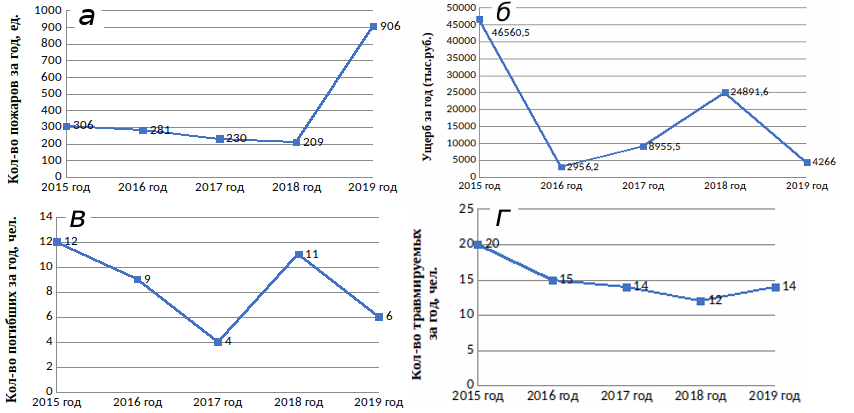
\includegraphics[width=1\textwidth]{authors/zelencov_fig1.png}
  \end{center}
%  \end{changemargin}
  \caption{Количество пожаров (\textit{а}); ущерб, причиненный пожарами (\textit{б}); количество погибших (\textit{в}) и~травмированных (\textit{г}) за 2015--2019 гг.}
  \label{fig:zelencov-fig1}
\end{figure}


Исходя из рис. 1,\textit{а}, можно сделать вывод, что за 2019\,г. увеличился рост пожаров в Магаданской области (увеличение на 321,4\,\%) в~сравнении с аналогичными периодами.

Объектами возникновения пожаров были:
\begin{enumerate}[noitemsep]\vspace{-8pt}
\item жилой сектор~--- 210 пожаров, что составило 23,2\,\% от общего количества, увеличение на 42,9\,\%;
\item места открытого хранения веществ и материалов и прочие объекты~--- 578 пожаров (63,8\,\%), увеличение на 100\,\%;
\item транспортные средства~--- 47 пожаров, что составило 5,2\,\% от общего количества; увеличение на 80,8\,\%;
\item здания учебно-воспитательного назначения~--- 1 пожар, что составило 0,1\,\%, увеличение на 100\,\%;
\item здания производственного назначения~--- 26 пожаров, что составило 2,9\,\% от общего количества, увеличение на 85,7\,\%.
\end{enumerate}
 \vspace{-8pt}

 Исходя из рис. 1,\textit{б}, мы видим, что прямой материальный ущерб причинен в~размере 4266,4\,тыс. руб., снижение на 83,0\,\% (20\,830,9\,тыс. руб. за 2018\,г.). Спасено материальных ценностей на сумму 29\,451,3\,тыс. руб.

 Исходя из рис. 1,\textit{в}, можем наблюдать снижение количества погибших людей на 100\,тыс. населения на 45,5\,\% за 2019\,г. При пожарах погибло 6\,чел.

 Причиной гибели людей на пожарах за 2019~г. явилось алкогольное
 опьянение: из шести погибших при пожарах все они находились в~состоянии алкогольного опьянения.

 По социальному статусу среди погибших: 3~пенсионера, 1~рабочий, 2 человека~--- это люди без определённого места жительства.

 По возрастному показателю среди погибших: 1~чел. в~возрасте от~21
 до~40~лет, 4~чел. в~возрасте от~41 до~60~лет, 1~чел. в~возрасте старше 60~лет.

Причинами возникновения пожаров с гибелью людей являются:
\begin{enumerate}[noitemsep]\vspace{-8pt}
\item неосторожное обращение с огнём (при курении)~--- 4 пожара (66,7\,\%), при которых погибло 4 чел. (66,7\,\%);
\item неосторожность при приготовлении пищи~--- 1 пожар (16,7\,\%), при котором погиб 1 чел. (16,7\,\%);
\item нарушение правил эксплуатации электрооборудования~--- 1 пожар (16,7\,\%), при котором погиб 1 чел. (16,7\,\%).
\end{enumerate}
\vspace{-6pt}

Из рис. 1,\textit{г} следует, что за 2019~г. при пожарах травмировано 14~чел. (увеличение на 16,7\,\% + 2~чел.).

Из 14 травмированных при пожаре 10 чел. (71,4~\%) находились в~состоянии
алкогольного опьянения, причём все они были проинструктированы по мерам
пожарной безопасности.

По социальному статусу среди травмированных: 8~чел. без определённого
места жительства (53,8~\%), 2~пенсионера (15,4~\%), 3~рабочих (23,1~\%), 1~индивидуальный предприниматель (7,7~\%).

По возрастному показателю среди травмированных: 4~чел. (27,3~\%) от~21 до~40~лет, 8~чел. (63,7~\%) от~40 до~60~лет, 1~чел. (9,1~\%) старше 60~лет.

Причинами возникновения пожаров с травматизмом людей являются: аварийный режим работы электрооборудования~--- 3~пожара (23,0\,\%), при~которых травмированы 3~чел. (23,0\,\%), неосторожное обращение с огнём, в~том числе при курении,~--- 10~пожаров (69,2\,\%), при~которых травмированы 10~чел. (69,2\,\%), 1~пожар (7,7\,\%) прочие причины, 1~чел. (7,7\,\%) травмирован.

В 2015 г. среди трудоспособного населения во время пожаров получили травмы различной степени тяжести 20~чел., среди них 17~чел. в~г.~Магадане, 2~чел. в~Сусуманском городском округе, 1~чел. в~Тенькинском городском округе, 1~чел. в~Хасынском городском округе.

В 2016 г. среди трудоспособного населения во время пожаров получили травмы различной степени тяжести 15 чел., среди них 12~чел. в~г.~Магадане, 1~чел. в~Ольском городском округе, 1~чел. в~Северо-Эвенском городском округе, 1~чел. в~Сусуманском городском округе.

В 2017 г. среди трудоспособного населения во время пожаров получили травмы различной степени тяжести 14 чел., среди них 12~чел. в~г. Магадане, 1~чел. в~Ольском городском округе, 1~чел. в~Сусуманском городском округе.

В 2018 г. среди трудоспособного населения во время пожаров получили травмы различной степени тяжести 12 чел., среди них 9~чел. в~г. Магадане, 1~чел. в~Сусуманском городском округе, 2~чел. в~Ягоднинском городском округе.

В 2019 г. среди трудоспособного населения во время пожаров, получило травмы различной степени тяжести 14 чел., среди них 13~чел. в~г. Магадане, 1~чел. в~Хасынском городском округе.

На рис.~2 показаны социальные и экономические последствия пожаров.

\begin{figure}[H]
%\begin{changemargin}{-1cm}{0cm}
  \begin{center}
    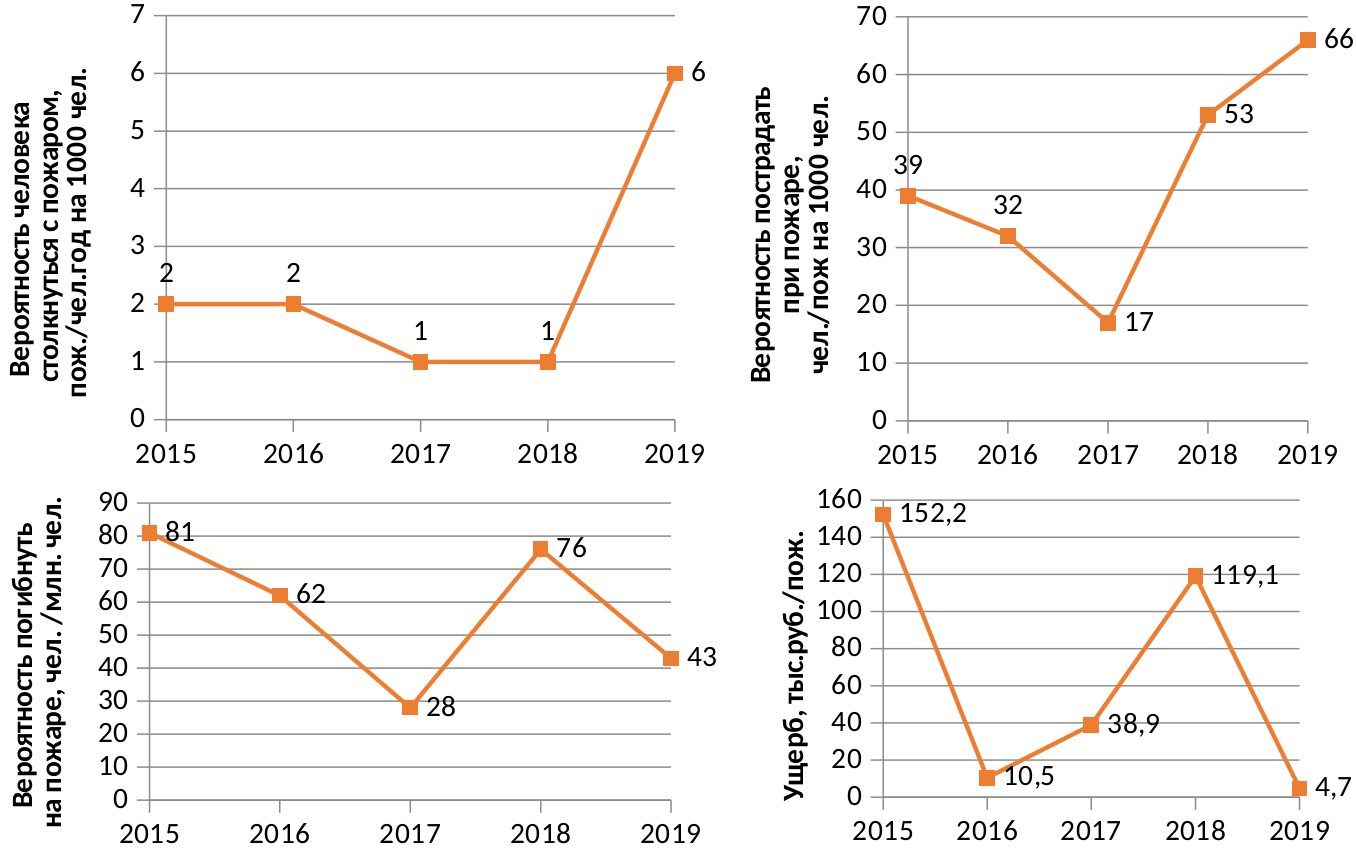
\includegraphics[width=1\textwidth]{authors/zelencov_fig2.png}
  \end{center}
%  \end{changemargin}
  \caption{Социальные и экономические последствия пожаров}
  \label{fig:zelencov-fig2}
\end{figure}


Авторами применён вероятностный подход для вычисления последствий
пожаров.

Социальные последствия пожара характеризуются вероятностью человека
столкнуться с пожаром, вероятностью пострадать на пожаре и вероятностью
погибнуть при пожаре. В~соответствии с теорией вероятности, с пожаром
может столкнуться каждый житель Магаданской области. Ввиду увеличения
количества пожаров в 2019~г. по сравнению с 2015~г. втрое эта
вероятность также увеличилась в 3~раза и составила 6~чел. на 1000~чел.
населения (показатель R$_1$).

Вероятность пострадать при пожаре (показатель R$_2$) по Магаданской
области возросла, что также связано с увеличением количества пожаров.
Вероятность погибнуть при пожаре (показатель R$_3$) находится в~прямой
зависимости от числа жертв (см. рис.~1,\textit{в}), поэтому наблюдается сначала
рост, а~затем спад этого значения.

Несмотря на возросшее количество пожаров в 2019~г. по~сравнению с~2018~г., причинённый материальный ущерб (показатель R$_5$) снизился в~разы, что свидетельствует об эффективности и слаженности работы сотрудников МЧС.

Принимая во внимание причины гибели людей, количество пожаров на объектах гражданского строительства, причины возникновения пожаров, можно дать следующие рекомендации и предложения по профилактике пожаров:
\begin{enumerate}[noitemsep]\vspace{-8pt}
  \item совершенствовать работу по информационному обеспечению и противопожарной пропаганде;
  \item задействовать личный состав пожарных подразделений на проверку жилых домов, обратив особое внимание при обследованиях на состояние электропроводки и печного отопления;
  \item провести профилактические мероприятия с одинокими пенсионерами и инвалидами, неблагополучными семьями;
  \item организовать и проводить мероприятия по обеспечению пожарной безопасности при подготовке жилищного фонда к пожароопасным сезонам;
  \item активизировать проведение комплекса противопожарных мероприятий, направленных на стабилизацию обстановки с пожарами в жилищном фонде Магаданской области;
  \item информировать людей о соблюдении требований пожарной безопасности путём размещения требований пожарной безопасности на квитанциях об оплате жилищно-коммунальных услуг и квитанциях об оплате за услуги в детских дошкольных образовательных учреждениях.
\end{enumerate}
\vspace{-8pt}

\begin{thebibliography}{99}
\bibitem{}Пожарные риски / Н.~Н.~Брушлинский, О.~В.~Иванова, Е.~А.~Клепко, С.~В.~Соколов, С.~Ю.~Попков.~--- М.~: Академия МЧС России, 2016.~--- 66~с.
\bibitem{}Статистические данные ФГБУ СЭУ ФПС ИПЛ по Магаданской области и УНД и ПР ГУ МЧС России по Магаданской области за 2015--2019 гг.
\bibitem{}Федеральный закон Российской Федерации от 22 июля 2008 г. № 123-ФЗ  <<Технический регламент о требованиях пожарной безопасности>>.
\bibitem{}Федеральный закон Российской Федерации от 21.12.1994 г. № 69-ФЗ (ред. от 27.12.2019 г.) <<О~пожарной безопасности>>.
\end{thebibliography}

\procTitle{Стоянка эпохи верхнего палеолита в Волго-Окском междуречье}
\procAuthor{Исмагилова~Е.\,Э.}
\procEmail{yekaterina.ismagilova.97@bk.ru}
\procOrganization{ЕИ КФУ} \procCity{Елабуга}

\makeProcTitle
\index{i@Исмагилова~Е.\,Э.}

% УНИКАЛЬНОСТЬ ТЕКСТА ~45%, много прямых заимствований. см. скриншот.
% Реферативная работа, отстутствует научная составляющая автора.

Палеолит Волго-Окского междуречья является крaйне интересной, но недостаточно исследованной темой. Памятники верхнего палеолита располагаются в различных геолого-геоморфологических условиях: в долинах рек и на междуречьях, в равнинных и горных местностях. Многие из них содержат культурные слои с остатками жилых строений, с многочисленными предметами из кремня, костей млекопитающих и т.\,п [5 С.\,56].

В эпоху палеолита климат Земли, её флора и фауна достаточно сильно отличались от современных климатических условий. Данный этап, межледниковье, характеризовался довольно тёплым климатом, периодически аналогичным современному, отсутствием ледникового покрова в рамках всей Русской равнины. Благоприятные условия выделяются в средневалдайском межледниковье этот этап насчитывает три периода разделённых на более холодные фазы. С 30-го по 22-е тысячелетие, это заключительный период, именно для него был характерен мягкий климат, и он же является самым продолжительным. Начало позднего валдая или осташковское время, 24--20 тыс.\,л.\,н., характеризовалось плавным похолоданием это происходило из-за наступления ледника, который, около 20--18 тыс.\,л.\,н., смог достичь максимального распространения. Этот период является самым холодным в течение всего вюрма. Окончание вюрма, позднеледниковье, 15--13, 5--12 тыс.\,л.\,н.,~--- время, когда климат становится мягче из-за отступления ледника, происходившего не планомерно, а своеобразными пульсациями, то есть период потепления сменялся с периодом похолодания [5 С.\,56]. По мере того как менялся климат, приближался или же наоборот отступал ледник, можно сделать вывод, что древние люди вели полукочевой образ жизни.

В зависимости от изменения климатических условий, группа животных в разных регионах периодически менялась. В период последнего оледенения (20--10 тыс.\,л.\,н.), на территории России оно достигло до верхнего течения Оки и среднего течения Волги, данное оледенение называется окским. В период Окского оледенения некоторые теплолюбивые животные стали вымирать или уходить в более тёплые места, а на смену им, ближе к леднику, пришли такие животные как мускусный бык и северный олень. После на территории Европейской России льды днепровского оледенения, которые разделились на две части, стали доходить до района Днепровских порогов и возможно до района современного Волго-Донского канала. Из-за холодного климата на данную территорию пришли такие животные как: мамонты, шерстистые носороги, дикие лошади, бизоны и т.\,д. Это может быть связано с самым большим похолоданием того периода и обусловленным этим обширным продвижением окололедниковых рельефов [7]. Основная причина исчезновения и снижения популяции различных видов животных заключается в значительном изменении климата и ландшафтов, а не промысловая деятельность человека.

В валдайский этап сплошной массив льда был несравненно меньше по размеру. К нему вплотную примыкала зона своеобразной приледниковой растительности, состоявшей из горно-тундровых, лесных и степных видов. Южнее находилась зона лесостепи, а за ней~--- обширные степные пространства. Это было время наиболее широкого распространения <<мамонтовой фауны>>~--- мамонта, шерстистого носорога, северного оленя, песца, обского лемминга, сайги, байбака [3 С.\,9].

Не только животные и растения <<подстраивались>> под суровые климатические условия, также и древний человек приспосабливался к ним. Они сооружали свои жилища и землянки у водоёмов, в основном у рек, и как только глобальные климатические условия менялись, человек уходил на другое место. Из-за обмельчания, разлива или же перемены прежнего направления реки, эти <<дома>> могли быть уничтожены. В свою очередь не только природные стихии устраняли данную <<преграду>> ещё и животные эмигрируя в другую местность, возможно, уничтожили многие поселения того времени, это и могло являться причиной того, что данные стоянки не все <<дошли>> до нашего времени.

За время раскопок учёные нашли огромное количество находок и отдельных предметов. На обнаруженных стоянках археологи находят изделия из мамонтовой кости, погребения древних людей, много орудий труда, предметов быта, ремёсел, украшений, оружия того времени. Найдены жезлы, дротики и копья из бивней мамонта, кремниевые наконечники, диски из мамонтовой кости с прорезями. Найдены украшения на верхней и нижней одежде, браслеты (под коленями и выше стопы), а также цельные кольца на пальцах. Найдено ожерелье, при изготовлении которого поверхность бусин обработана так, чтобы соседние бусины располагались перпендикулярно друг другу [4 С.\,154; 6].

Редкими произведениями первобытного искусства являются найденные фигурки животных~--- мамонта, лошади-сайги. Так же Зарайский бизон был найден в 2001 г. на дне ямы, примыкающей к очагам жилищно-хозяйственного комплекса стоянки. Его возраст~--- 22--23 тыс.\,л. [1]. И это самое настоящее произведение древнего искусства, работа выполнена на высоком уровне, можно рассмотреть мельчайшие детали, например, глаза, рот, челка и т.\,д. Данная фигурка была сделана из бивня мамонта и использовалась «магических» целях, например, охотники проводили ритуал перед охотой. Примечательно то, что у фигуры бизона отсутствовали два копыта, в шею был помещен кусочек кости, возможно, это могло означать копье или другое оружие того времени, так же с одной стороны он был выкрашен охрой, то есть краской, что могло означать кровь.

Существуют небольшие захоронения мамонтов по всей стране, но самое знаменитое кладбище шерстистых млекопитающих находится на территории Сибири в месте под названием Волчья Грива. При раскопках в 1957 г. впервые были найдены кости мамонта, бизона и лошади, а дальнейшие исследования позволили установить, что 14--11 тыс.\,л.\,н. в этой местности обитали последние сибирские мамонты. В те времена Волчья Грива представляла собой длинный и узкий полуостров среди болот и озер, который заканчивался крутым обрывом. В наши дни~--- это палеонтологический памятник природы областного значения. Уже обнаружено более 600 останков мамонтов. Такой высокой численности остатков доисторических животных ни на Волчьей Гриве, ни в каком-нибудь другом мамонтовом местонахождении России не встречается. Помимо мамонтов, было найдено несколько костей, принадлежавших бизону, лошади, хищникам (вероятно, лисе или песцу) и грызунам.

На данный момент, на территории Волго-Окского междуречья, известны лишь некоторые поселения эпохи Верхнего Палеолита: Сунгирь, Зарайск и т.\,д.

1) Стоянка <<Сунгирь>> открыта в 1955 г. и именно с этого времени начались ее планомерные раскопки. Они велись комплексной экспедицией, возглавляющейся О.\,Н.\,Бадером [4 С.\,201]. Благодаря тому, что смогли найти учёные экспедиции во время раскопок, свыше 50 тыс. отдельных предметов, позволили восстановить жизнь древнего человека приблизительно с исчерпывающей полнотой. Сегодня учёные располагают данными о том, что это многослойный археологический памятник, отражающий, по крайней мере, восемь тысячелетий (от 20 до 28 тыс.\,л.\,н.), в течение которых на Сунгире останавливались первобытные охотники. Это одно из самых северных верхнепалеолитических поселений на Русской равнине. Возраст стоянки около 29--25 тыс.\,л.

2) Комплекс археологических памятников~--- группа стоянок эпохи верхнего палеолита, расположенных в историческом центре города Зарайск Московской области, на высоких мысах правого берега реки Осётр. На данный момент выделяются четыре отдельных памятника, которые были обозначены как Зарайск A, B, C и D. Из них основной и наиболее хорошо изученный~--- многослойный Зарайск\,А. Весь комплекс стоянок датируется временем 23--16 тыс.\,л. Среди находок Зарайской стоянки~--- фигурки женщин~--- Венер и бизона из бивня мамонта, костяные изделия с врезным орнаментом, ожерелье из зубов песца, подвески из зубов волка и песца и др. В основе хозяйства~--- охота, 90\,\% костных остатков принадлежат мамонту, на втором месте песец, есть росомаха, волк, бизон, северный олень, заяц, серебристая чайка, тетерев, серый гусь [2 С.\,689]. Исследование данной стоянки даёт представление о приледниковой экосистеме современной Московской области.

Палеолитические стоянки Волго-Окского междуречья способствовали развитию отечественной археологии. Благодаря находкам на территориях этих памятников учёные смогли приоткрыть небольшую завесу жизни первобытных людей. Но несмотря на многочисленные раскопки и находки, эти стоянки представляются собой лишь небольшой крупицей чего-то удивительного, скрытого от нас и дожидаясь своего часа.

\begin{thebibliography}{99}
%1
\bibitem{}\BibAuthor{Амирханов\,Х.\,А., Лев\,С.\,Ю.} Статуэтка бизона с Зарайской стоянки: археологический и знаково-символический аспекты изучения // Российская археология. 2003.~--- №\,1~--- С.\,14--28.
%[2]
\bibitem{}\BibAuthor{Амирханов\,Х.\,А., Ахметгалеева\,Н.\,Б., Бужилова\,А.\,П., Бурова\,Н.\,Д., Лев\,С.\,Ю., Мащенко\,Е.\,Н.} Исследования палеолита в Зарайске 1999--2005 / под ред. Х.\,А.\,Амирханова.~--- М., 2009.~--- 758\,с.
%[3]
\bibitem{}\BibAuthor{Аникович\,М.\,В.} Становление верхнего палеолита Евразии: единство или многообразие путей? // Актуальные вопросы Евразийского палеолитоведения.~--- Новосибирск\,: Изд-во ИАЭТ СО РАН. 2005.~--- 60 с.
%[4]
\bibitem{}\BibAuthor{Бадер\,О.\,Н.} Сунгирь: Верхнепалеолитическая стоянка.~--- М.\,: Наука, 1978.~--- 271 с.
%[5]
\bibitem{}\BibAuthor{Борисковский\,П.\,И.} Древнейшее прошлое человечества~--- М., 1957.~--- 240 с.
%[6]
\bibitem{}\BibAuthor{Дебец\,Г.\,Ф.} Палеоантропологические находки в Костенках // Советская этнография.~--- 1955.~--- № 1.~--- С.\,43--53.
%[7]
\bibitem{}\BibAuthor{Деревянко\,А.\,П., Куделин\,А.\,Б., Тишков\,В.\,А.}  Адаптация народов и культур к изменениям природной среды, социальным и техногенным трансформациям.~--- М.\,: РОССПЭН, 2010.~--- 544 с.

\end{thebibliography}
\thispagestyle{empty}

\procTitle{Этнографическая коллекция Музея естественной истории СВКНИИ ДВО РАН}
\procAuthor{Мальцева~Н.\,В.}
\procEmail{banshchikova1986@mail.ru}
\procOrganization{СВКНИИ ДВО РАН} \procCity{Магадан}

\makeProcTitle
\index{m@Мальцева~Н.\,В.}

Может ли сейчас, в~постиндустриальную и~глобальную эпоху, быть востребована на~ценностном, технологическом, прикладном уровнях традиционная культура коренных малочисленных народов Севера (КМНС)? Какие шаги необходимо предпринять, чтобы музейный предмет этнографической коллекции не превращался в~мёртвые диковины уходящих культур, эпох и~людей? Попробуем разобраться в~этих вопросах на~примере этнографической коллекции археолого-этнографического зала Музея естественной истории. Она достаточно небольшая, и~её основное пополнение осуществляется за счет научных командировок сотрудниками лаборатории истории института.

Экспонируемый этнографический предметный ряд характеризует различные сферы жизни местных этнических групп. Наиболее полно представлены оленеводческие культуры (сборы к.~и.~н. Л.~Н.~Хаховской и~к.~и.~н. С.~Б.~Слободина), которые ещё существуют в~Магаданской области.

Несмотря на~свою малочисленность, коллекция предметов оленеводческих культур разнообразна. Она представлена предметами быта, элементами одежды, орудиями, детскими игрушками, промысловыми и~ритуальными предметами.

Самым крупным экспонатом, характеризующим эвенский вьючно-вер\-хо\-вой способ передвижения и~сразу же привлекающим внимание посетителя, является эвенская колыбель <<\textit{бэбэ}>> (б/н, длина 71~см, ширина 42~см, высота 52~см, из~сборов С.~Б.~Слободина, Среднеканский район, 2000-е~гг.).

Колыбель изготавливали из~древесины берёзы и~даурской лиственницы. Для придания нужной формы деталям <<\textit{бэбэ}>> их вымачивали несколько дней в~воде. Когда они становились гибкими, выгибали и~закрепляли нужную форму ровдужными ремнями, а потом просушивали. Детские колыбели сшивали ровдужными ремешками, помещали в~ровдужный чехол [3, С.~119--120]. Внутрь <<\textit{бэбэ}>> ничего не стелили. Она использовалась эвенами для перевозки маленьких детей до 5~лет [1, С.~103].

Ещё одним предметом, характеризующим эвенское оленеводство, является подпруга <<\textit{урульты}>>, кожаная эвенская (СВКНИИ МЕИ\,КП-13, длина подпруги 123~см, ширина подпруги 8~см). Она представляет собой сложносоставной предмет, состоящий из~костяной [рог лося] пряжки (длина 6,5~см, ширина 4,3~см, длина пуговицы с~крепёжным ремешком 15,3~см), кожаного ремня и~длинного тонкого кожаного ремешка (длина ремня 208,5~см), подвижно соединённых между собой. Подпруга была изготовлена в~середине XX~в. и~использовалась оленеводами колхоза <<\textit{Победа}>>, практиковавшими вьючно-верховой способ передвижения на~оленях (сбор Л.~Н.~Хаховской). Передана в~дар Домной Родионовной Трифоновой в~1996~г., село Тахтоямск, Ольский район.

Колокольчик из~бронзы на~ездового оленя (б/н, диаметр 7~см, высота 7,5~см) применяют оленеводческие этносы тундровой зоны. Эвены широко используют колокольчики при содержании домашних оленей, поскольку их оленеводческое хозяйство является таёжным и~отличается полувольным содержанием животных без постоянного окарауливания. Таёжный олень менее подвижен по сравнению с~тундровым, поэтому эвены могут оставлять свои стада на~вольном выпасе на~сутки и~даже более. Главными помощниками тунгусского оленевода при выпасе стада являются превосходное знание местности и~повадок своих животных, обязательное использование колокольчиков. Значение колокольчика для сохранности поголовья и~лучшего управления стадом оценивается достаточно высоко. Во-первых, звучание оленьих колокольчиков позволяет пастухам уже издалека определить местонахождение стада и~облегчает поиск отбившихся животных. Во-вторых, ботала отпугивают волков и~других хищников и, кроме того, препятствуют примыканию домашних оленей к~их диким собратьям. В-третьих, колокольчики помогают потерявшимся животным найти своё стадо.

Строгого учёта поголовья в~культуре оленеводов не существовало. Владельцы стад знали примерную численность своих оленей. Новорожденных телят отмечали зарубками на~специальной деревянной палочке: самочек и~самцов по этим зарубкам считали отдельно [3, С.~92]. В витрине представлен эвенский счётчик для учёта новорожденных телят <<\textit{илкэн}>> (б/н, длина 31~см, ширина 1~см, высота 0,8~см). Получен в~дар от Христины Ивановны Баковой (с.~Гижига, Северо-Эвенский район).

Транспортное средство оленеводов палеоазиатской группы представлено нартами. Нарты использовались чукчами и~коряками во время перекочевок. Они были грузовыми и~ездовыми. В зале представлены грузовые нарты 7-копыльные (б/н, длина 228~см, ширина 57,5~см, высота 25,3~см, из~сбора С.~Б.~Слободина, Среднеканский район, 2000-е~гг.). Грузовые нарты, в~отличие от ездовых, в~своей конструкции не имели спинки. Детали нарт изготавливались из~дерева (берёза или даурская лиственница), и~собирались как конструктор, вставляясь друг в~друга, а крепежами служили кожаные ремни из~шкур морского зверя [лахтака]. Гвозди для крепления деревянных деталей не использовались, поскольку в~условиях постоянной влажности они начинали ржаветь и~гнить, и, следовательно, портили дерево.

Стада оленей у чукчей и~коряков были многочисленны. Олени отличались слабой приручённостью. Для приманивания ездовых оленей оленевод использовал кожаный сосуд <<\textit{гычек'инын}>> (СВКНИИ МЕИ КП-11, длина с~петлей 19~см, длина (по контуру) 48,6~см, диаметр от 6,5~до 14,6~см, высота 8~см, из~сбора П.~П.~Павлова). Пастух наполнял сосуд мочой и~издавал особый горловой звук-призыв для оленя. Чукотский сосуд для жидкости с~петлей изготовлен из~кожи животного (морзверя или толстой кожи старого оленя) и~сшит жильными нитями стежком <<\textit{через край}>>, которые при намокании разбухали и~закупоривали отверстия от проколов в~коже.

Предметный ряд мастериц представлен инструментарием для обработки шкур оленя, коробками, наперстками, сумками, предметами одежды (рукавицы, перчатки, накладки на~тыльную сторону ладони) и~др.

Эвенские инструменты для обработки шкур оленя в~витрине представлены скобелем <<ө>> (СВКНИИ КП-32 Э-21) для соскабливания мездры со~шкуры животного. К деревянной рукояти (28,5~см) скобеля <<ө>> всадным способом прикреплён железный круглый наконечник диаметром 4,7~см с~отверстием и~остро отточенным лезвием.

Корякский скребок для выделки кожи называется <<\textit{авыт}>> (СВКНИИ КП-17, длина 62~см, длина по выгнутой части рукояти 63,5~см, ширина 5,3~см, ширина с~вкладышем 8,4~см, высота 3,3~см), изготовлен в~середине XX~в. Представляет собой копылообразную (или в~виде коромысла) рукоять из~дерева с~каменным вкладышем (наконечником), который располагался посередине рукояти. Скребок получен в~дар от Ирины Гергольтаговны Кэчгельхут в~2002~г. (из сбора Л.~Н.~Хаховской).

Также в~витрине расположен халцедоновый вкладыш (СВКНИИ КП-36, длина 5~см, ширина 4,2~см) с~заостренным обработанном рабочем краем для скребка <<\textit{авыт}>>. Получен в~дар Ирины Гергольтаговны Кэчгельхут в~2002~г. (из сбора Л.~Н.~Хаховской). Обработан в~середине XX~в.
\clearpage
Шкурки мелких промысловых животных~--- белки, горностая~--- просушивали на~правилах клиновидной формы. Доска для сушки белок, горностая, бытовала у эвенов (СВКНИИ КП-34 Э-25, длина 42,4~см, ширина 3,7~см, высота 0,4~см) получена в~дар от Христины Ивановны Баковой (с. Гижига, Северо-Эвенский район). Деревянные правила изготовлены из~реек лиственных пород (берёза), на~которых не допускалось появление~смолы. Шкурку с~белки снимали трубкой с~разрезом по огузку (меху или кожи с~задней части животного), обрабатывали и~натягивали на~правила.

Коробка для хранения предметов женского рукоделия <<\textit{коробдя}>> (СВКНИИ МЕИ КП-19/1, длина 34,8~см, ширина 13,2~см, высота 3,5~см, МЕИ СВКНИИ КП-19/2, длина крышки 32,5~см, ширина 0,5~см, высота 0,5~см, из~сбора Л. Н. Хаховской). Она изготовлена из~дерева в~виде пенала для хранения церковных восковых свечей. Верхняя крышка пенала сдвигается. Предмет передан в~дар Христиной Ивановной Баковой в~2001~г. (с.~Гижига, Северо-Эвенский район, время изготовления~--- середина XX~в.).

Мастерицами для пошива одежды использовались напёрстки. В витрине представлены два напёрстка <<\textit{велывел}>> корякских, бочкообразной формы, без макушки. Рабочей поверхностью служили боковые стороны напёрстка. Изготовлены во второй половине XX в., один из~рога оленя (б/н, высота 2,4~см, диаметр 1,8~см), второй~--- латунь (материалом послужил срез сантехнической трубы, высота 2~см, диаметр 1,8~см). Получены в~дар от Ирины Гергольтаговны Кэчгельхут в~2002~г. (из сбора Л.~Н.~Хаховской).

В витрине представлены работы эвенских мастериц~--- ровдужные перчатки (МЕИ СВКНИИ КП-22/1 Э-22/1 длина 26~см, ширина 15,5~см, МЭИ СВКНИИ КП-22/2 Э-22/2, длина 24,5~см, ширина 11,5~см), летние варежки (СВКНИИ КП-33/1, длина 24,5~см, ширина 16,5~см, СВКНИИ КП-33/2, длина 24,5~см, ширина 16~см) и~эвенская сумочка для хранения огнива и~кремня <<\textit{хилтэк}>> (СВКНИИ МЕИ КП-4, диаметр 11,5~см, общая длина с~подвесками и~<<\textit{ремешком}>> из~низки бусин 22~см), расшитые бисером. Коряки не носили перчатки, только меховые рукавицы в~зимнее время. Переданы в~дар от Христины Ивановны Баковой (с. Гижига, изготовлены во второй половине XX в.). Из сбора Л.~Н.~Хаховской.

В дар от Христины Ивановны Баковой в~2002~г. в~музей поступили две эвенские сумочки~--- футляр для хранения ложек (МЕИ СВКНИИ КП-23 Э-14, длина 28,5~см, ширина 12,7~см, высота 2~см) и~сумка для рукоделия <<\textit{авсы}>> (СВКНИИ КП-41, Э-28, длина 24,5~см, ширина 20,5~см, высота 2,5~см). Сумки изготовлены одной мастерицей во второй половине XX в. Футляр для ложек выполнен из~шкуры оленя белого и~серого цветов, спереди украшен цветочным орнаментом, который не характерен для эвенов. Скорее всего, он был воспринят ими у камчадалов. Сумка для рукоделия <<\textit{авсы}>> изготовлена из~шкуры оленя серого цвета, спереди имеет состыкованный шахматный орнамент, воспринятый у коряков. По верхнему краю сумка оторочена красной тканью. К каждой сумке для подвешивания на~ровдужный ремешок прикреплён латунный крючок, изготовленный из~одной цельной детали.

Традиция жевать табак у оленеводческих народов практикуется достаточно давно. Поскольку ребёнок в~возрасте 5 лет был вовлечён в~хозяйственную деятельность семьи, то~и~практика употребления табака становилась ему доступной с~малолетства. Так, человек всю свою жизнь употреблял табак, и~даже после~смерти, коробки для хранения табака входили в~него погребальный инвентарь. В витрине археолого-этнографического зала представлены две коробки для хранения табака~--- из~рога барана и~бересты.

Коробка для хранения табака <<\textit{ялепючгын}>> корякская (СВКНИИ КП-35 Э-26, длина 9,5~см, ширина 3,3~см, высота 6,3~см, длина по крышке 11,2~см). Основу коробки составляет рог барана. Мастер отпиливал рог высотой 6--7~см, вынимал внутренности, прочищал, просушивал. Дно коробки изготовлено из~деревянной дощечки, сверху прикреплена металлическая накладка-крышка на~петлях. Предмет имеет архаичный вид. Время изготовления~--- середина XX в. В табакерке хранили жевательный табак. После~смерти владельца она обшивалась и~входила в~похоронный инвентарь. Предмет получен в~дар от Ирины Гергольтаговны Кэчгельхут в~2002~г. (из сбора Л.~Н.~Хаховской).

Коробка для хранения табака из~бересты [возможно, якутская или корякская] (СВКНИИ МЕИ КП-3/1, длина 7,7~см, ширина 4~см, высота 12,6~см, СВКНИИ МЕИ КП-3/2, длина крышки 7,5~см, ширина 2,7~см, высота крышки с~ручкой 5~см). Искусство выделки бересты и~характерный зубчатый замок по середине коробки на~всю длину указывает на~мастерство якутов. Коробка изготовлена в~пос. Сеймчан в~середине XX в. Использовался эвенами.

Ответственным делом взрослого мужчины-оленевода считалось изготовление арканов~--- <<\textit{маутов}>>. В музее хранятся два аркана (фрагменты), б/н. Один изготовлен из~кожи оленя (общая длина 69,6~см, ширина 1,5~см), на~конце прикреплена пуговица из~металла (длина 3,8~см, ширина 2,6~см). Для этой цели использовали весенние линные шкуры взрослых самцов-оленей, а также лосей и~диких оленей. Сырую шкуру укладывали, растянув на~земле, мездрой вверх, подкладывали под нее доску и~вырезали по спирали тонкие и~длинные ремни шириной не более 5~мм, двигая острым мужским ножом вокруг шкуры, начиная с~краёв, и~далее~--- к~центру, середине. Срезанные полоски ремней увлажняли водой и~вытягивали руками. После этого их сушили, туго натянув по стволам деревьев, а затем снимали, выскабливали с~них шерсть скребком <<\textit{кочай}>> (эвенск.). Высушенные ремни разминали руками, мяли, сплетали из~них аркан~--- маут в~три или четыре ряда, необходимой длины, после чего мазали подогретым оленьим салом и~дымили, сложив бунтом. Получался очень крепкий маут, который не воспринимал воды и~сырости [3, С.~120]. Второй изготовлен из~кожи морзверя [тюлень, лахтак] (длина 461,2~см, ширина (диаметр) 1,1~см). Он сшит из~кожаного ремня и~вывернут наизнанку швом внутрь изделия, через которое протянута скрученная из~трёх нитей синтетическая верёвка.

В витрине представлены и~детские игрушки. Игрушка-головоломка эвенская (СВКНИИ МЕИ КП-16, длина дощечки 10,8~см, ширина 2,6~см, высота 0,5~см, длина подвесных элементов 18~см)~--- модель, изготовлена Игорем Алексеевичем Давыдовым в~1990-х~гг.,~г. Магадан. Традиционная эвенская игра <<\textit{Угадай}>> в~виде дощечки с~верёвочками, подвижной петлей и~двумя бусинами, рассчитанная на~детей от трёх до десяти лет. Задача игрока в~том, чтобы перевести обе бусины сквозь подвижную петлю на~другую дугу нити.

Игрушка марионетка эвенская (СВКНИИ МЕИ\,КП-20 Э-18, длина 32~см, длина куклы с~поднятыми руками 18,4~см, длина туловища 9,5~см, длина руки 7,4~см, длина ноги 8,5~см). Эвенская игрушка марионетка изготовлена Василием Филипповичем Александровым из~даурской лиственницы, как наиболее распространённого деревянного материала, в~конце 1990-х~гг., пос. Ола. Мастер был переселенцем из~пос. Озерное (Срднеканский район, совход <<\textit{Челбанья}>>). Кукла с~подвижными руками и~ногами, выдержанными пропорциями тела и~лица. На голове куклы изображено (вырезано) лицо с~глазами, ушами, ртом, носом. Марионетка сделана по образцу игрушек фабричного производства, привязана за руки кручёной верёвочкой к~каркасной основе в~виде турника. Игрушка приводится в~движение, то~есть осуществляет кувырок через голову~--- при сведении друг к~другу нижних частей палочек каркасной основы~--- турника (из сбора Л.~Н.~Хаховской).

В витрине также представлен предмет из~драгоценного металла. Главным поставщиком ювелирных изделий~--- серебряных цепочек с~христианскими крестами, серег, браслетов и~поясов~--- до начала XX в. являлись якуты [3, С.~117]. Фрагмент наборного женского эвенского пояса <<\textit{боят}>> (СВКНИИ МЕИ КП-5) изготовлен из~низкопробного серебра. Музейный предмет представлен фрагментом из~фигурной пластины (длина 7,7~см, ширина 4,4~см), расположенной возле пряжки, и~замшевой основы (длина 9,5~см, ширина 6~см) с~двумя металлическими прямоугольными пластинами (длина каждой пластины 5~см, ширина 4,6~см), прикреплёнными к~основе ровдужными завязками-ремешками и~заклёпочным стержнем. Пластины украшены набивным геометрическим рисунком (сбор \enlargethispage{2\baselineskip}С.~Б.~Слободина).
\clearpage
Ритуальные предметы коренных малочисленных народов Севера на~выставке представлены двумя огнивными досками, шаманской шапочкой и~колотушкой для бубна.

Несмотря на~то, что предметы относятся к~разным этносам~--- чукчам, корякам, эвенам, они представляют собой комплекс, характеризующий аспекты духовной культуры коренных малочисленных народов Севера.

Прибор для возжигания огня чукотский (СВКНИИ МЕИ КП-7, длина 40,5~см, ширина~--- 7,6~см, диаметр углублений от1,5 до 2~см, 16 круглых ямок-углублений; из~сборов Н.~Н.~Дикова, 1963~г.). <<\textit{Судя по надписи на~экспонате, он найден в~1963~г. вблизи селения Нутепельмен, на~восточном берегу лаг. Пынгопильгын, побережье Чукотского моря. Прибор изготовлен из~тополя, от времени древесина растрескалась и~приобрела светло-серый цвет. Экспонат в~виде бруска имеет антропоморфный облик, так как его верхняя часть оформлена в~виде овальной <<\textit{головы}>>, которая переходит в~перемычку-шею и~<<\textit{туловище}>> удлиненной, зауженной к~нижнему концу формы. Руки и~ноги никак не оформлены, черты лица не обозначены. На основной части прибора имеется 16 круглых ямок-углублений, расположенных в~три продольных ряда. В среднем ряду 8 ямок, в~левом~--- 5, правом~--- 3}>> [4, С.~280].

Прибор для возжигания огня чукотский (СВКНИИ МЕИ КП-1, длина 40~см, ширина 7,6~см, диаметр углублений от 2,2 до 2,7~см, 7 круглых ямок-углублений; из~сборов П.~П.~Павлова, 1972~г.). <<\textit{Найден в~1972~г. на~Чукотке, на~месте покинутого стойбища в~междуречье Большого и~Малого Пыкарваама (притоки р. Белая, Анадырский район). Экспонат изготовлен из~древесины берёзы в~виде удлинённого бруска, на~котором двумя боковыми выемками у верхнего конца оформлены плечики, шея и~овальная голова. На огнивной доске обозначены черты лица: две точечные ямки~--- глаза и~прямой короткий желобок~--- рот. На туловище прибора расположены два продольных ряда углублений: слева~--- 4, справа~--- 3}>> [4, С.~280].

С помощью огнивной доски и~лучкового сверла, который вращали в~ямке-углублении, куда клали сухой мох или вываренный и~высушенный древесный гриб, добывали ритуальный огонь.

Шапочка-капор меховая корякская (шаманская) <<\textit{ЯяйиткОпэн Кэн}>> (СВКНИИ КП-12, длина 24~см, глубина 8,5~см, ширина 20,5~см, мех, кожа; из~сборов П.~П.~Павлова). Основной элемент шаманской одежды. Шапка в~виде капора с~выраженными наушниками, которые выдаются вперёд, со стилизованным намеченным отверстием в~виде розетки на~макушке и~обозначенными кусочками меха местами для ушей. Шапка обшита мехом собаки чёрного цвета.

<<\textit{Капор сшит из~оленьего меха со стриженой шерстью волосом внутрь. Состоит из~двух деталей: широкой прямоугольной полосы, проходящей поперек головы, и~овальной, расположенной на~затылке. Внешняя, мездровая сторона шапочки окрашена настоем ольховой коры в~коричневый цвет. Шапочка опушена по верхнему и~нижнему краям двойными полосками меха: верхней край оторочен с~лицевой стороны чёрным собачьим мехом, с~изнаночной~--- оленьим; нижний край оторочен двойным мехом собаки чёрного цвета. Все детали сшиты жильной нитью стежком <<\textit{через край}>>. Размеры капора: окружность поперек головы 44~см, вдоль головы (без оторочки)~--- 33~см, ширина верхней оторочки 5~см, нижней~--- 1,5. Имеются ремешки-вязки длиной 299~см. На шапочке мало украшений~--- на~боковых сторонах лишь две кисточки из~клочков белого собачьего меха и~на~макушке ложная розетка~--- узкими белыми полосками вышиты три концентрические окружности, две внутренние выполнены из~мандарки, внешняя~--- из~белого оленьего меха. Диаметр розетки 5,5~см. Участок кожи внутри розетки закрашен [сажей или кровью]}>> [5, С.~280].
\clearpage
Колотушка для бубна эвенская~--- <<\textit{гусун}>> (из сборов Л.~Н.~Хаховской, Северо-Эвенский район, с. Гижига, 2001~г.). Получена в~дар от эвенки Христины Ивановны Баковой. <<\textit{Основу колотушки составляет тонкая пластина китового уса, наглухо обшитая мехом и~тканью. Одна сторона рабочей части колотушки (без рукояти) из~меха соболя, другая наборная~--- из~чередующихся узких поперечных полосок коричневого и~белого стриженого меха, лоскутов красной ткани и~трёх бисерных розеток. Ткань и~бисер нашиты на~ровдугу. Рукоять обтянута синей шерстяной тканью, к~её краю прикреплена наборная кисть из~окрашенного в~оранжевый цвет меха морзверя}>>. Длина колотушки 37~см, ширина 3~см, длина кисти 26~см, б/н [4, С.~286--287].

В 2017~г. в~Музей естественной истории СВКНИИ ДВО РАН поступил жирник, найденный в~1975~г. на~одной из~чукотских стоянок арктического побережья. Жирник изготовлен из~вулканита, продольной формы (одна стороны прямая, другая овальная) с~перегородкой, разделённой на~две части. Топливо поступало к~фитилю по трём каналам. Фитиль располагался с~внешней стороны перегородки вдоль края. Высота его~--- 105,~см, наибольшая длина~--- 27,5~см [3, С.~246].

Итак, несмотря на~свою малочисленность предметного ряда, этнографическая коллекция Музея естественной истории СВКНИИ ДВО РАН достаточно подробно иллюстрирует бытовые условия проживания коренных жителей нашего региона, позволяет, выделить основные характерные черты типов хозяйствования и~природопользования этносов.

\begin{thebibliography}{99}
\bibitem{}История и~культура эвенов. Историко-этнографические очерки.~--- СПБ.~: Наука, 1997.~--- 180~с.
\bibitem{}\BibAuthor{Лебединцев~А.~И.} Жирник с~Чукотки: культурно-историческое атрибутирование // Чтения памяти академика К.~В.~Симакова~: материалы докладов Всероссийской научной конференции (22--24 ноября 2017~г.).~--- Магадан~: СВКНИИ ДВО РАН, 2017.~--- С.~246--250.
\bibitem{}\BibAuthor{Попова~У.~Г.} Эвены Магаданской области.~--- М.~: Наука, 1981.~--- 304~с.
\bibitem{}\BibAuthor{Хаховская~Л.~Н., Павлов~П.~П.} Ритуальные предметы в~музейной коллекции СВКНИИ // II~Диковские чтения~: материалы научно-практич. конф., посвящ. 70-летию Дальстроя.~--- Магадан~: СВКНИИ ДВО РАН, 2002.~--- С.~280--288.

\end{thebibliography}


\clearpage
\phantomsection
\addcontentsline{toc}{mmrotitle}{ \smallskip \\ \textbf{Список сокращений} \smallskip }

\begin{changemargin}{-1.5cm}{-1cm}
\Large
\textbf{Список сокращений}
\vskip1.5em

\normalsize

\begin{tabular}{l c l}
  AC & --- & Арктический Совет \\
  AТР & --- & Азиатско-Тихоокеанский регион \medskip \\\medskip
  ВКП(б) & --- & Всесоюзная Коммунистическая партия (большевиков) \\
  ГАИ & --- & Группа аэронавигационной информации \\
  ГАМО & --- & Государственный архив Магаданской области \\
  ГВФ & --- & Гражданский воздушный флот\medskip \\
  ДВНЦ СО АН СССР & --- & Дальневосточный научный центр Сибирского отделения \\
  & & Академии наук СССР \\
  ДВО РАН & --- & Дальневосточное отделение Российской академии наук \medskip \\\medskip
  ИБПС ДВО РАН & --- & Институт биологических проблем Севера ДВО РАН \\
  МААН & --- & Международная ассоциация академий наук \\
  МАНК & --- & Международный акртический научный комитет \\
  МО & --- & муниципальное образование \\
  МОАГ & --- & Магаданская отдельная авиагруппа \medskip \\
  НИР & --- & научно-исследовательская работа \\
  НИЦ <<Арктика>> ДВО РАН & --- & Научно-исследовательский центр <<Арктика>> ДВО РАН\medskip\\
  ОАО & --- & объединенный авиаотряд \\
  ОЧВП & --- & Охотско-Чукотский вулканогенный пояс \medskip\\
  ПМА & --- & полевые материалы автора \medskip \\
  САФУ & --- & Северный (Арктический) федеральный университет  \\
  & & им.\,Ломоносова \\
  СВГУ & --- & Северо-Восточный государственный университет \\
  СВКНИИ ДВО РАН & --- & Северо-Восточный комплексный научно-исследовательский \\ & &
  институт ДВО РАН\\
  СВНЦ ДВО РАН & --- & Северо-Восточный научный центр ДВО РАН \\
  СО РАН & --- & Сибирское отделение Российской академии наук \medskip\\
  ткм & --- & тонно-километр \medskip \\
  УСВИТЛ & --- & Управление Северо-Восточных исправительно-трудовых\\ & & лагерей \\
  УТО & --- & учебно-тренировочный отряд \medskip \\
  ФЗ & --- & Федеральный закон \medskip \\
  ЧAО & --- & Чукотский автономный округ

\end{tabular}
\end{changemargin}
\thispagestyle{empty}

%

%  \input{sponsors}

\clearpage
\addcontentsline{toc}{mmrochapter}{ \smallskip \\ \textbf{Авторский указатель} \smallskip }
\printindex


\clearpage
\thispagestyle{empty}
\hspace{2cm}
\vfill
\begin{center}
  {Научное издание}

  \medskip
  \bigskip
  \textbf{\large Научная молодёжь~--- Северо-Востоку России}

  \medskip
  \textit{Материалы VIII Межрегиональной конференции молодых учёных, приуроченной к~60-летнему юбилею
  Северо-Восточного комплексного научно-исследовательского института им.~Н.~А.~Шило ДВО РАН\\ (Магадан,
  26--27 ноября 2020\,г.)}

  \vfill
  Выпуск 8
\end{center}
\vfill

\hspace{2cm}\\ \small
Редактор, корректор \textbf{Т.\,А.\,Фокас}\\
Компьютерная правка, верстка в \LaTeX~ \textbf{П.\,П.\,Колегова}\\
Дизайн обложки \textbf{П.\,П.\,Колегова}\\
Рисунки даны в авторском исполнении.

\vfill

\begin{center}
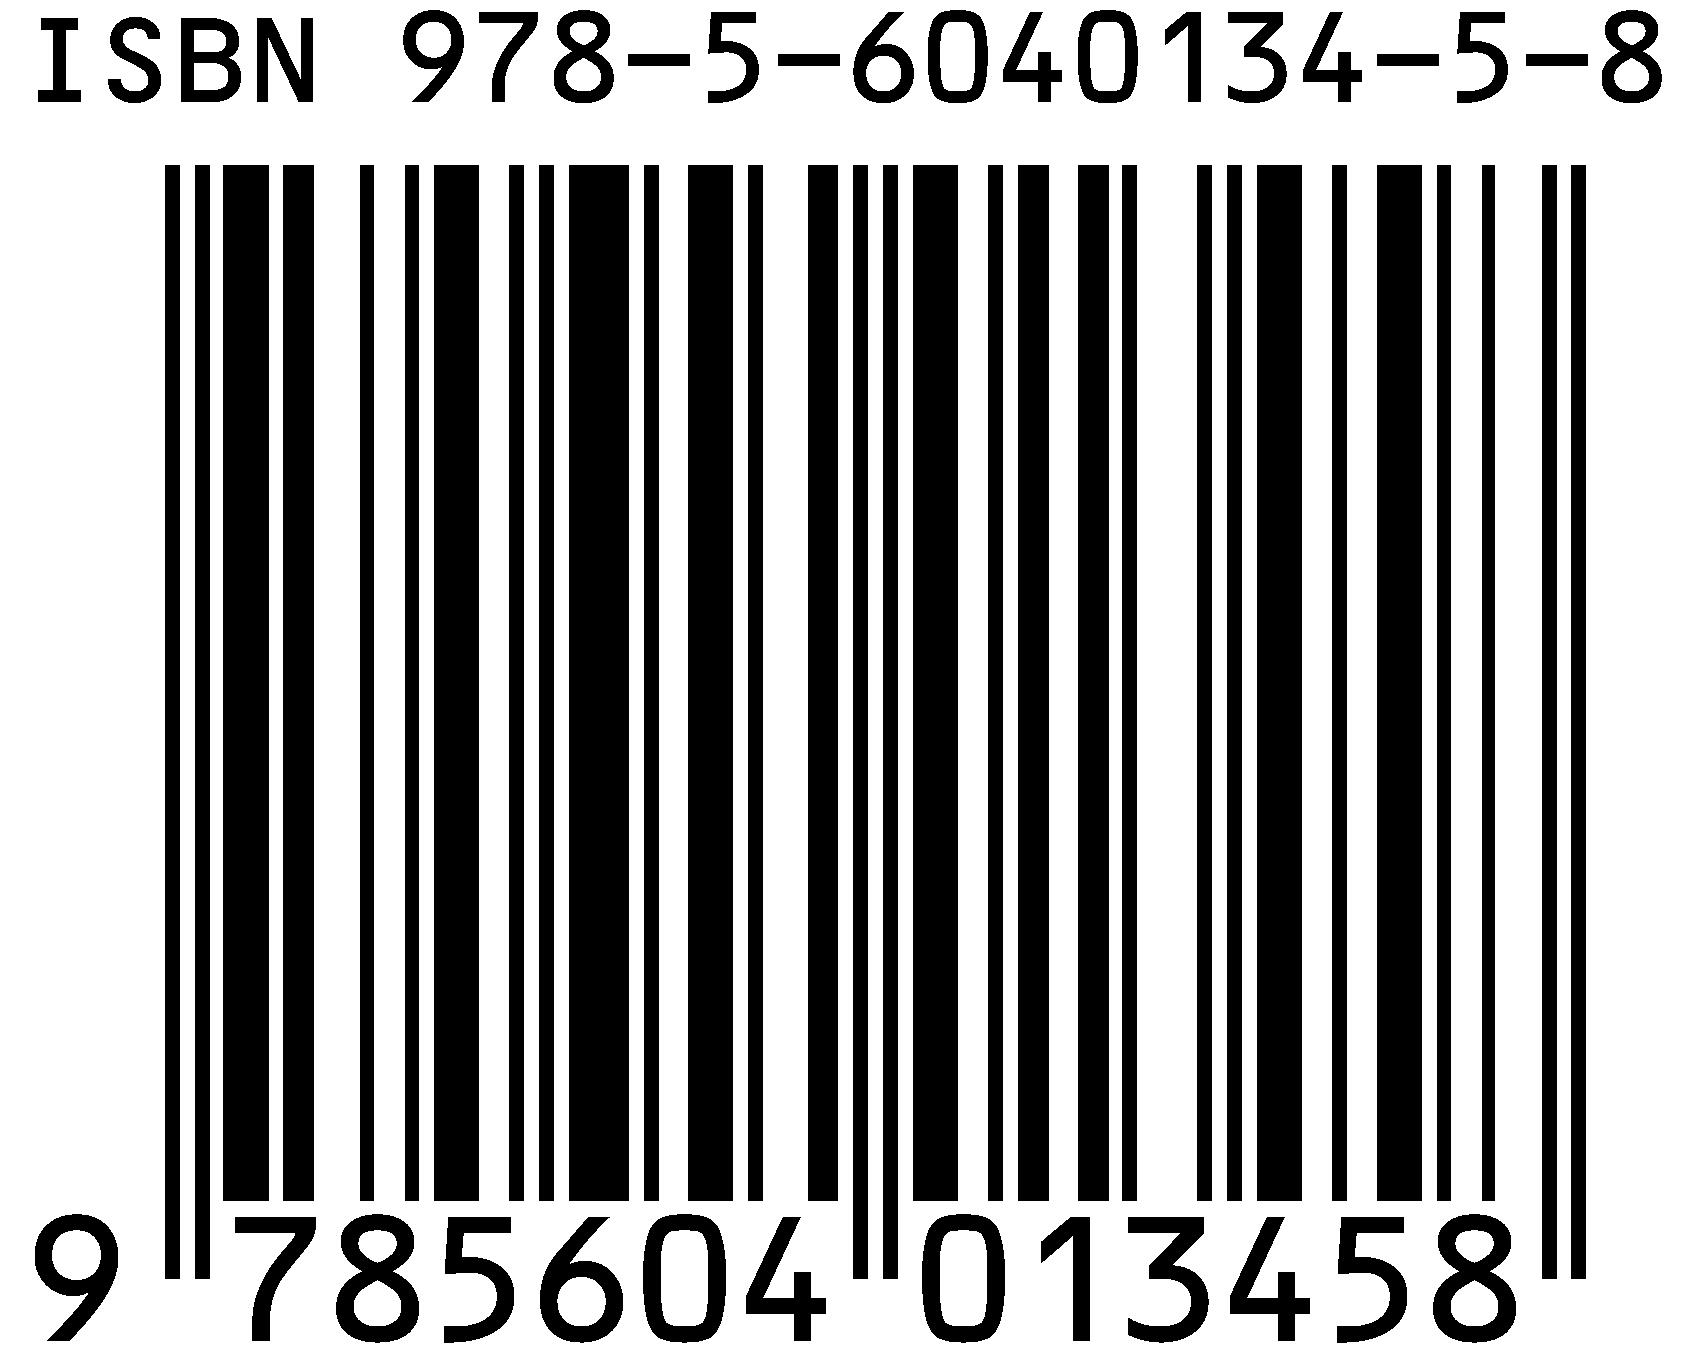
\includegraphics[height=30mm]{ISBN-978-5-6040134-5-8.jpg}
\end{center}


\enlargethispage{5\baselineskip}
\begin{changemargin}{-2cm}{-2cm}
\begin{center}
  \footnotesize
  Подписано в печать ??.??.2020\,г.  Формат 70$\times$108/16. Бумага
  <<Офсетная>>.\hspace*{2em}

  Гарнитура <<Таймс>>. Печать офсетная.  Усл.\,п.\,л. ??.??.
  \rule{1.1\textwidth}{.1mm}\\
  Северо-Восточный комплексный научнo-исследовательский институт им.
  Н.\,А.\,Шило ДВО РАН. \\ 685000, Магадан, ул.\,Портовая, 16.
\end{center}
\end{changemargin}


%%%%%%%%%%%%%%%%%%%%%%%%%%%%%%%%%%%%%%




\end{document}
%%%%%%%%%%%%%%%%%%%%%
%  КОНЕЦ ДОКУМЕНТА  %
%%%%%%%%%%%%%%%%%%%%%
